% This LaTeX document needs to be compiled with XeLaTeX.
\documentclass[10pt]{article}
\usepackage[utf8]{inputenc}
\usepackage{ucharclasses}
\usepackage{amsmath}
\usepackage{amsfonts}
\usepackage{amssymb}
\usepackage[version=4]{mhchem}
\usepackage{extpfeil}
\usepackage{stmaryrd}
\usepackage{graphicx}
\usepackage[export]{adjustbox}
\graphicspath{ {./images/} }
\usepackage{multirow}
\usepackage{bbold}
\usepackage{caption}
\usepackage{hyperref}
\hypersetup{colorlinks=true, linkcolor=blue, filecolor=magenta, urlcolor=cyan,}
\urlstyle{same}
\usepackage[fallback]{xeCJK}
\usepackage{polyglossia}
\usepackage{fontspec}
\IfFontExistsTF{Noto Serif CJK TC}
{\setCJKmainfont{Noto Serif CJK TC}}
{\IfFontExistsTF{STSong}
  {\setCJKmainfont{STSong}}
  {\IfFontExistsTF{Droid Sans Fallback}
    {\setCJKmainfont{Droid Sans Fallback}}
    {\setCJKmainfont{SimSun}}
}}

\setmainlanguage{vietnamese}
\setotherlanguages{english}
\newfontfamily\vietnamesefont{CMU Serif}
\IfFontExistsTF{CMU Serif}
{\newfontfamily\lgcfont{CMU Serif}}
{\IfFontExistsTF{DejaVu Sans}
  {\newfontfamily\lgcfont{DejaVu Sans}}
  {\newfontfamily\lgcfont{Georgia}}
}
\setDefaultTransitions{\lgcfont}{}
\setTransitionsFor{Vietnamese}{\vietnamesefont}{\lgcfont}

\title{Churong 3 \\
 DAICUONG \\
 VEIOA IOC IOU CO }

\author{}
\date{}


\begin{document}
\maketitle
\captionsetup{singlelinecheck=false}
\section*{Phan I div iói va BALTAP}
\section*{Churong 1 CAN BANC IOA IOC}
\section*{BÀI 1}
\section*{KHÁI NIỆM VỀ CÂN BẰNG HOÁ HOC}
\section*{NHAN BUET}
1.1. Phản ứng nào sau đây là phản ứng thuận nghich?\\
A. $\mathrm{Mg}+2 \mathrm{HCl} \longrightarrow \mathrm{MgCl}_{2}+\mathrm{H}_{2}$.\\
B. $2 \mathrm{SO}_{2}+\mathrm{O}_{2} \rightleftharpoons 2 \mathrm{SO}_{3}$.\\
C. $\mathrm{C}_{2} \mathrm{H}_{5} \mathrm{OH}+3 \mathrm{O}_{2} \longrightarrow 2 \mathrm{CO}_{2}+3 \mathrm{H}_{2} \mathrm{O}$.\\
D. $2 \mathrm{KClO}_{3} \longrightarrow 2 \mathrm{KCl}+3 \mathrm{O}_{2}$.\\
1.2. Cho $5 \mathrm{~mol} \mathrm{H}_{2}$ và $5 \mathrm{~mol} \mathrm{I}_{2}$ vào bình kín dung tích 1 lít và nung nóng đến $227^{\circ} \mathrm{C}$ K. Đồ thị biểu diễn sự thay đổi nồng độ các chât theo thời gian được cho trong hinh sau:\\
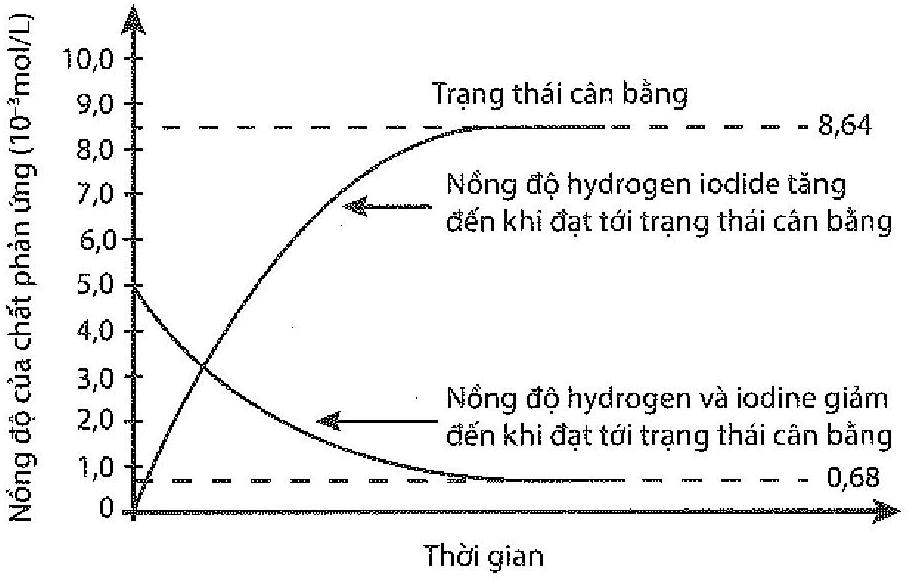
\includegraphics[max width=\textwidth, center]{2025_10_23_fa9073eecee116ad8cf2g-01}

Nồng độ của HI ở trạng thái cân bằng là\\
A. $0,68 \mathrm{M}$.\\
B. $5,00 \mathrm{M}$.\\
C. $3,38 \mathrm{M}$.\\
D. 8,64 M.\\
1.3. Cho phản úng hoá học sau: $\mathrm{Br}_{2}(\mathrm{~g})+\mathrm{H}_{2}(\mathrm{~g}) \rightleftharpoons 2 \mathrm{HBr}(\mathrm{g})$ Biểu thức hằng số cân bằng $\left(K_{C}\right)$ của phản ứng trên là\\
A. $\mathrm{K}_{\mathrm{C}}=\frac{2[\mathrm{HBr}]}{\left[\mathrm{Br}_{2}\right]\left[\mathrm{H}_{2}\right]}$.\\
B. $\mathrm{K}_{\mathrm{C}}=\frac{[\mathrm{HBr}]^{2}}{\left[\mathrm{H}_{2}\right]\left[\mathrm{Br}_{2}\right]}$.\\
C. $\mathrm{K}_{\mathrm{C}}=\frac{\left[\mathrm{H}_{2}\right]\left[\mathrm{Br}_{2}\right]}{[\mathrm{HBr}]^{2}}$.\\
D. $\mathrm{K}_{\mathrm{C}}=\frac{\left[\mathrm{H}_{2}\right]\left[\mathrm{Br}_{2}\right]}{2[\mathrm{HBr}]}$.\\
1.4. Cho phản ứng hoá học sau: $\mathrm{PCl}_{3}(\mathrm{~g})+\mathrm{Cl}_{2}(\mathrm{~g}) \rightleftharpoons \mathrm{PCl}_{5}(\mathrm{~g})$ Ở $\mathrm{T}{ }^{\circ} \mathrm{C}$, nồng độ các chất ở trạng thái cân bằng như sau: $\left[\mathrm{PCl}_{5}\right]=0,059 \mathrm{~mol} /$; $\left[\mathrm{PCl}_{3}\right]=\left[\mathrm{Cl}_{2}\right]=0,035 \mathrm{~mol} / \mathrm{L}$.\\
Hằng số cân bằng $\left(\mathrm{K}_{\mathrm{C}}\right)$ cụa phản úng tại $\mathrm{T}^{\circ} \mathrm{C}$ là\\
A. 1,68 .\\
B. 48,16 .\\
C. 0,02 .\\
D. 16,95 .\\
1.5. Cho phản ứng hoá học sau:\\
$\mathrm{N}_{2}(\mathrm{~g})+3 \mathrm{H}_{2}(\mathrm{~g}) \rightleftharpoons 2 \mathrm{NH}_{3}(\mathrm{~g})$\\
$\Delta_{\mathrm{r}} \mathrm{H}_{298}^{0}=-92 \mathrm{~kJ}$

Yếu tố nào sau đây cần tác động để cân bằng trên chuyển dịch sang phải?\\
A. Thêm chất xúc tác.\\
B. Giảm nồng độ $\mathrm{N}_{2}$ hoặc $\mathrm{H}_{2}$.\\
C. Tăng áp suất.\\
D. Tăng nhiêt độ.\\
1.6. Cân bằng hoá học nào sau đây kuông bị chuyển dịch khi thay đổi áp suât?\\
A. $2 \mathrm{SO}_{2}(\mathrm{~g})+\mathrm{O}_{2}(\mathrm{~g}) \rightleftharpoons 2 \mathrm{SO}_{3}(\mathrm{~g})$\\
B. $\mathrm{C}(\mathrm{s})+\mathrm{H}_{2} \mathrm{O}(\mathrm{g}) \rightleftharpoons \mathrm{CO}(\mathrm{g})+\mathrm{H}_{2}(\mathrm{~g})$\\
C. $\mathrm{PCl}_{3}(\mathrm{~g})+\mathrm{Cl}_{2}(\mathrm{~g}) \rightleftharpoons \mathrm{PCl}_{5}(\mathrm{~g})$\\
D. $3 \mathrm{Fe}(\mathrm{s})+4 \mathrm{H}_{2} \mathrm{O}(\mathrm{g}) \rightleftharpoons \mathrm{Fe}_{3} \mathrm{O}_{4}(\mathrm{~s})+4 \mathrm{H}_{2}(\mathrm{~g})$\\
1.7. Cho cân bằng hoá học sau:\\
$4 \mathrm{NH}_{3}(\mathrm{~g})+5 \mathrm{O}_{2}(\mathrm{~g}) \rightleftharpoons 4 \mathrm{NO}(\mathrm{g})+6 \mathrm{H}_{2} \mathrm{O}(\mathrm{g}) \quad \Delta_{\mathrm{r}} \mathrm{H}_{298}^{0}=-905 \mathrm{~kJ}$.\\
Yếu tố nào sau đây cần tác động để cân bằng trên chuyển dịch sang phải?\\
A. Giảm nhiệt độ.\\
B. Tăng áp suất.\\
C. Giảm nồng độ của $\mathrm{O}_{2}$.\\
D. Thêm xúc tác Pt.

\section*{HONC MILU}
1.8. Cho phản úng hoá học sau: $\mathrm{N}_{2} \mathrm{O}_{4}(\mathrm{~g}) \rightleftharpoons 2 \mathrm{NO}_{2}(\mathrm{~g}) \quad \mathrm{K}_{\mathrm{C}}=4,84 \cdot 10^{-3}$ Phương án nào sau đây là nồng độ của các chất tại thời điểm cân bằng?\\
A. $\left[\mathrm{N}_{2} \mathrm{O}_{4}(\mathrm{~g})\right]=4,84 \cdot 10^{-1} \mathrm{M} ;\left[\mathrm{NO}_{2}(\mathrm{~g})\right]=1,0 \cdot 10^{-4} \mathrm{M}$.\\
B. $\left[\mathrm{N}_{2} \mathrm{O}_{4}(\mathrm{~g})\right]=1,0 \cdot 10^{-1} \mathrm{M} ;\left[\mathrm{NO}_{2}(\mathrm{~g})\right]=4,84 \cdot 10^{-4} \mathrm{M}$.\\
C. $\left[\mathrm{N}_{2} \mathrm{O}_{4}(\mathrm{~g})\right]=1,0 \cdot 10^{-1} \mathrm{M} ;\left[\mathrm{NO}_{2}(\mathrm{~g})\right]=2,20 \cdot 10^{-2} \mathrm{M}$.\\
D. $\left[\mathrm{N}_{2} \mathrm{O}_{4}(\mathrm{~g})\right]=5,0 \cdot 10^{-2} \mathrm{M} ;\left[\mathrm{NO}_{2}(\mathrm{~g})\right]=1,10 \cdot 10^{-2} \mathrm{M}$.\\
1.9. Cho các phản úng hoá học sau:\\
(1) $2 \mathrm{NO}(\mathrm{g})+\mathrm{O}_{2}(\mathrm{~g}) \rightleftharpoons 2 \mathrm{NO}_{2}(\mathrm{~g})$\\
(2) $2 \mathrm{SO}_{2}(\mathrm{~g})+\mathrm{O}_{2}(\mathrm{~g}) \rightleftharpoons 2 \mathrm{SO}_{3}(\mathrm{~g})$\\
(3) $\mathrm{N}_{2}(\mathrm{~g})+3 \mathrm{H}_{2}(\mathrm{~g}) \rightleftharpoons 2 \mathrm{NH}_{3}(\mathrm{~g})$\\
(4) $\mathrm{C}(\mathrm{s})+\mathrm{H}_{2} \mathrm{O}(\mathrm{g}) \rightleftharpoons \mathrm{CO}(\mathrm{g})+\mathrm{H}_{2}(\mathrm{~g})$\\
(5) $\mathrm{CaCO}_{3}(\mathrm{~s}) \rightleftharpoons \mathrm{CaO}(\mathrm{s})+\mathrm{CO}_{2}(\mathrm{~g})$\\
$\Delta_{\mathrm{r}} \mathrm{H}_{298}^{\mathrm{o}}=-115 \mathrm{~kJ}$\\
$\Delta_{\mathrm{r}} \mathrm{H}_{298}^{\circ}=-198 \mathrm{~kJ}$\\
$\Delta_{\mathrm{r}} \mathrm{H}_{298}^{\mathrm{o}}=-92 \mathrm{k}$\\
$\Delta_{\mathrm{r}} \mathrm{H}_{298}^{\circ}=130 \mathrm{~kJ}$\\
$\Delta_{\mathrm{r}} \mathrm{H}_{298}^{\circ}=178 \mathrm{~kJ}$\\
a) Các phản ứng toả nhiệt là\\
A. (1); (2) và (3).\\
B. (1) và (3).\\
C. (1); (2); (4) và (5).\\
D. (1); (2); (3) và (5).\\
b) Khi tăng nhiệt độ, các cân bằng hoá học chuyển dịch theo chiều thuận là\\
A. (1); (2) và (3).\\
B. (1); (2) và (5).\\
C. (4) và (5).\\
D. (3) và (5).\\
c) Khi tăng áp suất, các cân bằng hoá học chuyển dịch theo chiều thuận là\\
A. (1); (2) và (3).\\
B. (1); (3) và (5).\\
C. (2); (3) và (4).\\
D. (3); (4) và (5).\\
1.10. Các kết quả trong bảng sau đây được ghi lại từ hai thí nghiệm giữa khí sulfur dioxide và khí oxygen để tạo thành khí sulfur trioxide ở $600^{\circ} \mathrm{C}$. Tính giá trị $\mathrm{K}_{\mathrm{C}}$ ở hai thí nghiệm và nhận xét kết quả thu được.

\begin{center}
\begin{tabular}{|l|l|l|l|l|l|l|}
\hline
\multirow{2}{*}{} & \multicolumn{3}{|c|}{Nông do các chát o inoi diem ban dau (mol/t)} & \multicolumn{3}{|c|}{Nong do các chát o thoi diem can bang (croll/L)} \\
\hline
 & $8 \mathrm{O}_{2}$ & $\mathrm{O}_{2}$ & $\mathrm{SO}_{3}$ & $\mathrm{SO}_{2}$ & $O_{2}$ & SO, \\
\hline
Thi nobient lis. & 2,000 & 1,500 & 3,000 & 1,500 & 1,250 & 3,500 \\
\hline
Thinghiem 2 & 0,500 & 0 & 0,350 & 0,590 & 0,045 & 0,260 \\
\hline
\end{tabular}
\end{center}

1.11. Polystyrene là một loại nhựa thông dụng được đủng để làm đường ống nước. Nguyên liệu để sản xuất polystyrene là styrene ( $\mathrm{C}_{6} \mathrm{H}_{5} \mathrm{CH}=\mathrm{CH}_{2}$ ). Styrene được điều chế từ phản ứng sau:\\
$\mathrm{C}_{6} \mathrm{H}_{5} \mathrm{CH}_{2} \mathrm{CH}_{3}(\mathrm{~g}) \rightleftharpoons \mathrm{C}_{6} \mathrm{H}_{5} \mathrm{CH}=\mathrm{CH}_{2}(\mathrm{~g})+\mathrm{H}_{2}(\mathrm{~g}) \Delta_{\mathrm{r}} \mathrm{H}_{298}^{\mathrm{o}}=123 \mathrm{~kJ}$\\
Cân bằng hoá học của phản úng trên sẽ chuyển dịch theo chiều nào nếu:\\
a) Tăng áp suât của bình phản ưng.\\
b) Tãng nhiệt độ của phản úng.\\
c) Tăng nồng độ của $\mathrm{C}_{6} \mathrm{H}_{5} \mathrm{CH}_{2} \mathrm{CH}_{3}$.\\
d) Thêm chất xúc tác.\\
e) Tách styrene ra khỏi bình phản úng.\\
1.12, Phosphorus trichloride ( $\mathrm{PCl}_{3}$ ) phản ưng với chlorine ( $\mathrm{Cl}_{2}$ ) tạo thành phosphorus pentachloride ( $\mathrm{PCl}_{5}$ ) theo phán úng:\\
$\mathrm{PCl}_{3}(\mathrm{~g})+\mathrm{Cl}_{2}(\mathrm{~g}) \rightleftharpoons \mathrm{PCl}_{5}(\mathrm{~g})$\\
Cho $0,75 \mathrm{~mol} \mathrm{PCl}_{3}$ và $0,75 \mathrm{~mol} \mathrm{Cl}_{2}$ vào bình kín dung tích 8 lít ở $227^{\circ} \mathrm{C}$. Tính nồng độ các chất ở trạng thái cân bằng, biết giá trị hằng số cân bằng $\mathrm{K}_{\mathrm{C}}$ ở $227^{\circ} \mathrm{C}$ là 49 .

\section*{vANC DUNG}
1.13. Trong một bình kín xảy ra cân bằng hoá học sau:\\
$\mathrm{H}_{2}(\mathrm{~g})+\mathrm{I}_{2}(\mathrm{~g}) \rightleftharpoons 2 \mathrm{HI}(\mathrm{g})$\\
Cho $1 \mathrm{~mol} \mathrm{H}_{2}$ và $1 \mathrm{~mol} \mathrm{I}_{2}$ vào bình kím, dung tích 2 lit. Lượng HI tạo thành theo thời gian được biểu diễn bằng đồ thị sau:\\
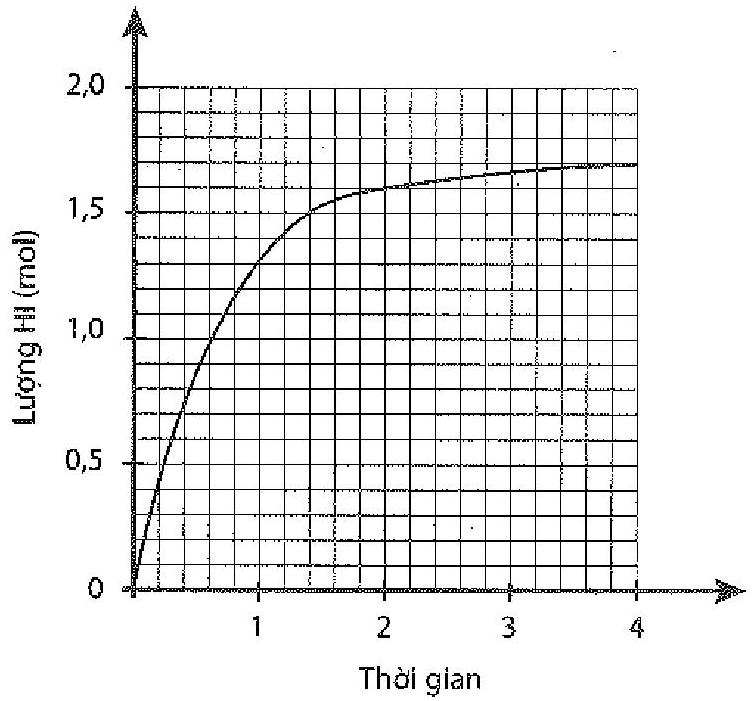
\includegraphics[max width=\textwidth, center]{2025_10_23_fa9073eecee116ad8cf2g-04}\\
a) Xác đinh nồng độ các chất ở thời điểm cân bằng.\\
b) Tính hằng số cân bằng $\mathrm{K}_{\mathrm{C}}$.\\
c) Tính hiệu suất của phån ứng.\\
1.14. Khi xăng cháy trong động co $\hat{O}$ tô sẽ tạo ra nhiệt độ cao, lúc đó $\mathrm{N}_{2}$ phản ứng với $\mathrm{O}_{2}$ tạo thành NO :


\begin{equation*}
\mathrm{N}_{2}(\mathrm{~g})+\mathrm{O}_{2}(\mathrm{~g}) \rightleftharpoons 2 \mathrm{NO}(\mathrm{g}) \tag{1}
\end{equation*}


NO khi đưọc giải phóng ra không khí nhanh chỏng kết họp với $\mathrm{O}_{2}$ tạo thành $\mathrm{NO}_{2}$ là một khí gây ô nhiểm môi trường. Ở $2000^{\circ} \mathrm{C}$, hằng số cân bằng $\mathrm{K}_{\mathrm{c}}$ của phản úng (1) là 0,01.\\
Nếu trong bình kín dung tích 1 lít có $4 \mathrm{~mol} \mathrm{~N}_{2}$ và $0,1 \mathrm{~mol} \mathrm{O}_{2}$ thì ở $2000^{\circ} \mathrm{C}$ lượng khí NO tạo thành là bao nhiêu (giả thiết NO chưa phản úng với $\mathrm{O}_{2}$ )?\\
1.15. Trong dung dịch muối $\mathrm{CoCl}_{2}$ (màu hồng) tồn tại cân bằng hoá học sau:\\
$\left[\mathrm{Co}\left(\mathrm{H}_{2} \mathrm{O}\right)_{6}\right]^{2+}+4 \mathrm{Cl}^{-} \rightleftharpoons\left[\mathrm{CoCl}_{4}\right]^{2-}+6 \mathrm{H}_{2} \mathrm{O} \quad \Delta_{\mathrm{r}} \mathrm{H}_{298}^{\mathrm{o}}>0$ màu hồng màu xanh\\
Dự đoán sự biến đổi màu sắc của ống nghiệm đựng dung dịch $\mathrm{CoCl}_{2}$ trong cảc trương họp sau:\\
a) Thêm từ từ HCl đăc.\\
b) Ngâm ống nghiệm vào cốc nước nóng.\\
c) Thêm một vài giọt dung dịch $\mathrm{AgNO}_{3}$.

\section*{BÀI 2}
\section*{CÂN BẰNG TRONG DUNG DICH NUÚC}
\section*{NHAN BICT}
2.1. Thêm nước vào 10 mL dung dịch $\mathrm{NaOH} 1,0 \mathrm{~mol} / \mathrm{L}$, thu được 1000 mL dung dịch A . Dung dịch A có pH thay đồi như thế nào so với dung dịch ban đầu?\\
A. pH giảm đi 2 đon vị.\\
B. pH giảm đi 1 đơn vị.\\
C. pH tăng 2 đon vi.\\
D. pH tăng gấp đôi.\\
2.2. Trong dung dịch trung hoà về điện, tổng đại số điện tích của cảc ion bằng không. Dung dịch A có chứa $0,01 \mathrm{~mol} \mathrm{Mg}{ }^{2+}, 0,01 \mathrm{~mol} \mathrm{Na}{ }^{+} ; 0,02 \mathrm{~mol} \mathrm{Cl}$ và x mol $\mathrm{SO}_{4}^{2-}$. Giá trị của x là\\
A. 0,01 .\\
B. 0,02 .\\
C. 0,05 .\\
D. 0,005 .\\
2.3. Trong dung dịch nước, cation kim loại mạnh, gốc acid mạnh không bị thuỷ phân, còn cation kim loại trung bình và yếu bị thuỷ phân tạo môi trường acid, gốc acid yếu bị thuỷ phân tạo môi trường base. Dung dịch muối nào sau đây có $\mathrm{pH}>7$ ?\\
A. $\mathrm{KNO}_{3}$.\\
B. $\mathrm{K}_{2} \mathrm{SO}_{4}$.\\
C. $\mathrm{Na}_{2} \mathrm{CO}_{3}$.\\
D. NaCl .\\
2.4. Trong các dung dịch acid sau có cùng nồng đọ $0,1 \mathrm{M}$, dung dịch nào có pH cao nhất?\\
A. HF.\\
B. HCl .\\
C. HBr .\\
D. HI.\\
2.5. Tại khu vực bị ô nhiễm, pH của nước mưa đo được là 4,5 còn pH của nuớc mưa tại khu vực không bị ô nhiễm là 5,7. Nhận xét nào sau đây không đúng?\\
A. Nồng độ ion $\mathrm{H}^{+}$trong dung dịch nước mưa bị ô nhiểm là $10^{-4,5}$.\\
B. Nồng độ ion $\mathrm{H}^{+}$trong dung dịch nước mưa không bị ô nhiểm là $10^{-5,7}$.\\
C. Nồng độ ion $\mathrm{H}^{+}$trong nước mưa bị ô nhiễm thấp hơn so với trong nước mưa không bị ô nhiễm.\\
D. Nồng độ ion OH- trong nước mưa bị ô nhiễm thấp hơn hơn so với trong nước mưa không bị ô nhiễm.

\section*{THONG HIEV}
2.6. Viết phương trình điện li của các chất sau:

\begin{itemize}
  \item Acid yếu: $\mathrm{HCOOH}, \mathrm{HCN}$; acid mạnh: $\mathrm{HCl}, \mathrm{HNO}_{3}$.
  \item Base mạnh: $\mathrm{KOH}, \mathrm{Ba}(\mathrm{OH})_{2}$; base yếu: $\mathrm{Cu}(\mathrm{OH})_{2}$.
  \item Muối: $\mathrm{KNO}_{3}, \mathrm{Na}_{2} \mathrm{CO}_{3}, \mathrm{FeCl}_{3}$.\\
2.7. Dựa vào thuyết acid-base của Brønsted-Lowry, hãy xác định acid, base trong các phản ứng sau:\\
a) $\mathrm{HCOOH}+\mathrm{H}_{2} \mathrm{O} \rightleftharpoons \mathrm{HCOO}^{-}+\mathrm{H}_{3} \mathrm{O}^{+}$\\
b) $\mathrm{HCN}+\mathrm{H}_{2} \mathrm{O} \rightleftharpoons \mathrm{CN}^{-}+\mathrm{H}_{3} \mathrm{O}^{+}$\\
c) $\mathrm{S}^{2-}+\mathrm{H}_{2} \mathrm{O} \rightleftharpoons \mathrm{HS}^{-}+\mathrm{OH}^{-}$\\
d) $\left(\mathrm{CH}_{3}\right)_{2} \mathrm{NH}+\mathrm{H}_{2} \mathrm{O} \rightleftharpoons\left(\mathrm{CH}_{3}\right)_{2} \mathrm{NH}_{2}^{+}+\mathrm{OH}^{-}$\\
2.8. Cho dung dịch HCl 1 M (dung dịch A ) và dung dịch NaOH 1 M (dung dich B ).\\
a) Lấy 10 mL dung dịch A , thêm nước để được 100 mL . Tính pH của dung dịch sau khi pha loãng.\\
b) Lấy 10 mL dung dịch B , thêm nước để được 100 mL . Tính pH của dung dịch sau khi pha loãng.\\
2.9. Một dung dich baking soda $\mathrm{co} \mathrm{pH}=8,3$.\\
a) Môi trường của dung dịch trên là acid, base hay trung tính?\\
b) Tính nồng độ ion $\mathrm{H}^{+}$của dung dịch trên.\\
2.10. Aspirin là một loại thuốc có thành phần chính là acetylsalicylic acid. Nếu hoà tan thuốc này vào nước, người ta xác đinh được pH của dung dịch tạo thành là 2,8. Tính nồng độ $\mathrm{H}^{+}$và nồng $\mathrm{OH}^{-}$của dung dịch tạo thành.
\end{itemize}

\section*{VANTOUNG}
2.11. Hoà tan hoàn toàn a gam CaO vào nước thu được 500 mL dung dịch nước vôi trong (dung dịch A ). Chuẩn độ 5 mL dung dịch A bằng $\mathrm{HCl} 0,1 \mathrm{M}$ thấy hết $12,1 \mathrm{~mL}$.\\
a) Tính nồng độ $\mathrm{Ca}(\mathrm{OH})_{2}$ trong dung dịch nước vôi trong.\\
b) Tính lượng CaO đã bị hoà tan.\\
c) Tính pH của dung dịch nước vôi trong.\\
2.12. Vó trứng có chứa calcium ở dạng $\mathrm{CaCO}_{3}$. Để xác định hàm lượng $\mathrm{CaCO}_{3}$ trong vó trứng, trong phòng thí nghiệm người ta có thể làm như sau:\\
Lấy $1,0 \mathrm{~g}$ vỏ trứng khô, đã được làm sạch, hoà tan hoàn toàn trong 50 mL dung dịch $\mathrm{HCl} 0,4 \mathrm{M}$. Lọc dung dịch sau phản ưng thu được 50 mL dung dịch A . Lấy $10,0 \mathrm{~mL}$ dung dịch A chuẩn độ với dung dịch $\mathrm{NaOH} 0,1 \mathrm{M}$ thấy hết $5,6 \mathrm{~mL}$. Xác định hàm lương calcium trong vỏ trưng (giả thiết các tạp chất khác trong vỏ trứng không phản ứng với HCl ).\\
2.13. Nabica là một loại thuốc có thành phần chính là $\mathrm{NaHCO}_{3}$, được dùng để trung hoà bớt lượng acid HCl dư trong dạ dày.\\
a) Viết phương trình hoá học của phản ứng trung hoà trên.\\
b) Giả thiết nồng dộ düng dịch HCl trong dạ dày là $0,035 \mathrm{M}$, tính thể tích dung dịch HCl được trung hoà khi bệnh nhân uống $0,588 \mathrm{~g}$ bột $\mathrm{NaHCO}_{3}$.\\
2.14. Một học sinh thực hiện thí nghiệm sau: Lấy 10 mL dung dịch $\mathrm{HCl} 0,2 \mathrm{M}$ cho vào 5 mL dung dịch $\mathrm{NH}_{3}$ thu được dung dịch A . Chuẩn độ lượng HCl dư trong dung dịch A bằng dung dịch $\mathrm{NaOH} 0,1 \mathrm{M}$ thấy phản ứng hết $10,2 \mathrm{~mL}$. Tính nồng độ của dung dịch $\mathrm{NH}_{3}$ ban đầu.

\section*{BÀl 3}
\section*{ÔN TÂP CHUONG 1}
\section*{NHAN EILET}
3.1. Cho phản úng hoá học sau:\\
$\mathrm{CH}_{3} \mathrm{COOH}(l)+\mathrm{CH}_{3} \mathrm{OH}(l) \rightleftharpoons \mathrm{CH}_{3} \mathrm{COOCH}_{3}(l)+\mathrm{H}_{2} \mathrm{O}(l)$\\
Biểu thức hằng số cân bằng của phản ứng trên là\\
A. $\mathrm{K}_{\mathrm{C}}=\frac{\left[\mathrm{CH}_{3} \mathrm{COOCH}_{3}\right]\left[\mathrm{H}_{2} \mathrm{O}\right]}{\left[\mathrm{CH}_{3} \mathrm{COOH}\right]\left[\mathrm{CH}_{3} \mathrm{OH}\right]}$,\\
B. $\mathrm{K}_{\mathrm{C}}=\frac{\left[\mathrm{CH}_{3} \mathrm{COOCH}_{3}\right]}{\left[\mathrm{CH}_{3} \mathrm{COOH}\right]\left[\mathrm{CH}_{3} \mathrm{OH}\right]}$.\\
C. $\mathrm{K}_{\mathrm{C}}=\frac{\left[\mathrm{CH}_{3} \mathrm{COOH}\right]\left[\mathrm{CH}_{3} \mathrm{OH}\right]}{\left[\mathrm{CH}_{3} \mathrm{COOCH}_{3}\right]\left[\mathrm{H}_{2} \mathrm{O}\right]}$.\\
D. $\mathrm{K}_{\mathrm{C}}=\frac{\left[\mathrm{CH}_{3} \mathrm{COOH}\right]\left[\mathrm{CH}_{3} \mathrm{OH}\right]}{\left[\mathrm{CH}_{3} \mathrm{COOCH} 3\right]}$.\\
3.2. Cho phản ứng hoá học sau:\\
$3 \mathrm{Fe}(\mathrm{s})+4 \mathrm{H}_{2} \mathrm{O}(\mathrm{g}) \rightleftharpoons \mathrm{Fe}_{3} \mathrm{O}_{4}(\mathrm{~s})+4 \mathrm{H}_{2}(\mathrm{~g})$\\
Biểu thức hằng số cân bằng của phản ứng trên là\\
A. $\mathrm{K}_{\mathrm{C}}=\frac{\left[\mathrm{H}_{2}\right]^{4}\left[\mathrm{Fe}_{3} \mathrm{O}_{4}\right]}{\left[\mathrm{H}_{2} \mathrm{O}\right]^{4}[\mathrm{Fe}]^{3}}$.\\
B. $\mathrm{K}_{\mathrm{C}}=\frac{\left[\mathrm{H}_{2}\right]^{4}}{\left[\mathrm{H}_{2} \mathrm{O}\right]^{4}}$.\\
C. $\mathrm{K}_{\mathrm{C}}=\frac{4\left[\mathrm{H}_{2}\right]}{4\left[\mathrm{H}_{2} \mathrm{O}\right]}$.\\
D. $\mathrm{K}_{\mathrm{C}}=\frac{4\left[\mathrm{H}_{2}\right]\left[\mathrm{Fe}_{3} \mathrm{O}_{4}\right]}{4\left[\mathrm{H}_{2} \mathrm{O}\right] 3[\mathrm{Fe}]}$.\\
3.3. Cho phản ứng hoá học sau:\\
$2 \mathrm{NO}(\mathrm{g})+\mathrm{O}_{2}(\mathrm{~g}) \rightleftharpoons \mathrm{NO}_{2}(\mathrm{~g})$\\
$\Delta_{\mathrm{r}} \mathrm{H}_{298}^{\circ}=-115 \mathrm{~kJ}$

Nhận xét nào sau đây không đúng?\\
A. Nếu tăng nhiệt độ thì cân bằng trên chuyển dịch theo chiều nghịch.\\
B. Nếu tăng áp suất thì cân bằng trên chuyển dịch theo chiều nghịch.\\
C. Hằng số cân bằng của phản ứng trên chỉ phụ thuộc vào nhiệt độ.\\
D. Phản ứng thuận là phản ứng toả nhiệt.\\
3.4. Cho cân bằng hoá học sau: $2 \mathrm{CO}_{2}(\mathrm{~g}) \rightleftharpoons 2 \mathrm{CO}(\mathrm{g})+\mathrm{O}_{2}(\mathrm{~g})$. Ở $\mathrm{T}^{\circ} \mathrm{C}$, nồng độ các chất ở trạng thái cân bằng như sau: $\left[\mathrm{CO}_{2}(\mathrm{~g})\right]=1,2 \mathrm{~mol} / \mathrm{L},[\mathrm{CO}(\mathrm{g})]=0,35 \mathrm{~mol} / \mathrm{L}$ và $\left[\mathrm{O}_{2}(\mathrm{~g})\right]=0,15 \mathrm{~mol} / \mathrm{L}$. Hằng số cân bằng của phản ứng tại $T^{\circ} \mathrm{C}$ là\\
A. $1,276 \cdot 10^{-2}$.\\
B. $4,375 \cdot 10^{-2}$.\\
C. 78,36 .\\
D. 22,85 .\\
3.5. Trong dung dịch nước, cation kim loại mạnh, gốc acid mạnh không bị thuỷ phân, còn cation kim loại trung bình và yếu bị thự phân tạo môi trường acid, gốc acid yếu bị thuỷ phân tạo môi trường base. Dung dịch muối nào sau đây có $\mathrm{pH}<7$ ?\\
A. $\mathrm{FeCl}_{3}$.\\
B. KCl .\\
C. $\mathrm{Na}_{2} \mathrm{CO}_{3}$.\\
D. $\mathrm{Na}_{2} \mathrm{SO}_{4}$.\\
3.6. Trong các dung dịch có cùng nồng độ $0,1 \mathrm{M}$ sau đây, dung dịch nào có pH cao nhất?\\
A. $\mathrm{H}_{2} \mathrm{SO}_{4}$.\\
B. HCl .\\
C. $\mathrm{NH}_{3}$.\\
D. NaOH .

\section*{THONTG HISU}
3.7. Cho phản ứng thuận nghich sau: $\mathrm{H}_{2}(\mathrm{~g})+\mathrm{I}_{2}(\mathrm{~g}) \rightleftharpoons 2 \mathrm{HI}(\mathrm{g})$

Ở $430^{\circ} \mathrm{C}$, nồng độ các chất ở trạng thái cân bằng là: $\left[\mathrm{H}_{2}\right]=\left[\mathrm{I}_{2}\right]=0,107 \mathrm{~mol} / \mathrm{L}$; $[\mathrm{HI}]=0,786 \mathrm{~mol} / \mathrm{L}$.\\
a) Tính hằng số cân bằng ( $\mathrm{K}_{\mathrm{C}}$ ) của phản ứng ở $430^{\circ} \mathrm{C}$.\\
b) Nếu cho $2 \mathrm{~mol} \mathrm{H}_{2}$ và $2 \mathrm{~mol} \mathrm{I}_{2}$ vào bình kín dung tích 10 lít, giữ bình ở $430^{\circ} \mathrm{C}$ thì nồng độ các chất ở trạng thái cân bằng là bao nhiêu?\\
3.8. Methylamine $\left(\mathrm{CH}_{3} \mathrm{NH}_{2}\right)$ là chất có mùi tanh, được sử dụng làm dược phẩm, thuốc trừ sâu,... Trong dung dịch nước methylamin nhận proton của nước. Viết phương trình hoá học của phản ứng giữa methylamine và nước, xác định đâu là acid, base trong phản ứng. Dự đoán môi trường của dung dịch $\mathrm{CH}_{3} \mathrm{NH}_{2}$.\\
3.9. Cho các dung dịch sau: $\mathrm{HCl} 0,1 \mathrm{M} ; \mathrm{H}_{2} \mathrm{SO}_{4} 0,1 \mathrm{M}$ và $\mathrm{CH}_{3} \mathrm{COOH} 0,1 \mathrm{M}$. Sáp xếp các dung dịch trên theo chiều giá trị pH giảm dần. Giải thích.\\
3.10. Dung dịch HCl có $\mathrm{pH}=1$ (dung dịch A ), dung dịch NaOH có $\mathrm{pH}=13$ (dung dịch B). Tính pH của dung dịch sau khi trộn:\\
a) 5 mL dung dịch $A$ và 10 mL dung dich $B$.\\
b) 5 mL dung dich $B$ vào 10 mL dung dịch $A$.\\
c) 10 mL dung dich B vào 10 mL dung dich A .\\
3.11. Ascobic acid (vitamin C) là một acid hữu cơ được kí hięp đơn giản là HAsc, phân tử khối là 176. Mọt học sinh hoà tan $5,0 \mathrm{~g}$ ascorbic acid vào 250 mL nước. Tính pH của dung dịch thu được, biết trong dung dịch có cân bằng sau:\\
$\mathrm{HAsc} \rightleftharpoons \mathrm{H}^{+}+\mathrm{Asc}^{-}$

$$
\mathrm{K}_{\mathrm{a}}=8 \cdot 10^{-5}
$$

\section*{VAN DUNG}
3.12. Ethanol và propanoic acid phån úng với nhau tạo thành ethyl propanoate theo phản úng hoá học sau:

$$
\mathrm{C}_{2} \mathrm{H}_{5} \mathrm{OH}(l)+\mathrm{C}_{2} \mathrm{H}_{5} \mathrm{COOH}(l) \rightleftharpoons \mathrm{C}_{2} \mathrm{H}_{5} \mathrm{COOC} \mathrm{H}_{5}(l)+\mathrm{H}_{2} \mathrm{O}(l)
$$

$\mathrm{O}^{2} 50^{\circ} \mathrm{C}$, giá trị $\mathrm{K}_{\mathrm{C}}$ của phản ứng trên là 7,5 . Nếu cho $23,0 \mathrm{~g}$ ethanol phản úng với $37,0 \mathrm{~g}$ propanoic acid os $50^{\circ} \mathrm{C}$ thì khối lượg của ethyl propanoate thu đưọc trong hỗn hợp ở trạng thái cân bằng là bao nhiêu? (Coi tông thể tích của hệ phản úng không đổi.)\\
3.13. Cho cân bằng hoá học sau:\\
$\mathrm{N}_{2}(\mathrm{~g})+3 \mathrm{H}_{2}(\mathrm{~g}) \rightleftharpoons 2 \mathrm{NH}_{3}(\mathrm{~g})$

$$
\Delta \mathrm{H}=-92 \mathrm{~kJ}
$$

Cho $3,0 \mathrm{~mol}$ khí hydrogen và $1,0 \mathrm{~mol}$ khí nitrogen vào một bình kín dung tích 10 lít, có bột iron xúc tác, giữ bình ở $450{ }^{\circ} \mathrm{C}$. Ở trạng thái cân bằng có $20 \%$ chất đầu chuyền hoá thành sản phẩm.\\
a) Xác định số mol các chất ở trạng thái cân bằng.\\
b) Tính hằng số cân bằng của phản ưng ở nhiệt độ trên.\\
c) Khi tăng nhiệt độ, cân bằng chuyển dịch theo chiều nào?\\
3.14. a) $\mathrm{CH}_{3} \mathrm{COOH}$ (có trong giấm ăn) là một acid yếu. Tính pH của dung dịch $\mathrm{CH}_{3} \mathrm{COOH} 0,1 \mathrm{M}$ (biết hằng số cân bằng của sự phân li $\mathrm{CH}_{3} \mathrm{COOH}$ là $1,8.10^{-5}$, bỏ qua sự phân li của nước).\\
b) Trong dung dịch nước ion $\mathrm{CH}_{3} \mathrm{COO}^{-}$nhận proton của nước. Viết phương trình thuý phân và cho biết môi trường của dung dịch $\mathrm{CH}_{3} \mathrm{COONa}$.\\
c) Cho 10 mL dung dich $\mathrm{NaOH} 0,1 \mathrm{M}$ vào 10 mL dung dịch $\mathrm{CH}_{3} \mathrm{COOH} 0,2 \mathrm{M}$ thu được 20 mL dung dịch A . Tính pH của dung dịch A .\\
3.15. Một học sinh cân $1,062 \mathrm{~g} \mathrm{NaOH}$ rắn rồi pha thành 250 mL dung dịch A .\\
a) Tính nồng độ $\mathrm{C}_{\mathrm{M}}$ của dung dịch A .\\
b) Lấy $5,0 \mathrm{~mL}$ dung dịch A rồi chuẩn độ với dung dịch $\mathrm{HCl} 0,1 \mathrm{M}$ thì thấy hết $5,2 \mathrm{~mL}$. Tính nồng độ dung dịch A từ kết quả chuẩn độ trên.\\
c) Nêu một số nguyên nhân dẫn đến việc sai khác nồng độ dung dịch A trong câu a và b.

\section*{Chuong 2 NITROGEN - SULFUR}
\section*{BÀl 4}
\section*{NITROGEN}
\section*{WHAN BIET}
4.1. Khí nào phổ biến nhất trong khí quyển Trái Đất?\\
A. Oxygen.\\
B. Nitrogen.\\
C. Ozone.\\
D. Argon.\\
4.2. Công thức hoá học của diêm tiêu Chile là\\
A. $\mathrm{Ca}\left(\mathrm{NO}_{3}\right)_{2}$.\\
B. $\mathrm{NH}_{4} \mathrm{NO}_{3}$.\\
C. $\mathrm{NH}_{4} \mathrm{Cl}$.\\
D. $\mathrm{NaNO}_{3}$.\\
4.3. Ví trí (chu kì, nhóm) của nguyên tố nitrogen trong bảng tuần hoàn là\\
A. chu kì 2, nhóm VA.\\
B. chu kì 3, nhóm VA.\\
C. chu kì 2, nhóm VIA.\\
D. chu kì 3, nhóm IVA.\\
4.4. Trong tự nhiên, nguyên tố nitrogen tồn tại trong hợp chất hữu cơ nào sau đây?\\
A. Tinh bột.\\
B. Cellulose.\\
C. Protein.\\
D. Glucose.\\
4.5. Số oxi hoá thấp nhất và cao nhất của nguyên tử nitrogen lần lượt là\\
A. 0 và +5 .\\
B. -3 và 0 .\\
C. -3 và +5 .\\
D. -2 và +4 .\\
4.6. Trong tự nhiên, nguyên tố nitrogen tồn tại chủ yếu ở dạng đồng vị nào sau đầy?\\
A. ${ }^{14} \mathrm{~N}$.\\
B. ${ }^{13} \mathrm{~N}$.\\
C. ${ }^{15} \mathrm{~N}$.\\
D. ${ }^{12} \mathrm{~N}$.\\
4.7. Trong phản ứng tổng hợp ammonia từ nitrogen và hydrogen, nitrogen đóng vai trò là\\
A. chất khử.\\
B. chất oxi hoá.\\
C. acid.\\
D. base.\\
4.8. Trong những con mưa dông kèm sấm sét, nitrogen kết hợp trực tiếp với oxygen tạo thành sản phẩm là\\
A. NO.\\
B. $\mathrm{N}_{2} \mathrm{O}$.\\
C. $\mathrm{NH}_{3}$.\\
D. $\mathrm{NO}_{2}$.\\
4.9. Trong phản úng hoá hợp với oxygen, nitrogen đóng vai trò là\\
A. chất oxi hoá.\\
B. base.\\
C. chất khử.\\
D. acid.\\
4.10. Trong tự nhiên, phản úng giưa nitrogen và oxygen (trong con mưa dông kèm sấm sét) là khởi đầu cho quá trình tạo và cung cấp loại phân bón nào cho cây?\\
A. Phân kali.\\
B. Phân đãm ammonium,\\
C. Phân lân.\\
D. Phân đam nitrate.

\section*{THONG HIGO}
4.11. Áp suất riêng phần của khí nitrogen trong khí quyển là\\
A. 0,21 bar.\\
B. 0,01 bar.\\
C. 0,78 bar.\\
D. 0,28 bar.\\
4.12. Trong tự nhiên, nguyên tố nitrogen có hai đồng vị bền là ${ }^{14} \mathrm{~N}(99,63 \%)$ và ${ }^{15} \mathrm{~N}$ ( $0,37 \%$ ). Nguyên tữ khối trung bình của nitrogen là\\
A. 14,000 .\\
B. 14,004 .\\
C. 14,037 .\\
D. 14,063 .\\
4.13. Số liên kết sigma $(\sigma)$ và số liên kết pi $(\pi)$ trong phân tử nitrogen lần lượt là\\
A. 2 và 1 .\\
B. 0 và 3 .\\
C. 3 và 0 .\\
D. 1 và 2 .\\
4.14. Bậc liên kết và năng lượng liên kết trong phân tữ nitrogen tương ứng là\\
A. 2 và $418 \mathrm{~kJ} / \mathrm{mol}$.\\
B. 1 và $167 \mathrm{~kJ} / \mathrm{mol}$.\\
C. 1 và $386 \mathrm{~kJ} / \mathrm{mol}$.\\
D. 3 và $945 \mathrm{~kJ} / \mathrm{mol}$.\\
4.15. Nitrogen thể hiện tính khử trong phản ứng nào sau đây?\\
A. $\mathrm{N}_{2}+\mathrm{O}_{2} \leftrightharpoons 2 \mathrm{NO}$.\\
B. $\mathrm{N}_{2}+3 \mathrm{H}_{2} \xlongequal[\mathrm{xt}]{\mathrm{t}^{\mathrm{o}}, \mathrm{p}} 2 \mathrm{NH}_{3}$.\\
C. $3 \mathrm{Ca}+\mathrm{N}_{2} \xrightarrow{t^{\circ}} \mathrm{Ca}_{3} \mathrm{~N}_{2}$.\\
D. $3 \mathrm{Mg}+\mathrm{N}_{2} \xrightarrow{\mathrm{t}^{\mathrm{a}}} \mathrm{Mg}_{3} \mathrm{~N}_{2}$.\\
4.16. Nhận định nào sau đây về phân tử nitrogen là đúng?\\
A. Có ba liên kết đơn bền vững.\\
B. Chứa nguyên tử nitrogen có số oxi hoá là -3 .\\
C. Có liên kết công hoá trị có cưc.\\
D. Thể hiện cả tính oxi hoá và tính khử.\\
4.17. Nhận định nào sau đây về đơn chất nitrogen là sai?\\
A. Không màu và nhẹ hơn không khí.\\
B. Hoá hợp với oxygen ở nhiệt độ cao hoặc tia lửa điện.\\
C. Thể hiện tính oxi hoá mạnh ở điều kiện thường.\\
D. Khó hoá lỏng và ít tan trong nước.\\
4.18. Trong nghiên cứu, khí nitrogen thường được dùng để tạo bầu khí quyển trơ dựa trên cơ sở nào?\\
A. Nitrogen có tính oxi hoá mạnh.\\
B. Nitrogen rất bền với nhiệt.\\
C. Nitrogen khó hoá lỏng.\\
D. Nitrogen không có cực.\\
4.19. Cho sơ đồ chuyển hoá nitrogen trong khí quyển thành phân đạm:

$$
\mathrm{N}_{2} \xrightarrow{+\mathrm{O}_{2}} \mathrm{NO} \xrightarrow{+\mathrm{O}_{2}} \mathrm{NO}_{2} \xrightarrow{+\mathrm{O}_{2}+\mathrm{H}_{2} \mathrm{O}} \mathrm{HNO}_{3} \longrightarrow \mathrm{NO}_{3}^{-}
$$

Số phản ứng thuộc loại oxi hoá-khử trong sơ đồ là\\
A. 3 .\\
B. 1 .\\
C. 4 .\\
D. 2 .\\
4.20. Tính phân tử khối trung bình của không khí, giả thiết thành phần không khí: 78\% nitrogen, 21\% oxygen và 1\% argon.

\section*{VAN DUNG}
4.21. Tính khối lượng riêng ( $g / L$ ) của không khí ở điều kiện chuẩn, giả thiết thành phần không khí: 78\% nitrogen, 21\% oxygen và 1\% argon.\\
4.22. Trong công nghiệp, ammonia được sản xuất theo phản ứng pha khí:\\
$\mathrm{N}_{2}(\mathrm{~g})+3 \mathrm{H}_{2}(\mathrm{~g}) \longrightarrow 2 \mathrm{NH}_{3}(\mathrm{~g}) \quad \Delta_{\mathrm{r}} \mathrm{H}^{\circ}$\\
Cho biết các giá trị năng lượng liên kết $\mathrm{E}_{\mathrm{b}}\left(\mathrm{kJ} \cdot \mathrm{mol}^{-1}\right)$ :

\begin{center}
\begin{tabular}{|c|c|c|c|}
\hline
Lien ket and & $\mathrm{N} \equiv \mathrm{N}$ & $\mathrm{H}-\mathrm{H}$ & $\mathrm{N}-\mathrm{H}$ \\
\hline
\end{tabular}
\end{center}

a) Tính nhiệt phản ứng $\Delta_{\mathrm{r}} \mathrm{H}^{\circ}$ của phản ứng ở điều kiện chuẩn, nhận xét về dấu và độ lớn của giá trị tìm được.\\
b) Tính nhiệt tạo thành $\Delta_{\mathrm{f}} \mathrm{H}^{\circ}\left(\mathrm{kJ} \cdot \mathrm{mol}^{-1}\right)$ của $\mathrm{NH}_{3}(\mathrm{k})$.\\
4.23. Hỗn hợp X gồm $\mathrm{N}_{2}$ và $\mathrm{H}_{2}$ có ti lệ mol tưong úng là 1: 3. Nung nóng X trong bình kín ( $450^{\circ} \mathrm{C}$, xúc tác Fe) một thời gian, thu được hồn hợ khí có số mol giảm $5 \%$ so với ban đầu. Tính hię̂u suất của phản ưng tồng họp $\mathrm{NH}_{3}$.\\
4.24. Cho cân bằng ở $1650^{\circ} \mathrm{C}: \mathrm{N}_{2}(\mathrm{~g})+\mathrm{O}_{2}(\mathrm{~g}) \rightleftharpoons 2 \mathrm{NO}(\mathrm{g}) \quad \mathrm{K}_{\mathrm{C}}=4 \cdot 10^{-4}$

Thực hiện phản ứng trên vởi một hỗn hợp nitrogen và oxygen có tỉ lệ mol tương ứng là $4: 1$. Tính hiệu suất của phản ưng khi hệ cân bằng ở $1650^{\circ} \mathrm{C}$.\\
4.25. Sau mỗi chu trình tổng họp ammonia đều thực hiện tách ammonia khỏi hỗn họp khí gồm: nitrogen, hydrogen và ammonia. Sau đó, nitrogen và hydrogen lại được dẫn về thực hiện vòng tuần hoàn mới.\\
Cho biết nhiệt độ sôi nitrogen, hydrogen và ammonia lần lượt 1 à $-196^{\circ} \mathrm{C}$, $-253^{\circ} \mathrm{C}$ và $-33^{\circ} \mathrm{C}$.\\
Đề xuất phương pháp vật lí tách ammonia khỏi hỗn họp đó.

\section*{BÀI 5}
\section*{AMMONIA • MUÓI AMMONIUM}
\section*{NHAN TILM}
5.1. Ở trạng thái lỏng nguyên chất, phân tữ chất nào sau đây tạo được liên kết hydrogen với nhau?\\
A. Nitrogen.\\
B. Ammonia.\\
C. Oxygen.\\
D. Hydrogen.\\
5.2. Khí nào sau đây dễ tan trong nước do tạo được liên kết hydrogen với nước?\\
A. Nitrogen.\\
B. Hydrogen.\\
C. Ammonia.\\
D. Oxygen.\\
5.3. Nhận định nào sau đây vè phân tử ammonia không đúng?\\
A. Phân cực mạnh.\\
B. Có một cặp electron không liên kết.\\
C. Có độ bền nhiệt rất cao.\\
D. Có khả năng nhận proton.\\
5.4. Khi tác dụng với nước và hydrochloric acid, ammonia đóng vai trò là\\
A. acid.\\
B base.\\
C. chất oxi hoá.\\
D. chất khư.\\
5.5. Trong phưong pháp Ostwald, ammonia bị oxi hoá bởi oxygen không khí tạo thành sản phấm chinh là\\
A. NO.\\
B. $\mathrm{N}_{2}$.\\
C. $\mathrm{N}_{2} \mathrm{O}$.\\
D. $\mathrm{NO}_{2}$,\\
5.6. Cho dung dịch $\mathrm{NH}_{3}$ vào dung dịch chất nào sau đây thu được kết tủa trắng?\\
A. HCl .\\
B. $\mathrm{H}_{2} \mathrm{SO}_{4}$.\\
C. $\mathrm{H}_{3} \mathrm{PO}_{4}$.\\
D. $\mathrm{AlCl}_{3}$.\\
5.7. Cho vài giọt dung dịch phenolphthalein vào dung dịch $\mathrm{NH}_{3}$, phenolphthalein chuyền sang màu nào sau đây?\\
A. Hồng.\\
B. Xanh.\\
C. Không màu.\\
D. Vàng.\\
5.8. Nhiệt phân hoàn toàn muối nào sau đây thu được sản phẩm chỉ gồm khí và hơi?\\
A. NaCl .\\
B. $\mathrm{CaCO}_{3}$.\\
C. $\mathrm{KClO}_{3}$,\\
D. $\left(\mathrm{NH}_{4}\right)_{2} \mathrm{CO}_{3}$.\\
5.9. Phân biệt được dung dịch $\mathrm{NH}_{4} \mathrm{Cl}$ và NaCl bằng thuốc thử là dung dịch\\
A. KCl .\\
B. $\mathrm{KNO}_{3}$.\\
C. KOH.\\
D. $\mathrm{K}_{2} \mathrm{SO}_{4}$.\\
5.10. Trong nước, phân tư/ion nào sau đây thể hiện vai trò là acid Bronsted?\\
A. $\mathrm{NH}_{3}$.\\
B. $\mathrm{NH}_{4}^{+}$.\\
C. $\mathrm{NO}_{3}^{-}$.\\
D. $\mathbb{N}_{2}$.

\section*{THONC HEU}
5.11. Cho các nhận định sau: Phân tứ ammonia và ion ammonium đều\\
(1) chưa liên kết cộng hoá trị; (2) là base Bronsted trong nước; (3) là acid Brønsted trong nước; (4) chứa nguyên tử N có số oxi hoá là -3.\\
Số nhận định đúng là\\
A. 2 .\\
B. 1 .\\
C. 4 .\\
D. 3 .\\
5.12. Các chất khí được thu vào bình theo đúng nguyên tắc bằng cách đẩy không khí $(\mathrm{X}, \mathrm{Y}, \mathrm{Z})$ và đẩy nước (T) như sau:\\
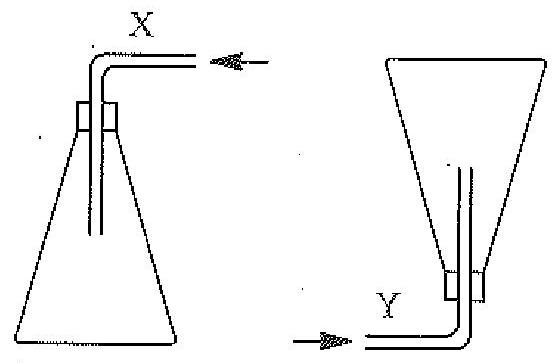
\includegraphics[max width=\textwidth, center]{2025_10_23_fa9073eecee116ad8cf2g-15(1)}\\
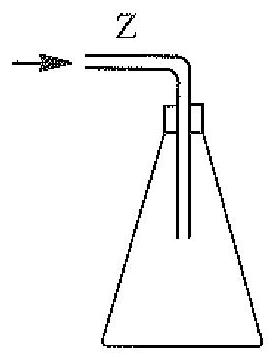
\includegraphics[max width=\textwidth, center]{2025_10_23_fa9073eecee116ad8cf2g-15}\\
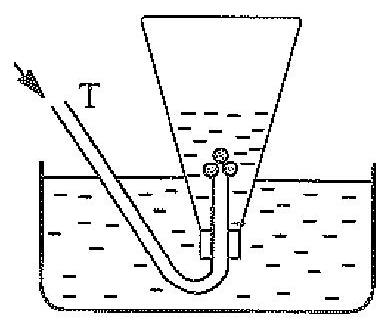
\includegraphics[max width=\textwidth, center]{2025_10_23_fa9073eecee116ad8cf2g-15(2)}

Nhận xét nào sau đây không đúng?\\
A. X là chlorine.\\
B. Y là hydrogen.\\
C. Z là nitrogen dioxide.\\
D. T là ammonia.\\
5.13. Phát biểu nào sau đây không đúng?\\
A. Ammonia là base Brønsted khi tác dụng với nước.\\
B. Ammonia được sữ dụng là chất làm lạnh.\\
C. Muối ammonium là tinh thể ion, dễ tan trong nước.\\
D. Các muối ammonium đều rất bền với nhiêt.\\
5.14. Tiến hành thí nghiệm trộn từng cặp dung dịch sau: (a) $\mathrm{NH}_{3}$ và $\mathrm{AlCl}_{3}$; (b) $\left(\mathrm{NH}_{4}\right)_{2} \mathrm{SO}_{4}$ và $\mathrm{Ba}(\mathrm{OH})_{2}$; (c) $\mathrm{NH}_{4} \mathrm{Cl}$ và $\mathrm{AgNO}_{3}$; (d) $\mathrm{NH}_{3}$ và HCl .

Sau khi phản ứng kết thúc, số thí nghiệm thu được kết tủa là\\
A. 1 .\\
B. 3 .\\
C. 2 .\\
D. 4 .\\
5.15. Xét cân bằng hoá học: $\mathrm{NH}_{3}+\mathrm{H}_{2} \mathrm{O} \rightleftharpoons \mathrm{NH}_{4}^{+}+\mathrm{OH}^{-}$.

Cân bằng sẽ chuyển dịch theo chiều thuận khi cho thêm vài giọt dung dịch nào sau đây?\\
A. $\mathrm{NH}_{4} \mathrm{Cl}$.\\
B. NaOH .\\
C. HCl .\\
D. NaCl .\\
5.16. Xét cân bằng hoá học:\\
$\mathrm{NH}_{3}+\mathrm{H}_{2} \mathrm{O} \rightleftharpoons \mathrm{NH}_{4}^{+}+\mathrm{OH}^{-}$\\
Hằng số cân bằng ( $\mathrm{K}_{\mathrm{C}}$ ) của phản ứng được biểu diễn bằng biểu thúc nào sau đây?\\
A. $\mathrm{K}_{\mathrm{C}}=\frac{\left[\mathrm{NH}_{4}^{+}\right]\left[\mathrm{OH}^{-}\right]}{\left[\mathrm{NH}_{3}\right]}$.\\
B. $\mathrm{K}_{\mathrm{C}}=\frac{\left[\mathrm{NH}_{4}^{+}\right]\left[\mathrm{OH}^{-}\right]}{\left[\mathrm{NH}_{3}\right]\left[\mathrm{H}_{2} \mathrm{O}\right]}$.\\
C. $\mathrm{K}_{\mathrm{C}}=\frac{\left[\mathrm{NH}_{4}^{+}\right]\left[\mathrm{OH}^{-}\right]}{\left[\mathrm{H}_{2} \mathrm{O}\right]}$.\\
D. $\mathrm{K}_{\mathrm{C}}=\frac{\left[\mathrm{NH}_{4}^{+}\right]}{\left[\mathrm{NH}_{3}\right]}$.\\
5.17. Xét cân bằng hoá học: $\mathrm{N}_{2}(\mathrm{k})+3 \mathrm{H}_{2}(\mathrm{k}) \rightleftharpoons 2 \mathrm{NH}_{3}(\mathrm{k}) \quad \Delta \mathrm{H}<0$. Hiệu suất phản ứng khi hệ đạt cân bằng ơ nhiệt độ $400^{\circ} \mathrm{C}$ và $500^{\circ} \mathrm{C}$ lần lượt bằng $\mathrm{x} \%$ và $\mathrm{y} \%$. Mối quan hệ giữa x và y là\\
A. $x<y$.\\
B. $x=y$.\\
C. $x>y$.\\
D. $5 x=4 y$.\\
5.18. Xét cân bằng hoá học: $\mathrm{N}_{2}(\mathrm{~g})+3 \mathrm{H}_{2}(\mathrm{~g}) \rightleftharpoons 2 \mathrm{NH}_{3}(\mathrm{~g}) \quad \Delta \mathrm{H}<0$. Hiệu suất phản ứng khi hệ đạt cân bằng ở áp suất 200 bar và 300 bar lần lượt bằng $\mathrm{x} \%$ và $\mathrm{y} \%$. Mối quan hệ giữa x và y là\\
A. $5 x=4 y$.\\
B. $x=y$.\\
C. $x>y$.\\
D. $x<y$.\\
5.19. Hỗn hợp X gồm $\mathrm{N}_{2}$ và $\mathrm{H}_{2}$ có tỉ lệ mol tương úng là 1 : 4. Nung nóng X trong bình kín ở nhiệt độ khoảng $450^{\circ} \mathrm{C}$ có bột Fe xúc tác, thu được hỗn hợp khí Y có tỉ khối so với $\mathrm{H}_{2}$ bằng 4 . Hiệu suất của phản ứng tồng họp $\mathrm{NH}_{3}$ là\\
A. $20 \%$.\\
B. $25 \%$.\\
C. $30 \%$.\\
D. $10 \%$.\\
5.20. Hỗn hợ khí X gồm $\mathrm{N}_{2}$ và $\mathrm{H}_{2}$ có tí khối đối với $\mathrm{H}_{2}$ bằng 3,6. Nung nóng X trong bình kín có bột Fe xúc tác, thu được hỗn họp khí Y có số mol giảm 8\% so với ban đầu. Hiệu suât của phản úng tổng họp $\mathrm{NH}_{3}$ là\\
A. $25 \%$.\\
B. $23 \%$.\\
C. $16 \%$.\\
D. $20 \%$.

\section*{VAN DUNG}
5.21. a) Viết phương trình hoá học xảy ra khi cho dung dịch $\left(\mathrm{NH}_{4}\right)_{2} \mathrm{CO}_{3}$ lần lượt tác dưng với lượng dư các dung dịch: $\mathrm{HCl}, \mathrm{Ba}(\mathrm{OH})_{2}$.\\
b) Trình bày phương pháp hoá học phân biệt ba dung dịch: $\mathrm{NH}_{4} \mathrm{NO}_{3}, \mathrm{KNO}_{3}, \mathrm{NH}_{4} \mathrm{Cl}$.\\
5.22. Sự phụ thuộc của độ tan khí ammonia trong nước vào nhiệt độ được mô tả ở hinh bên.

Dựa vào đồ thị ở hình bên, hãy xác định:\\
a) Độ tan của ammonia ở $30^{\circ} \mathrm{C}$. Nhận xét về tính tan của ammonia ở nhiệt độ này.\\
b) Nồng độ phần trăm của dung dịch ammonia bão hoà ở $30^{\circ} \mathrm{C}$.\\
c) Dộ tan của ammonia ở $60^{\circ} \mathrm{C}$. So sánh với độ tan của ammonia ở $30^{\circ} \mathrm{C}$. Giải thích.\\
5.23. Trong công nghiệp, nitrogen đượ sản

\begin{figure}[h]
\begin{center}
  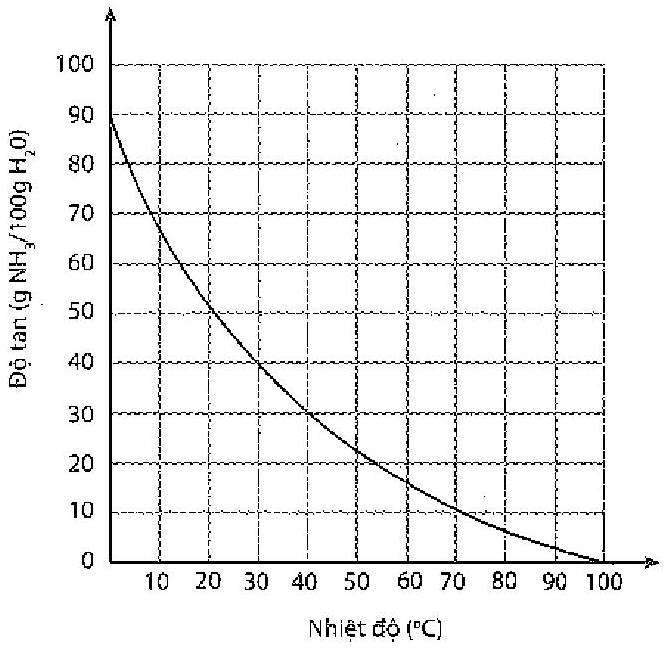
\includegraphics[width=\textwidth]{2025_10_23_fa9073eecee116ad8cf2g-17}
\captionsetup{labelformat=empty}
\caption{Sư phu thuộc của độ tan khí ammonia vào nhiệt độ}
\end{center}
\end{figure}

Cho biết nhiệt độ sôi của các chất trên lần lượt là $-196^{\circ} \mathrm{C},-183^{\circ} \mathrm{C}$ và $-186^{\circ} \mathrm{C}$. Em hãy nêu nguyên tắc sản xuất $\mathrm{N}_{2}$ từ không khí.\\
5.24. Xét cân bằng của dung dịch $\mathrm{NH}_{3} 0,1 \mathrm{M}$ ờ $25^{\circ} \mathrm{C}$ :

$$
\mathrm{NH}_{3}+\mathrm{H}_{2} \mathrm{O} \rightleftharpoons \mathrm{NH}_{4}^{+}+\mathrm{OH}^{-} \quad \mathrm{K}_{\mathrm{C}}=1,74 \cdot 10^{-5}
$$

Bỏ qua sự phân li của nước. Xác định giá trị pH của dung dịch trên.\\
5.25. Xét cân bằng trong dung dịch gồm $\mathrm{NH}_{4} \mathrm{Cl} 0,10 \mathrm{M}$ và $\mathrm{NH}_{3} 0,05 \mathrm{M}$ ở $25^{\circ} \mathrm{C}$ :

$$
\mathrm{NH}_{3}+\mathrm{H}_{2} \mathrm{O} \rightleftharpoons \mathrm{NH}_{4}^{+}+\mathrm{OH}^{-} \quad \mathrm{K}_{\mathrm{C}}=1,74 \cdot 10^{-5}
$$

Bỏ qua sự phân li của nước. Xác định giá trị pH của dung dịch trên.\\
5.26. Tại một nhà máy phân bón, ammophos được sản xuất từ ammonia và phosphoric acid, thu được $\mathrm{NH}_{4} \mathrm{H}_{2} \mathrm{PO}_{4}$ và $\left(\mathrm{NH}_{4}\right)_{2} \mathrm{HPO}_{4}$ vói tí lệ mol là $1: 1$.\\
a) Viết các phưong trình hoá học.\\
b) Tính thể tich khí ammonia (đlce) cần dùng để tác dụng vita đủ với dung dịch chứa 5,88 tấn phosphoric acid. Tính khối lượng ammophos thu được.

\section*{BÀl 6}
\section*{MỘT SỐ HỢ CHÁT VÓI OXYGEN CỦA NITROGEN}
\section*{NHAN BICT}
\begin{enumerate}
  \setcounter{enumi}{5}
  \item 
  \begin{enumerate}
    \item Oxide của nitrogen được tạo thành ở nhiệt độ rất cao, khi nitrogen có trong không khí bị oxi hoá được gọi là\\
A. $\mathrm{NO}_{\mathrm{x}}$ tức thời.\\
B. $\mathrm{NO}_{\mathrm{x}}$ nhiệt.\\
C. $\mathrm{NO}_{\mathrm{x}}$ nhiên liệu.\\
D. $\mathrm{NO}_{\mathrm{x}}$ tự nhiên.\\
6.2. Oxide của nitrogen được tạo thành khi nguyên tố nitrogen trong nhiên liệu hoặc sinh khối kết hợp với oxygen dư thừa trong không khí được gọi là\\
A. NOx nhiên liệu.\\
B. NO, tự nhiên.\\
C. $\mathrm{NO}_{\mathrm{x}}$ tức thời.\\
D. $\mathrm{NO}_{\mathrm{x}}$ nhiêt.\\
6.3. Oxide của nitrogen được tạo thành khi nitrogen trong không khí tác dụng với các gốc tụ do được gọi là\\
A. $\mathrm{NO}_{\mathrm{x}}$ nhiệt.\\
B. $\mathrm{NO}_{\mathrm{x}}$ tức thời.\\
C. $\mathrm{NO}_{\mathrm{x}}$ tư nhiên.\\
D. NO, nhiên liệu.\\
6.4. Nitrogen monoxide được tạo thành khi mưa dông kèm theo sấm sét do phản úng giữa nitrogen và oxygen trong không khí được goi là\\
A. $\mathrm{NO}_{\mathrm{x}}$ nhiên liệu.\\
B. $\mathrm{NO}_{\mathrm{x}}$ túc thời.\\
C. $\mathrm{NO}_{\mathrm{x}}$ tự nhiên.\\
D. NO, nhiệt.\\
6.5. Mưa acid là hiện tượng nước mưa có pH thấp hơn 5,6 (giá trị pH của khí carbon dioxide bão hoà trong nước). Hai tác nhân chính gây mưa acid là\\
A. $\mathrm{Cl}_{2}, \mathrm{HCl}$.\\
B. $\mathrm{N}_{2}, \mathrm{NH}_{3}$.\\
C. $\mathrm{SO}_{2}, \mathrm{NO}_{\mathrm{x}}$.\\
D. $\mathrm{S}, \mathrm{H}_{2} \mathrm{~S}$.\\
6.6. Số oxi hoá thấp nhất của nitrogen là\\
A. -3 .\\
B. 0.\\
C. +1 .\\
D. +4 .\\
6.7. Phân tử nào sau đây có chưa một liên kết cho - nhận?\\
A. $\mathrm{NH}_{3}$.\\
B. $\mathrm{N}_{2}$.\\
C. $\mathrm{HNO}_{3}$.\\
D. $\mathrm{H}_{2}$.\\
6.8. Acid nào sau đây thể hiện tính oxi hoá mạnh khi tác dụng với chất khử?\\
A. HCl .\\
B. $\mathrm{HNO}_{3}$.\\
C. HBr.\\
D. $\mathrm{H}_{3} \mathrm{PO}_{4}$.\\
6.9. Kim loại nào sau đây không tác dụng với nitric acid?\\
A. $\mathbb{Z n}$.\\
B. Cu .\\
\href{http://C.Ag}{C.Ag}.\\
D. Au.\\
6.10. Hiện tượng phú dương là một biểu hiệu của môi trường ao, hồ bị ồ nhiễm do dư thừa các chất dinh dưỡng. Sự đư thừa dinh dưỡng chủ yếu do hàm lượng các ion nào sau đây vượt quá mức cho phép?\\
A. Sodium, potassium.\\
B. Calcium, magnesium.\\
C. Nitrate, phosphate.\\
D. Chloride, sulfate.
  \end{enumerate}
\end{enumerate}

\section*{THONGHILU}
6.11. Cho các nhận định sau về tính chất hoá học của nitric acid: (1) có tính acid mạnh; (2) có tính acid yếu; (3) có tính oxi hoá mạnh; (4) có tính khử mạnh. Số nhận định đúng là\\
A. 1 .\\
B. 2 .\\
C. 3 .\\
D. 4 .\\
6.12. Phát biểu nào sau đây không đúng?\\
A. $\mathrm{NH}_{3}$ và HCl đều dễ tan trong nước.\\
B. $\mathrm{HNO}_{3}$ và HCl đều là acid mạnh trong nước.\\
C. $\mathrm{N}_{2}$ và $\mathrm{Cl}_{2}$ đều có tính oxi hoá mạnh ở điều kiện thường.\\
D. $\mathrm{KNO}_{3}$ và $\mathrm{KClO}_{3}$ đều bị phân huỷ bởi nhiệt.\\
6.13. Phát biểu nào sau đây đúng?\\
A. $\mathrm{N}_{2}$ và P đều tác dụng với oxygen ở nhiệt độ cao.\\
B. $\mathrm{N}_{2}$ và P đều là chất khí ở điều kiện thường.\\
C. $\mathrm{HNO}_{3}$ và $\mathrm{H}_{3} \mathrm{PO}_{4}$ đều có tính oxi hoá mạnh.\\
D. $\mathrm{HNO}_{3}$ và $\mathrm{H}_{3} \mathrm{PO}_{4}$ đểu là acid mạnh.\\
6.14. Xét phản úng trong quá trình tạo ra $\mathrm{NO}_{\mathrm{x}}$ rhiệt:\\
$\mathrm{N}_{2}(\mathrm{~g})+\mathrm{O}_{2}(\mathrm{~g}) \longrightarrow 2 \mathrm{NO}(\mathrm{g}) \quad \Delta_{\mathrm{r}} \mathrm{H}_{298}^{0}=180,6 \mathrm{~kJ}$\\
Nhiệt tạo thành chuẩn của $\mathrm{NO}(\mathrm{g})$ là\\
A. $180,6 \mathrm{~kJ} / \mathrm{mol}$.\\
B. $-180,6 \mathrm{~kJ} / \mathrm{mol}$.\\
C. $-90,3 \mathrm{~kJ} / \mathrm{mol}$.\\
D. $90,3 \mathrm{~kJ} / \mathrm{mol}$.\\
6.15. Xét cân bằng tạo ra nitrogen(H) oxide ở nhiệt độ $2000^{\circ} \mathrm{C}$ :\\
$\mathrm{N}_{2}(\mathrm{~g})+\mathrm{O}_{2}(\mathrm{~g}) \rightleftharpoons 2 \mathrm{NO}(\mathrm{g})$\\
$\mathrm{K}_{\mathrm{C}}=4,10 \cdot 10^{-4}$\\
Ờ trạng thái cân bằng, biểu thức nào sau đây có giá trị bằng $\mathrm{K}_{\mathrm{C}}$ ?\\
A. $\frac{[\mathrm{NO}]^{2}}{\left[\mathrm{~N}_{2}\right]\left[\mathrm{O}_{2}\right]}$.\\
B. $\frac{[\mathrm{NO}]}{\left[\mathrm{N}_{2}\right]\left[\mathrm{O}_{2}\right]}$.\\
C. $\frac{\left[\mathrm{N}_{2}\right]\left[\mathrm{O}_{2}\right]}{[\mathrm{NO}]^{2}}$.\\
D. $\frac{[\mathrm{NO}]}{\left[\mathrm{N}_{2}\right]}$.\\
6.16. Cho các nhận định sau về cấu tạo phân tử nitric acid:\\
(a) Liên kết $\mathrm{O}-\mathrm{H}$ phân cực về oxygen.\\
(b) Nguyên tữ N có số oxi hoá là +5 .\\
(c) Nguyên tử N có hoá tri bằng 4.\\
(d) Liên kết cho - nhận $\mathrm{N} \rightarrow \mathrm{O}$ kém bền.

Số nhận định đúng là\\
A. 1 .\\
B. 2 .\\
C. 3 .\\
D. 4 .\\
6.17. Nítric acid dễ bị phân huỷ bởi ánh sáng hoặc nhiệt độ, tạo thành các sản phẩm là\\
A. $\mathrm{NO}_{2}, \mathrm{H}_{2} \mathrm{O}$.\\
B. $\mathrm{NO}_{2}, \mathrm{O}_{2}, \mathrm{H}_{2} \mathrm{O}$.\\
C. $\mathrm{N}_{2}, \mathrm{O}_{2}, \mathrm{H}_{2} \mathrm{O}$.\\
D. $\mathrm{N}_{2}, \mathrm{H}_{2} \mathrm{O}$.\\
6.18. Để điều chế được silver nitrate từ một mẫu silver (bạc) tinh khiết, cần hoà tan mẫu silver vào dung dịch nào sau đây?\\
A. $\mathrm{Cu}\left(\mathrm{NO}_{3}\right)_{2}$.\\
B. $\mathrm{HNO}_{3}$.\\
C. $\mathrm{NaNO}_{3}$.\\
D. $\mathrm{KNO}_{3}$.\\
6.19. Trong công nghiệp, quá trình sản xuất $\mathrm{Ca}\left(\mathrm{NO}_{3}\right)_{2}$ dùng làm phân bón được thực hiện bằng phản ứng giữa dung dịch $\mathrm{HNO}_{3}$ với hợp chất phổ biến, giá rẻ nào sau đây?\\
A. CaO .\\
B. $\mathrm{Ca}(\mathrm{OH})_{2}$.\\
C. $\mathrm{CaCO}_{3}$.\\
D. $\mathrm{CaSO}_{4}$.\\
6.20. Cho dung dịch $\mathrm{HNO}_{3}$ tác dụng vói các chất sau: $\mathrm{NH}_{3}, \mathrm{CaCO}_{3}, \mathrm{Ag}, \mathrm{NaOH}$. Số phản ứng trong đó $\mathrm{HNO}_{3}$ đóng vai trò acid Brønsted là?\\
A. 4 .\\
B. 1 .\\
C. 3 .\\
D. 2 .

\section*{VAN DUNG}
6.21. a) Viết phương trình hoá học xảy ra khi cho dung dịch $\mathrm{HNO}_{3}$ loãng lần lựt tác dụng với các chất: $\mathrm{NaHCO}_{3}, \mathrm{Cu}$.\\
b) Trình bày phương pháp hoá học phân biệt ba dung dịch: $\mathrm{HNO}_{3}, \mathrm{NaNO}_{3}, \mathrm{HCl}$.\\
6.22. Xét các phản ứng tạo thành oxide của nitrogen:\\
$\mathrm{N}_{2}(\mathrm{~g})+\mathrm{O}_{2}(\mathrm{~g}) \longrightarrow 2 \mathrm{NO}(\mathrm{g}) \quad \Delta_{\mathrm{r}} \mathrm{H}_{298}^{0}=180,6 \mathrm{~kJ}$\\
$2 \mathrm{NO}(\mathrm{g})+\mathrm{O}_{2}(\mathrm{~g}) \longrightarrow 2 \mathrm{NO}_{2}(\mathrm{~g}) \quad \Delta_{\mathrm{r}} \mathrm{H}_{298}^{\mathrm{o}}=-114,2 \mathrm{~kJ}$\\
a) Hãy cho biết phản ứng nào toả nhiệt, phản ứng nào thu nhiệt.\\
b) Hãy tính $\Delta_{\mathrm{r}} \mathrm{H}_{298}^{\mathrm{o}}$ của phản úng: $\mathrm{N}_{2}(\mathrm{~g})+2 \mathrm{O}_{2}(\mathrm{~g}) \longrightarrow 2 \mathrm{NO}_{2}(\mathrm{~g})$

Từ kết quả thu được, hãy tính $\Delta_{\mathrm{f}} \mathrm{H}_{298}^{\mathrm{o}}$ của $\mathrm{NO}_{2}(\mathrm{~g})$.\\
6.23. Sử dụng các hoá chất, dụng cụ: dung dịch nitric acid $20 \%$, cân, tủ hút khí độc, cốc, đũa thự tinh, phễu lọc, giấy lọc. Trình bày các bước xác định gần đúng hàm lượng vàng (gold) có trong họp kim $\mathrm{Au}-\mathrm{Ag}$, trong đó hàm lượng vàng $<30 \%$ về khối lượng. Viết các phương trình hoá học xảy ra.\\
6.24. Xét phản ứng: $4 \mathrm{NO}_{2}(\mathrm{~g})+\mathrm{O}_{2}(\mathrm{~g})+2 \mathrm{H}_{2} \mathrm{O}(\mathrm{l}) \longrightarrow 4 \mathrm{HNO}_{3}(\mathrm{l})$

Hãy tính $\Delta_{\mathrm{r}} \mathrm{H}_{298}^{\circ}$ của phản úng và cho biết phản ứng là toả nhiệt hay thu nhiệt. (Biết nhiệt tạo thành của $\mathrm{NO}_{2}(\mathrm{~g}), \mathrm{H}_{2} \mathrm{O}(l)$ và $\mathrm{HNO}_{3}(l)$ lần lượt là $33,2 \mathrm{~kJ} / \mathrm{mol}$, $-285,8 \mathrm{~kJ} / \mathrm{mol}$ và $-174,1 \mathrm{~kJ} / \mathrm{mol}$.)\\
6.25. Trong công nghiệp, nitric acid được sản xuất theo 3 giai đoạn của quá trình Ostwald.

Gial doạn 1: Oxi hoá $\mathrm{NH}_{3}$ thành NO .\\
Nung nóng hỗn họp gồm 1 phần thể tích ammonia và 9 phần thể tích không khí tới nhiệt độ khoảng $900^{\circ} \mathrm{C}$ (xúc tác Pt-Rh):\\
$4 \mathrm{NH}_{3}+5 \mathrm{O}_{2} \xrightarrow{\mathrm{t}^{\circ}} 4 \mathrm{NO}+6 \mathrm{H}_{2} \mathrm{O}$\\
Giai đoạn 2: Oxi hoá NO thành $\mathrm{NO}_{2}$.\\
Dẫn hỗn hợp khí sau giai đoạn 1 qua hệ thống làm mát để hạ nhiệt độ:\\
$2 \mathrm{NO}+\mathrm{O}_{2} \longrightarrow 2 \mathrm{NO}_{2}$

Giai doan 3: Tông họp nitric acid.\\
$3 \mathrm{NO}_{2}+\mathrm{H}_{2} \mathrm{O} \longrightarrow 2 \mathrm{HNO}_{3}+\mathrm{NO}$\\
Khí NO sinh ra ở giai đoạn 3 được dẫn quay về giai đoạn 2 của chu trình sản xuất.\\
a) Xác định chất khử, chất oxi hoá trong 3 giai đoạn sản xuất trên.\\
b) Tại sao ban đầu cần trộn ammonia với không khí theo tỉ lệ thể tích $1: 9$ ? (Biết không khí chứa 21\% thể tích oxygen.)

\section*{BÀI 7}
\section*{SULFUR VÀ SULFUR DIOXIDE}
\section*{NMAN BIST}
7.1. Sulfur được dân gian sử dụng để pha chế vào thuốc trị các bệnh ngoài da. Tên goi dân gian của sulfur là\\
A. diêm sinh.\\
B. đá vôi.\\
C. phèn chua.\\
D. giấm ăn.\\
7.2. Trong tụ nhiên, đồng vị của sulfur chiếm thành phần nhiềưnhất là\\
A. ${ }^{34} S$.\\
B. ${ }^{32} \mathrm{~S}$.\\
C. ${ }^{36} \mathrm{~S}$.\\
D. ${ }^{33} \mathrm{~S}$.\\
7.3. Thạch cao sống là một dạng tồn tại phổ biến của sulfur trong tự nhiên, được sử dụng làm nguyên liệu để sản xuât xi măng, phấn viết bảng,... Công thức của thạch cao sông là\\
A. $\mathrm{BaSO}_{4}$.\\
B. $\mathrm{CaSO}_{4} \cdot 2 \mathrm{H}_{2} \mathrm{O}$.\\
C. $\mathrm{MgSO}_{4}$.\\
D. $\mathrm{CuSO}_{4} \cdot 5 \mathrm{H}_{2} \mathrm{O}$.\\
7.4. Ở điều kiện thường, sulfur tồn tại ở dạng tinh thể, được tạo nên từ các phân tử sulfur. Số nguyên tử trong mỗi phân tử sulfur là\\
A. 2 .\\
B. 4 .\\
C. 6 .\\
D. 8 .\\
7.5. Trong công nghiệp, phần lớn sulfur đơn chất sau khi khai thác ở các mỏ được dùng làm nguyên liệu để\\
A. lưu hoá cao su tự nhiên.\\
B. sån xuất sulfuric acid.\\
C. điều chế thuốc bảo vệ thực vật.\\
D. bào chế thuốc đông $y$.\\
7.6. Quá trình đốt than sinh ra nhiều loại khí thải, trong đó có khí $\mathrm{SO}_{2}$. Khí $\mathrm{SO}_{2}$ mùi xốc và có khả năng gây viêm dường hô hấp. Tên gọi của $\mathrm{SO}_{2}$ là\\
A. sulfur trioxide.\\
B. sulfuric acid.\\
C. sulfur dioxide.\\
D. hydrogen sulfide.\\
7.7. Mua acid tàn phá nhiều rừng cây, ăn mòn nhiều công trình kiến trúc bằng đá và kim loại. Tác nhân chính tạo ra mưa acid là\\
A., $\mathrm{SO}_{2}$.\\
B. $\mathrm{H}_{2} \mathrm{~S}$.\\
C. $\mathrm{CO}_{2}$.\\
D. CO.\\
7.8. Trong số các chất khí: $\mathrm{SO}_{2}, \mathrm{CO}_{2}, \mathrm{O}_{2}, \mathrm{~N}_{2}$ khí tan tốt trong nước ở điều kiện thường là\\
A. $\mathrm{O}_{2}$.\\
B. $\mathrm{CO}_{2}$.\\
C. $\mathrm{SO}_{2}$.\\
D. $\mathrm{N}_{2}$.\\
7.9. Sulfur đóng vai trò chất khử khi tác dụng với đơn chất nào sau đây?\\
A. Fe.\\
B. $\mathrm{O}_{2}$.\\
C. $\mathrm{H}_{2}$.\\
D. Hg.\\
7.10. Ở điều kiện thích hợp, sulfur dioxide đóng vai trò là chất oxi hoá khi tham gia phản ứng với chất nào sau đây?\\
A.: $\mathrm{NO}_{2}$.\\
B. $\mathrm{H}_{2} \mathrm{~S}$.\\
C. NaOH .\\
D. $\mathrm{Ca}(\mathrm{OH})_{2}$.

\section*{THONG HILU}
7.11. Khi nhiệt kế thuỷ ngân vỡ, rắc chất bột nào sau đây lên thuỷ ngân rơi văi sẽ chuyển hoá chứng thành họp chất bền, it độc hại?\\
A. Than đá.\\
B. Dá vôi.\\
C. Muốiăn.\\
D. Sulfur.\\
7.12. Cho các loại khoáng vật sau: blend, chalcopyrite, thạch cao, pyrite.

Số khoáng vật có thành phần chính chứa muối sulfide là\\
A. 2.\\
B. 4 .\\
C. 1 .\\
D. 3 .\\
7.13. Cho các phản úng:\\
(a) $\mathrm{S}+\mathrm{O}_{2} \xrightarrow{\mathrm{t}^{\circ}} \mathrm{SO}_{2}$;\\
(b) $\mathrm{S}+3 \mathrm{~F}_{2} \longrightarrow \mathrm{SF}_{6}$;\\
(c) $\mathrm{Hg}+\mathrm{S} \longrightarrow \mathrm{HgS}$;\\
(d) $\mathrm{H}_{2}+\frac{1}{8} \mathrm{~S}_{8} \longrightarrow \mathrm{H}_{2} \mathrm{~S}$.

Số phản ứng trong đó sulfur đơn chất đóng vai trò chất khử là\\
A. 1 .\\
B. 2.\\
C. 3 .\\
D. 4 .\\
7.14. Dẫn khí $\mathrm{SO}_{2}$ vào 100 mL dung dịch $\mathrm{KMnO}_{4} 0,02 \mathrm{M}$ đến khi mất màu tím theo so đồ phản ứng:\\
$\mathrm{SO}_{2}+\mathrm{KMnO}_{4}+\mathrm{H}_{2} \mathrm{O} \longrightarrow \mathrm{K}_{2} \mathrm{SO}_{4}+\mathrm{MnSO}_{4}+\mathrm{H}_{2} \mathrm{SO}_{4}$\\
Thể tích khí $\mathrm{SO}_{2}$ (đkc) đã phản ứng là\\
A. 50 mL .\\
B. 248 mL .\\
C. 124 mL .\\
D. 100 mL .\\
7.15. Một bạn học sinh thu khí $\mathrm{SO}_{2}$ vào bình tam giác và đậy miệng bình bằng bông tẩm dung dịch E (để giữ không cho khí $\mathrm{SO}_{2}$ bay ra) theo so đồ bên.\\
Theo em, để hiệu quả nhất, bạn học sinh cần sử dụng dung dịch E là dung dịch nào sau đây?\\
A. Giấm ăn.\\
B. Muối ăn.\\
C. Nước vôi.\\
D. Nước máy.\\
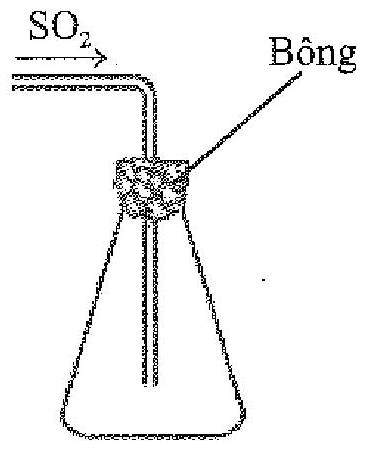
\includegraphics[max width=\textwidth, center]{2025_10_23_fa9073eecee116ad8cf2g-24}\\
7.16. Sau khi điều chế, khí $\mathrm{SO}_{2}$ có lẫn hơi nước được dẫn qua bình làm khô chứa các hạt chất rắn T rồi thu vào bình chựa theo hình vẽ sau:\\
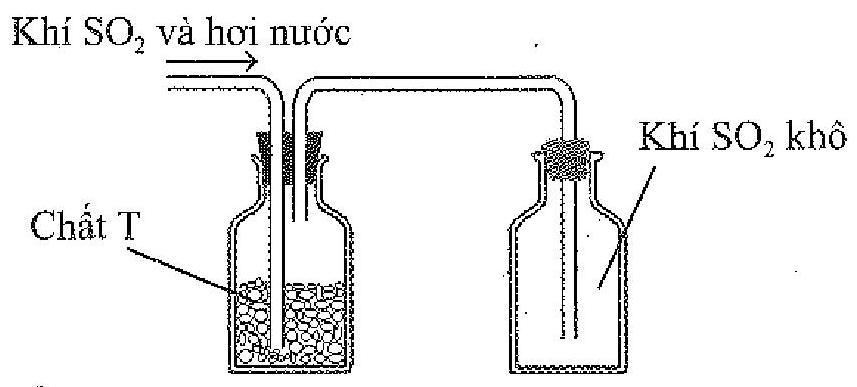
\includegraphics[max width=\textwidth, center]{2025_10_23_fa9073eecee116ad8cf2g-24(1)}

Chất T có thể là\\
A. KOH .\\
B. NaOH .\\
C. CaO .\\
D. $\mathrm{P}_{2} \mathrm{O}_{5}$.\\
7.17. Xét phản úng giữa sulfur và hydrogen ở điều kiện chuẩn:\\
$\mathrm{H}_{2}(\mathrm{~g})+\frac{1}{8} \mathrm{~S}_{8}(\mathrm{~s}) \longrightarrow \mathrm{H}_{2} \mathrm{~S}(\mathrm{~g}) \quad \Delta_{\mathrm{r}} \mathrm{H}_{298}^{\mathrm{o}}=-20,6 \mathrm{~kJ}$\\
Nhiệt tạo thành của $\mathrm{H}_{2} \mathrm{~S}(\mathrm{~g})$ là\\
A. $-20,6 \mathrm{~kJ} / \mathrm{mol}$.\\
B. $-41,2 \mathrm{~kJ} / \mathrm{mol}$.\\
C. $41,2 \mathrm{~kJ} / \mathrm{mol}$.\\
D. $20,6 \mathrm{~kJ} / \mathrm{mol}$.\\
7.18. Cho các ứng dụng sau:\\
(1) sản xuất sulfuric acid;\\
(2) tẩy trắng bột giấy;\\
(3) diệt nấm mốc, thuốc đông $y$;\\
(4) diệt trùng nước sinh hoạt.

Số ứng dụng của khí sulfur dioxide trong đời sông, sản xuất là\\
A. 1 .\\
B. 2 .\\
C. 3 .\\
D. 4 .\\
7.19. Sulfur và quặng pyrite sắt là các nguyên liệu chính trong công nghiệp sản xuất sulfuric acid.\\
Tại một nhà máy, cư đốt cháy 1 tấn quặng pyrite sắt (chưa $84 \%$ khối lượng $\mathrm{FeS}_{2}$ ) bằng không khí, thu được tói đa $\mathrm{V} \mathrm{m}^{3} \mathrm{khí} \mathrm{SO}_{2}$ (đkc). Giá trị cúa V là\\
A. 173,5 .\\
B. 347,0 .\\
C. 86,8 .\\
D. 477,2 .\\
7.20. Phản ứng chuyển hoá hydrogen sulfide trong khí thiên nhiên thành sulfur được thực hiện theo so đồ phản ứng:\\
$\mathrm{H}_{2} \mathrm{~S}+\mathrm{SO}_{2} \longrightarrow \mathrm{~S}+\mathrm{H}_{2} \mathrm{O}$\\
Khối lượng sulfur tối đa tạo ra khi chuyển hoá $1000 \mathrm{~m}^{3}$ khí thiên nhiên (đkc) (chứa $5 \mathrm{mg} \mathrm{H}_{2} \mathrm{~S} / \mathrm{m}^{3}$ ) là\\
A. $10,0 \mathrm{~g}$.\\
B. $5,0 \mathrm{~g}$.\\
C. $7,06 \mathrm{~g}$.\\
D. $100,0 \mathrm{~g}$.

\section*{VAN DUNG}
7.21. Sự phự thuộc của độ tan khí sulfur dioxide trong nước vào nhiệt độ được mô tả ở đồ thị bên.\\
Dựa vào đồ thị, hãy ước tính:\\
a) Dộ tan của sulfur dioxide ờ $20^{\circ} \mathrm{C}$. Nhận xét về tính tan của sulfur dioxide ở nhiệt độ này.\\
b) Nồng độ phần trăm của đung dịch sulfur dioxide bão hoà ở $20^{\circ} \mathrm{C}$.\\
c) Nhiệt độ tại đó độ tan của khí sulfur dioxide là 10 g trong 100 g nước.

\begin{figure}[h]
\begin{center}
  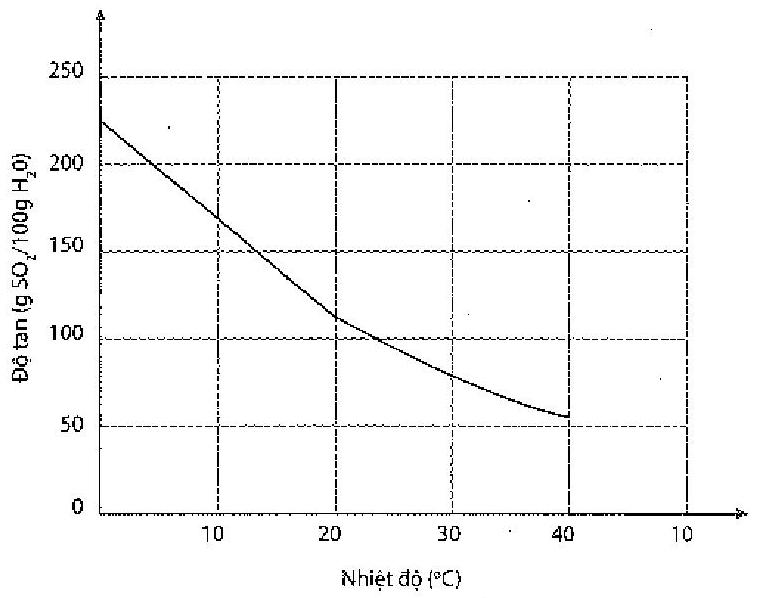
\includegraphics[width=\textwidth]{2025_10_23_fa9073eecee116ad8cf2g-25}
\captionsetup{labelformat=empty}
\caption{Sư phu thuộc cưa độ tan khi sulfur dioxide vào nhiệt độ}
\end{center}
\end{figure}

7.22. Phản úng oxi hoá $\mathrm{SO}_{2}$ là giai đoạn then chốt trong quá trình sản xuất $\mathrm{H}_{2} \mathrm{SO}_{4}$ : $\mathrm{SO}_{2}(\mathrm{~g})+\frac{1}{2} \mathrm{O}_{2}(\mathrm{~g}) \rightleftharpoons \mathrm{SO}_{3}(\mathrm{~g}) \quad \Delta_{\mathrm{r}} \mathrm{H}_{298}^{\mathrm{o}}=-99,2 \mathrm{~kJ}$\\
a) Viết biểu thức tính hằng số cân bằng $K_{C}$ của phản ứng.\\
b) Hãy cho biết phản ứng trên là toả nhiệt hay thu nhiệt.\\
c) Trong thực tế, phản úng được thực hiện ở khoảng $450^{\circ} \mathrm{C}$. Tại sao không thực hiện phản úng ờ $25^{\circ} \mathrm{C}$ hoặc $600^{\circ} \mathrm{C}$ ?\\
7.23. Xét phản ứng giữa $\mathrm{NO}_{2}$ và $\mathrm{SO}_{2}$ trong không khí ô nhiễm sulfur dioxide:\\
$\mathrm{NO}_{2}(\mathrm{~g})+\mathrm{SO}_{2}(\mathrm{~g}) \longrightarrow \mathrm{NO}(\mathrm{g})+\mathrm{SO}_{3}(\mathrm{~g})$\\
Tính biến thiên enthalpy của phản ứng và cho biết phản ứng trên là toả nhiệt hay thu nhiệt. (Biết nhiệt tạo thành của $\mathrm{NO}_{2}(\mathrm{~g}), \mathrm{SO}_{2}(\mathrm{~g}), \mathrm{NO}(\mathrm{g})$ và $\mathrm{SO}_{3}(\mathrm{~g})$ lần lượt là $33,2 \mathrm{~kJ} / \mathrm{mol},-296,8 \mathrm{~kJ} / \mathrm{mol}, 91,3 \mathrm{~kJ} / \mathrm{mol}$ và $-395,7 \mathrm{~kJ} / \mathrm{mol}$.)\\
7.24. Hỗn hợp X gồm $\mathrm{SO}_{2}$ và $\mathrm{O}_{2}$ có tỉ khối so với $\mathrm{H}_{2}$ bằng 24. Nung nóng X trong bình kín chưa xúc tác $\mathrm{V}_{2} \mathrm{O}_{5}$, thu được hỗn hợp khí Y có ti khối so với $\mathrm{H}_{2}$ bằng 30. Viết phương trình hoá học và tính hiệu suât của phản ứng oxi hoá $\mathrm{SO}_{2}$ thành $\mathrm{SO}_{3}$.\\
7.25. Tai nhiều làng nghề thủ công mî nghệ, sulfur dioxide được dùng là chất chống mốc cho các sản phẩm mây tre đan.\\
Trong một ngày, một làng nghề đốt cháy 20 kg sulfur để tạo thành sulfur dioxide.\\
a) Viết phương trình hoá học và tính thể tích khi $\mathrm{SO}_{2}$ (đkc) tối đa tạo ra?\\
b) Giả thiết có $20 \%$ lượng khí $\mathrm{SO}_{2}$ trên bay vào khí quyển và chuyển hoá hết thành $\mathrm{H}_{2} \mathrm{SO}_{4}$ trong nước mưa theo sơ đồ:\\
$\mathrm{SO}_{2} \xrightarrow[\mathrm{xt}]{+\mathrm{O}_{2}} \mathrm{SO}_{3} \xrightarrow{+\mathrm{H}_{2} \mathrm{O}} \mathrm{H}_{2} \mathrm{SO}_{4}$

\begin{itemize}
  \item Viết các phương trình hoá học theo so đồ trến.
  \item Tính thể tích nước mưa bị nhiểm acid nếu nồng độ $\mathrm{H}_{2} \mathrm{SO}_{4}$ trong nước mura là $1,25 \cdot 10^{-5} \mathrm{M}$.
\end{itemize}

\section*{BÀI 8}
\section*{SULFURIC ACID VÀ MUỐI SULFATE}
\section*{NHANT BIET}
8.1. Sulfuric acid đựng trong chai thuỷ tinh thường được bán trên thị trường có nồng độ là\\
A. $98 \%$.\\
B. $36 \%$.\\
C. $63 \%$.\\
D. $8 \%$.\\
8.2. Dung dịch acid nào sau đây có khả năng gây bỏng nếu rơi vào da?\\
A. $\mathrm{HCl} 36 \%$.\\
B. $\mathrm{HNO}_{3} 63 \%$.\\
C. $\mathrm{H}_{2} \mathrm{SO}_{4} 98 \%$.\\
D. $\mathrm{H}_{3} \mathrm{PO}_{4} 85 \%$.\\
8.3. Chất nào sau đây không bay hơi ở điều kiện thương do có nhiệt độ sôi rât cao $\left(337^{\circ} \mathrm{C}\right)$ ?\\
A. $\mathrm{H}_{2} \mathrm{O}$.\\
B. $\mathrm{HNO}_{3}$.\\
C. $\mathrm{NH}_{3}$.\\
D. $\mathrm{H}_{2} \mathrm{SO}_{4}$.\\
8.4. Quá trình pha loãng dung dịch đậm đặc của acid nào sau đây toả rất nhiều nhiệt nên không đưọc tự ý pha loãng?\\
A. HCl .\\
B. $\mathrm{H}_{2} \mathrm{SO}_{4}$.\\
C. $\mathrm{CH}_{3} \mathrm{COOH}$.\\
D. $\mathrm{HNO}_{3}$.\\
8.5. Ở thể lỏng, chất nào sau đây có dang sánh như dầu do tồn tại liên kết hydrogen rât mạnh giữa các phân tư?\\
A. HF.\\
B. $\mathrm{H}_{2} \mathrm{SO}_{4}$.\\
C. $\mathrm{H}_{2} \mathrm{O}$.\\
D. $\mathrm{CH}_{3} \mathrm{COOH}$.\\
8.6. Bưóc sơ cứu đầu tiên cần làm ngay khi một người bị bỏng sulfuric acid là\\
A. rưa với nước lạnh nhiều lần.\\
B. trung hoà acid bằng $\mathrm{NaHCO}_{3}$.\\
C. băng bó tạm thời vết bỏng.\\
D. đưa đến cơ sở y tế gần nhất.\\
8.7. Trong công nghiêp, hydrogen fluoride được điều chế từ quặng fluorite theo phản úmg: $\mathrm{CaF}_{2}+\mathrm{H}_{2} \mathrm{SO}_{4} \xrightarrow{250^{\circ} \mathrm{C}} \mathrm{CaSO}_{4}+2 \mathrm{HF}$\\
Vai trò của sulfuric acid trong phản ứng là\\
A. base.\\
B. chất oxi hoá.\\
C. acid.\\
D. chất khử.\\
8.8. Sulfuric acid đặc thể hiện tính chất nào khi lấy nước từ hợ chất carbohydrate và khiến chúng hoá đen?\\
A. Tính acid.\\
B. Tinh base.\\
C. Tính háo nước.\\
D. Tính dễ tan.\\
8.9. Phân biệt đưọc dung dịch $\mathrm{Na}_{2} \mathrm{SO}_{4}$ và NaCl bằng dung dịch nào sau đây?\\
A. $\mathrm{MgCl}_{2}$.\\
B. $\mathrm{FeCl}_{2}$.\\
C. HCl .\\
D. $\mathrm{BaCl}_{2}$.\\
8.10. Muối X không tan trong nước và các dung môi hữu co. Trong y học, X thường được dùng làm chất cản quang trong xét nghiệm X-quang đường tiêu hoá. Công thức của X là\\
A. $\mathrm{BaSO}_{4}$.\\
B. $\mathrm{Na}_{2} \mathrm{SO}_{4}$.\\
C. $\mathrm{K}_{2} \mathrm{SO}_{4}$.\\
D. $\mathrm{MgSO}_{4}$.

\section*{THONG HISU}
8.11. Trong công nghiệp sản xuất sulfuric acid, hai nguồn nguyên liệu được khai thác từ mỏ để cung cấp nguyên tố lưu huỳnh là\\
A. $\mathrm{ZnS}, \mathrm{PbS}$.\\
B. $\mathrm{H}_{2} \mathrm{~S}, \mathrm{SO}_{2}$.\\
C. $\mathrm{CaSO}_{4}, \mathrm{BaSO}_{4}$.\\
D. $\mathrm{S}, \mathrm{FeS}_{2}$.\\
8.12. Khi trộn dung dịch $\mathrm{Na}_{2} \mathrm{SO}_{4}$ với dung dịch $\mathrm{BaCl}_{2}$, phản ứng thực chất xảy ra trong dung dịch là\\
A. $\mathrm{Ba}^{2+}+\mathrm{SO}_{4}^{2-} \longrightarrow \mathrm{BaSO}_{4}$.\\
B. $\mathrm{Na}^{+}+\mathrm{Cl}^{-} \longrightarrow \mathrm{NaCl}$.\\
C. $\mathrm{Ba}^{2+}+\mathrm{Na}_{2} \mathrm{SO}_{4} \longrightarrow \mathrm{BaSO}_{4}+2 \mathrm{Na}^{+}$.\\
D. $\mathrm{BaCl}_{2}+\mathrm{SO}_{4}^{2-} \longrightarrow \mathrm{BaSO}_{4}+2 \mathrm{Cl}^{-}$.\\
8.13. Quá trình sản xuất sulfuric acid trong công nghiệp được thực hiện dựa trên các phản ứng sau:\\
(a) $\mathrm{S}+\mathrm{O}_{2} \xrightarrow{\mathrm{t}^{\circ}} \mathrm{SO}_{2}$\\
(b) $4 \mathrm{FeS}_{2}+11 \mathrm{O}_{2} \xrightarrow{\mathrm{t}^{\mathrm{a}}} 2 \mathrm{Fe}_{2} \mathrm{O}_{3}+8 \mathrm{SO}_{2}$\\
(c) $2 \mathrm{SO}_{2}+\mathrm{O}_{2} \underset{\mathrm{t}^{\mathrm{a}}}{\stackrel{\mathrm{V}_{2} \mathrm{O}_{5}}{\rightleftharpoons}} 2 \mathrm{SO}_{3}$\\
(d) $\mathrm{H}_{2} \mathrm{SO}_{4}+\mathrm{SO}_{3} \longrightarrow \mathrm{H}_{2} \mathrm{~S}_{2} \mathrm{O}_{7}$

Số phản ứng xảy ra đồng thời quá trình oxi hoá và quá trình khử là\\
A. 1 .\\
B. 3 .\\
C. 2 .\\
D. 4 .\\
8.14. Cho nhiệt tạo thành chuẩn của $\mathrm{SO}_{2}(\mathrm{~g})$ và $\mathrm{SO}_{3}(\mathrm{~g})$ lần lượt là $-296,8 \mathrm{~kJ} / \mathrm{mol}$ và $-395,7 \mathrm{~kJ} / \mathrm{mol}$.\\
Biến thiên enthalpy chuẩn của phản ứng: $2 \mathrm{SO}_{2}+\mathrm{O}_{2} \xlongequal[\mathrm{t}^{\circ}]{\mathrm{V}_{2} \mathrm{O}_{5}} 2 \mathrm{SO}_{3}$ là\\
A. $-98,9 \mathrm{~kJ}$.\\
B. $-197,8 \mathrm{~kJ}$.\\
C. $98,9 \mathrm{~kJ}$.\\
D. $197,8 \mathrm{~kJ}$.\\
8.15. Cho dung dịch sulfuric acid đặc tác dụng với từng chất rắn sau: $\mathrm{NaCl}, \mathrm{NaBr}$, $\mathrm{NaI}, \mathrm{NaHCO}_{3}$ ở nhiệt độ thường.\\
Số phản ứng trong đó sulfuric acid đóng vai trò chất oxi hoá là\\
A. 2 .\\
B. 4 .\\
C. 1 .\\
D. 3 .\\
8.16. Cho các họp chất carbohydrate sau: đường glucose, đường saccharose, bong, bột gỗ.\\
Số hợp chất có khả năng bị hoá đen khi tiếp xúc với sulfuric acid đặc là\\
A. 1 .\\
B. 2 .\\
C. 3.\\
D. 4 .\\
8.17. Trong công nghiệp sản xuất sulfuric acid, sulfur trioxide được hấp thụ vào dung dịch sulfuric acid đặc tạo thành nhưng hợp chất có công thúc chung là\\
A. $\mathrm{H}_{2} \mathrm{~S}_{2} \mathrm{O}_{7}$.\\
B. $\mathrm{H}_{2} \mathrm{SO}_{4}$.\\
C. $\mathrm{H}_{2} \mathrm{SO}_{4} \cdot \mathrm{nSO}_{3}$.\\
D. $\left(\mathrm{SO}_{3}\right)_{\mathrm{n}}$.\\
8.18. Cho các nguyên liệu sau: sulfur, quặng pyrite ( FeS 2 ), không khí, nước, vanadium(V) oxide $\left(\mathrm{V}_{2} \mathrm{O}_{5}\right)$.\\
Số nguyên liệu được sử dụng trong công nghiệp sản xuất sulfuric acid là\\
A. 4 .\\
B. 2 .\\
C. 5 .\\
D. 3 .\\
8.19. Kết quả phân tích thành phần một muối sulfate cho thấy nguyên tố kim loại M chiếm 28\% về khối lượng, còn lại là oxygen và lưu huỳnh. Kím loại M là\\
A. Fe.\\
B. Cu .\\
C. Mg.\\
D. Ca.\\
8.20. Hoà tan hết $m$ gam oxide của kim loại $M$ (hoá trị II) vào dung dịch $\mathrm{H}_{2} \mathrm{SO}_{4}$ loãng, thu được 3m gam muối sulfate. Công thức của oxide kim loại là\\
A. ZnO .\\
B. CuO.\\
C. CaO .\\
D. MgO .

\section*{VAN DUNG}
8.21. Cho vào hai ống nghiệm, mỗi ống $20,00 \mathrm{~mL}$ dung dịch X gồm các ion sau: $\mathrm{Mg}^{2+}, \mathrm{NH}_{4}^{+}, \mathrm{SO}_{4}^{2-}$ và $\mathrm{Cl}^{-}$.\\
Cho dung dịch NaOH dư vào ống nghiệm thứ nhất, đun nóng, thu được $0,116 \mathrm{~g}$ kết tủa và $49,58 \mathrm{~mL}$ khí (đlkc).\\
Cho dung dịch $\mathrm{BaCl}_{2}$ dư vào ống nghiệm thứ hai, thu được $0,233 \mathrm{~g}$ kết tủa. Xác định nồng độ mol mỗi loại ion trong dung dịch X.\\
8.22. Trong công nghiệp, copper(II) sulfate được sản xuất bằng cách ngâm đồng phế liệu trong sulfuric acid loãng và sục không khí:


\begin{equation*}
\mathrm{Cu}+\mathrm{O}_{2}+\mathrm{H}_{2} \mathrm{SO}_{4} \text { (loãng) } \longrightarrow \mathrm{CuSO}_{4}+\mathrm{H}_{2} \mathrm{O} \tag{1}
\end{equation*}


a) Lập phương trình hoá học của phản ứng (1).\\
b) Tại sao thực tế không sản xuất $\mathrm{CuSO}_{4}$ từ đồng phế liệu theo so đồ phản ứng:


\begin{equation*}
\mathrm{Cu}+\mathrm{H}_{2} \mathrm{SO}_{4}(\text { đặc }) \xrightarrow{\mathrm{t}^{\circ}} \mathrm{CuSO}_{4}+\mathrm{SO}_{2}+\mathrm{H}_{2} \mathrm{O} \tag{2}
\end{equation*}


8.23. Sulfur dioxide là một trong các tác nhân gây mưa acid, phát thải chủ yếu từ các quá trình đốt cháy nhiên liệu như than đá, xăng, dầu,...\\
Một nhà máy nhiệt điện than sử dụng hết 6000 tấn than đá/ngày, có thành phần chưa $0,8 \%$ lưu huỳnh về khối lượng để làm nhiên liệu.\\
a) Tính thể tích khí $\mathrm{SO}_{2}$ (đkc) tối đa do nhà máy tạo ra trong một ngày.\\
b) Giả thiết có $1 \%$ lượng khí $\mathrm{SO}_{2}$ tạo ra khuếch tán vào khí quyển rồi bị chuyển hoá thành sulfuric acid trong nước mưa theo so đồ:\\
$\mathrm{SO}_{2} \xrightarrow[\text { xt }]{+\mathrm{O}_{2}} \mathrm{SO}_{3} \xrightarrow{+\mathrm{H}_{2} \mathrm{O}} \mathrm{H}_{2} \mathrm{SO}_{4}$\\
Tính thể tích nước mưa bị nhiểm acid, giả thiết nồng độ sulfuric acid trong nước mưa là $1 \cdot 10^{-5} \mathrm{M}$.\\
8.24. Trong sản xuất phân bón, surpephosphate kép chứa thành phần dinh dưỡng là $\mathrm{Ca}\left(\mathrm{H}_{2} \mathrm{PO}_{4}\right)_{2}$, được sản xuất từ quặng phosphorite theo hai giai đoạn sau:\\
$\mathrm{Ca}_{3}\left(\mathrm{PO}_{4}\right)_{2}+3 \mathrm{H}_{2} \mathrm{SO}_{4} \longrightarrow 2 \mathrm{H}_{3} \mathrm{PO}_{4}+3 \mathrm{CaSO}_{4}$\\
$\mathrm{Ca}_{3}\left(\mathrm{PO}_{4}\right)_{2}+4 \mathrm{H}_{3} \mathrm{PO}_{4} \longrightarrow 3 \mathrm{Ca}\left(\mathrm{H}_{2} \mathrm{PO}_{4}\right)_{2}$\\
Để sản xuất được 1 tấn $\mathrm{Ca}\left(\mathrm{H}_{2} \mathrm{PO}_{4}\right)_{2}$ với hiệu suất của cả quá trình là $80 \%$ thì cần bao nhiêu tấn dung dịch $\mathrm{H}_{2} \mathrm{SO}_{4} 70 \%$ ?

\section*{BÀI 9}
\section*{ÔN TÂP CHUONG 2}
\section*{NHAN BIET}
9.1. Trong khí quyển Trái Đất, phần trăm thể tích khí nitrogen chiếm là\\
A. $21 \%$.\\
B. $1 \%$.\\
C. $78 \%$.\\
D. $28 \%$.\\
9.2. Chất nào sau đây được sử dựng là chất làm lạnh trong các hệ thông làm lạnh công nghiệp?\\
A. $\mathrm{N}_{2}$.\\
B. $\mathrm{NH}_{3}$.\\
C. $\mathrm{SO}_{2}$.\\
D. S.\\
9.3. Mưa acid là một thảm hoą thiên nhiên toàn cầu, ảnh hưởng đến sự sống của các sinh vật. Mưa acid là hiện tượng nước mưa có pH\\
A. $<5,6$.\\
B. $=7$.\\
C. 6-7.\\
D. $>8$.\\
9.4. Quá trình đốt cháy hỗn hợp hơi nhiên liệu và không khí trong động co khi đánh tia lửa điện sinh ra khí NO, một tác nhân gây ô nhiễm không khí. Tên gọi của NO là\\
A. ammonia.\\
B. nitrogen dioxide.\\
C. nitrogen monoxide.\\
D. nitrogen.\\
9.5. Oxide $X$ là chất khí, mùi hắc, độc (gây ho, viêm đương hô hấp). Trong công nghiêp, $X$ được dừng làm chất tẩy trắng bột gỗ, sản xuất sulfuric acid. Công thức của X là\\
A. $\mathrm{CO}_{2}$.\\
B. $\mathrm{H}_{2} \mathrm{~S}$.\\
C. $\mathrm{SO}_{2}$.\\
D. $\mathrm{P}_{2} \mathrm{O}_{5}$.\\
9.6. Nhỏ 1 giot dung dịch acid đặc nào sau đây lên tờ giấy trắng thì tờ giấy bị hoá đen ở chỗ tiếp xúc với acid?\\
A. HBr .\\
B. HCl .\\
C. $\mathrm{HNO}_{3}$.\\
D. $\mathrm{H}_{2} \mathrm{SO}_{4}$.\\
9.7. Dung dịch loãng của acid nào sau đây hoà tan được lá bạc, tạo thành muối tưong úng?\\
A. $\mathrm{HNO}_{3}$.\\
B. HCl .\\
C. $\mathrm{H}_{3} \mathrm{PO}_{4}$.\\
D. $\mathrm{H}_{2} \mathrm{SO}_{4}$.\\
9.8. Trong công nghiệp, quặng pyrite sắt ( $\mathrm{FeS}_{2}$ ) được dùng làm nguyên liệu để\\
A. luyện gang.\\
B. sản xuất sulfuric acid.\\
C. chế tạo nam châm điện.\\
D. tổng hợ dược phẩm.\\
9.9. Khí nào sau đây tan trong nước thu được dung dịch có khả năng làm phenolphthalein chuyển màu hồng?\\
A. Nitrogen.\\
B. Ammonia.\\
C. Sulfur dioxide.\\
D. Hydrogen chloride.

\section*{THONG HISU}
9.10. Trong công nghiệp thực phẩm, nitrogen lỏng $(\mathrm{D}=0,808 \mathrm{~g} / \mathrm{mL})$ được phun vào vỏ bao bì trước khi đóng nắp để làm căng vỏ bao bì.\\
Thể tích khí nitrogen thu được (đkc) khi hoá hơi 1 mL nitrogen lỏng là\\
A. $646,4 \mathrm{~mL}$.\\
B. $808,0 \mathrm{~mL}$.\\
C. $715,4 \mathrm{~mL}$.\\
D. $1095,7 \mathrm{~mL}$.\\
9.11. Cho cân bằng hoá học sau: $\mathrm{N}_{2}(\mathrm{~g})+3 \mathrm{H}_{2}(\mathrm{~g}) \rightleftharpoons 2 \mathrm{NH}_{3}(\mathrm{~g}) \quad \Delta_{\mathrm{r}} \mathrm{H}_{298}^{\mathrm{o}}<0$ Tổng số mol của hỗn hợp khí khi hệ đạt cân bằng ở nhiệt độ $400^{\circ} \mathrm{C}$ và $500^{\circ} \mathrm{C}$ lần lượt bằng x và y . Mối quan hệ giữa x và y là\\
A. $x>y$.\\
B. $x=y$.\\
C. $x<y$.\\
D. $5 x=4 y$.\\
9.12. Cho một ít tinh thể muối X vào ống nghiệm và đụn nóng trên ngọn lửa đèn cồn, sau một thời gian thấy không còn chất rắn nào ở đáy ống nghiệm. Muối X có thể là muối nào sau đây?\\
A. NaCl .\\
B. $\mathrm{CaCO}_{3}$.\\
C. $\mathrm{KClO}_{3}$.\\
D. $\mathrm{NH}_{4} \mathrm{Cl}$.\\
9.13. Cho các chất sau: $\mathrm{H}_{2} \mathrm{SO}_{4}, \mathrm{SO}_{2}, \mathrm{~N}_{2}, \mathrm{NH}_{3}$.

Số chất tan tốt trong nước ở điều kiện thường là\\
A. 4 .\\
B. 1 .\\
C. 3 .\\
D. 4 .\\
9.14. Trong phản ứng giữa khí ammonia và khí hydrogen chloride tạo thành ammonium chloride ở dạng khói trắng, ammonia dóng vai trò là\\
A. acid.\\
B. base.\\
C. chất oxi hoá.\\
D. chất khử.\\
9.15. Cho các acid ở dạng đậm đặc sau: $\mathrm{HCl}, \mathrm{HNO}_{3}, \mathrm{H}_{3} \mathrm{PO}_{4}, \mathrm{H}_{2} \mathrm{SO}_{4}$.

Số acid vừa có tính acid mạnh, vừa có tính oxi hoá mạnh là\\
A. 1 .\\
B. 4 .\\
C. 3 .\\
D. 2 .\\
9.16. Tiến hành các thí nghiệm cho dung dịch $\mathrm{H}_{2} \mathrm{SO}_{4}$ loãng lần lượt tác dụng với: $\mathrm{Mg}, \mathrm{NaHCO}_{3}, \mathrm{BaCl}_{2}, \mathrm{CaCO}_{3}$. Số thí nghiệm xảy ra phản ứng oxi hoá - khử là\\
A. 1 .\\
B. 2 .\\
C. 3 .\\
D. 4 .\\
9.17. Cho các chất khí sau: $\mathrm{H}_{2} \mathrm{~S}, \mathrm{NO}, \mathrm{NO}_{2}, \mathrm{SO}_{2}$.

Số khí gây ô nhiễm môi trường khi phát thải vào không khí là\\
A. 1 .\\
B. 4.\\
C. 3 .\\
D. 2 .\\
9.18. Cho cân bằng hoá học sau: $2 \mathrm{SO}_{2}(\mathrm{~g})+\mathrm{O}_{2}(\mathrm{~g}) \rightleftharpoons 2 \mathrm{SO}_{3}(\mathrm{~g}) \quad \Delta \mathrm{H}<0$ Khi tăng nhiệt độ,\\
A. tổng số mol khí trong hệ giảm.\\
B. hiệu suất phản ứng tăng.\\
C. cân bằng chuyển dịch theo chiều nghịch.\\
D. nồng độ khí sản phẩm tăng.\\
9.19. Một nhà máy luyện kim, ở giai đoạn đầu của quá trình sản xuất Zn từ quặng blend thu được sản phẩm phụ là $\mathrm{SO}_{2}$ theo so đồ phản ứng:\\
$\mathrm{ZnS}+\mathrm{O}_{2} \longrightarrow \mathrm{ZnO}+\mathrm{SO}_{2}$\\
Đốt cháy 1 tấn quặng blend (chưa $77,6 \%$ khối lượng ZnS ) bằng không khí, thu được tối đa $\mathrm{V} \mathrm{m}^{3}$ khí $\mathrm{SO}_{2}$ (đkc). Giá trị của V là\\
A. 992 .\\
B. 198,3 .\\
C. $297,5$.\\
D. 396,6 .

\section*{VAN DUNG}
9.20. Cho cân bằng hoá học sau: $2 \mathrm{NO}_{2}(\mathrm{~g}) \rightleftharpoons \mathrm{N}_{2} \mathrm{O}_{4}(\mathrm{~g})$\\
a) Hãy tính $\Delta_{\mathrm{I}} \mathrm{H}_{298}^{\mathrm{o}}$ của phản úng, cho nhiệt tạo thành của $\mathrm{NO}_{2}(\mathrm{~g})$ và $\mathrm{N}_{2} \mathrm{O}_{4}(\mathrm{~g})$ lần lượt là $33,2 \mathrm{~kJ} / \mathrm{mol}$ và $11,1 \mathrm{~kJ} / \mathrm{mol}$.\\
b) Cân bằng sẽ chuyển dịch theo chiều nào khi giảm nhiệt độ của hệ?\\
9.21. Hoà tan $3,92 \mathrm{~g}$ một muối X ngậm nước vào cốc nước, thu được 100 mL dung dịch X gồm các ion: $\mathrm{Fe}^{2+}, \mathrm{NH}_{4}^{+}$và $\mathrm{SO}_{4}^{2-}$. Cho dung dịch NaOH dư vào 20 mL dung dịch X , đun nóng, thu được $49,58 \mathrm{~mL}$ khí (đkc). Cho dung dich $\mathrm{BaCl}_{2}$ dư vào 20 mL dung dịch X , thu được $0,466 \mathrm{~g}$ kết tủa. Xác định công thức của X .\\
9.22. Cho phản úng sau:\\
$\mathrm{H}_{2}(\mathrm{~g})+\frac{1}{8} \mathrm{~S}_{8}(\mathrm{~g}) \longrightarrow \mathrm{H}_{2} \mathrm{~S}(\mathrm{~g}) \quad \Delta_{\mathrm{r}} \mathrm{H}_{298}^{\circ}=?$\\
Hãy xác định :\\
a) Biến thiên enthalpy $\Delta_{\mathrm{r}} \mathrm{H}_{298}^{\mathrm{o}}$ của phản ứng, cho nhiệt tạo thành chuẩn của $\mathrm{S}_{8}(\mathrm{~g})$ và $\mathrm{H}_{2} \mathrm{~S}(\mathrm{~g})$ lần lượt là $101,3 \mathrm{~kJ} / \mathrm{mol}$ và $-20,6 \mathrm{~kJ} / \mathrm{mol}$.\\
b) Năng lượng liên kết $\mathrm{S}-\mathrm{S}$ trong phân tử $\mathrm{S}_{8}(\mathrm{~g})$, biết $\mathrm{E}_{\mathrm{b}(\mathrm{H}-\mathrm{H})}=436 \mathrm{~kJ} / \mathrm{mol}$ và $\mathrm{E}_{\mathrm{b}(\mathrm{S}-\mathrm{H})}=363 \mathrm{~kJ} / \mathrm{mol}$.\\
9.23. Hydrogen sulfide phân huỷ theo phản ứng sau đây:\\
$2 \mathrm{H}_{2} \mathrm{~S}(\mathrm{~g}) \rightleftharpoons 2 \mathrm{H}_{2}(\mathrm{~g})+\mathrm{S}_{2}(\mathrm{~g})$\\
Hà̀ng số cân bằng $\mathrm{K}_{\mathrm{C}}=9,30 \cdot 10^{-8} \stackrel{\circ}{0}^{\circ} 427^{\circ} \mathrm{C}$.\\
a) Viết biểu thức hằng số cân bằng $K_{C}$ của phản ứng.\\
b) Xác định biến thiên enthalpy chuẩn của phản ứng, biết nhiệt tạo thành chuẩn của $\mathrm{H}_{2} \mathrm{~S}(\mathrm{~g})$ và $\mathrm{S}_{2}(\mathrm{~g})$ lần lượt là $-20,6 \mathrm{~kJ} / \mathrm{mol}$ và $128,6 \mathrm{~kJ} / \mathrm{mol}$. Cho biết phản ứng thuận là toả nhiệt hay thu nhiệt.\\
c) Ở $427^{\circ} \mathrm{C}$, tính hằng số cân bằng $\mathrm{K}^{\prime}{ }_{\mathrm{C}}$ của phản úng:\\
$2 \mathrm{H}_{2}(\mathrm{~g})+\mathrm{S}_{2}(\mathrm{~g}) \rightleftharpoons 2 \mathrm{H}_{2} \mathrm{~S}(\mathrm{~g})$\\
9.24. Hiện nay, mua acid, hiêu úng nhà kính và thủng tầng ozone là ba thảm hoạ môi trường toàn cầu. Mưa acid tàn phá nhiều rừng cây, các công trình kiến trúc bằng đá và kim loại. Tác nhân chủ yếu gây ra mưa acid là sulfur dioxide.\\
a) Trong khí quyển, $\mathrm{SO}_{2}$ chuyển hoá thành $\mathrm{H}_{2} \mathrm{SO}_{4}$ trong nươc mưa theo so đồ sau:\\
$\mathrm{SO}_{2} \xrightarrow[\mathrm{xt}]{+\mathrm{O}_{2}} \mathrm{SO}_{3} \xrightarrow{+\mathrm{H}_{2} \mathrm{O}} \mathrm{H}_{2} \mathrm{SO}_{4}$\\
Viết các phương trình hoá học.\\
b) Một cơn mưa acid xuất hiện tại một khu công nghiệp diện tích $10 \mathrm{~km}^{2}$ với lượng mưa trung bình 80 mm . Hãy tính:

\begin{itemize}
  \item Thể tích nước mưa đã rơi xuống khu công nghiệp.
  \item Khối lượng $\mathrm{H}_{2} \mathrm{SO}_{4}$ trong lượng nước mưa, biết nồng độ $\mathrm{H}_{2} \mathrm{SO}_{4}$ trong nước mưa là $2 \cdot 10^{-5} \mathrm{M}$.\\
c) Lượng acid trong nước mưa có thể ăn mòn các công trình bằng đá vôi.
  \item Viết 1 phương trình hoá học minh hoạ.
  \item Khối lượng $\mathrm{CaCO}_{3}$ tối đa bị ăn mòn bởi lượng acid trên.\\
d) Em hãy tìm hiểu về nguyên nhân phát sinh các khí gây mưa acid và đề xuất giải pháp hạn chế.
\end{itemize}

\section*{BÀ 10}
\section*{HỢP CHÁT HƯU CO VÀ HOÁ HOC HỮU CO}
\section*{NHAN BIET}
10.1. Hợp chất hữu co là các họp chất của ......... (trừ các oxide của carbon, muối carbonate, cyanide, carbide,...). Từ thich họp điền vào chỗ trống trong định nghĩa trên là\\
A. carbon.\\
B. hydrogen.\\
C. oxygen.\\
D. nitrogen.\\
10.2. Xét phản úng quang hợp: $6 \mathrm{CO}_{2}+6 \mathrm{H}_{2} \mathrm{O} \longrightarrow \mathrm{C}_{6} \mathrm{H}_{12} \mathrm{O}_{6}+6 \mathrm{O}_{2}$ Chất nào trong phản úng này thuộc loại họp chất hữu co?\\
A. $\mathrm{CO}_{2}$.\\
B. $\mathrm{H}_{2} \mathrm{O}$.\\
C. $\mathrm{C}_{6} \mathrm{H}_{12} \mathrm{O}_{6}$.\\
D. $\mathrm{O}_{2}$,\\
10.3. Hoá học hữu cơ là ngành hoá học chuyên nghiên cứu về các $\_\_\_\_$ Cụm từ thích hợp điền vào chỗ trống trong định nghĩa trên là\\
A. họp chất hữu co.\\
B. hợp chất vô co.\\
C. hợp chất thiên nhiên.\\
D. hợp chất phức.\\
10.4. Nhận xét nào dưới đây về đặc điểm chung của các chất hữu cơ không đúng?\\
A. Các hợp chất hữu cơ thường khó bay hơi, bền với nhiệt và khó cháy.\\
B. Liên kết hoá học chủ yếu trong các phân tử hợp chất hữu cơ là liên kết cộng hoá trị.\\
C. Các hợp chất hữu cơ thường khộng tan hoặc ît tan trong nước, tan trong dung môi hữu co.\\
D. Các phản ứng hoá học của hợp chất hữu cơ thường xảy ra chậm và theo nhiều hướng khác nhau tạo ra một hỗn họp các sản phẩm.\\
10.5. Hydrocarbon là loại hợp chất hữu cơ mà thành phần phân tứ có các nguyên tố nào sau đây?\\
A. C và H .\\
B. $\mathrm{C}, \mathrm{H}$ và O .\\
C. $\mathrm{C}, \mathrm{H}$ và N.\\
D. $\mathrm{C}, \mathrm{H}, \mathrm{O}$ và N.\\
10.6. Nhóm chức là ........ gây ra những phản ưng đặc trưng của phân tử họp chất hữu co. Cụm từ thích hợp điền vào chỗ trống trong phát biểu trên là\\
A. nguyên từ.\\
B. phân tứ.\\
C. nhóm nguyên tử.\\
D. nguyên tử hoặc nhóm nguyên tử.\\
10.7. Phổ hồng ngoai là phương pháp vật lí rất quan trọng và phổ biến để nghiên cứu về\\
A. thành phần nguyên tố chất hữu co.\\
B. thành phần phân tữ hợp chất hữu cơ.\\
C. cấu tạo hợp chất hữu co.\\
D. cấu trúc không gian hợp chất hữu co.

\section*{Fivitiong HILU}
10.8. Xét các chất $\mathrm{CH}_{4}, \mathrm{HCN}, \mathrm{CO}_{2}, \mathrm{CH}_{2}=\mathrm{CH}_{2}, \mathrm{CH}_{3} \mathrm{CH}=\mathrm{O}, \mathrm{Na}_{2} \mathrm{CO}_{3}, \mathrm{CH}_{3} \mathrm{COONa}$, $\mathrm{H}_{2} \mathrm{NCH}_{2} \mathrm{COOH}$ và $\mathrm{Al}_{4} \mathrm{C}_{3}$. Trong các chất này, số hợp chất hữu cơ là\\
A. 3 .\\
B. 4 .\\
C. 5.\\
D. 6 .\\
10.9. Phân tữ chất nào sau đây không chỉ chứa liên kết cộng hoá trị?\\
A. $\mathrm{CH}_{3} \mathrm{CH}_{2} \mathrm{OH}$.\\
B. $\mathrm{CH}_{3} \mathrm{CH}=\mathrm{O}$.\\
C. $\mathrm{CH} \equiv \mathrm{CH}$.\\
D. $\mathrm{CH}_{3} \mathrm{COONa}$.\\
10.10. Trong các chất sau đây, chất nào dễ cháy nhất?\\
A. $\mathrm{CO}_{2}$.\\
B. $\mathrm{C}_{2} \mathrm{H}_{5} \mathrm{OH}$.\\
C. $\mathrm{Na}_{2} \mathrm{CO}_{3}$.\\
D. $\mathrm{N}_{2}$.\\
10.11. Cho cảc hợp chất sau: $\mathrm{CH}_{4} ; \mathrm{NH}_{3} ; \mathrm{C}_{2} \mathrm{H}_{2} ; \mathrm{CCl}_{4} ; \mathrm{C}_{2} \mathrm{H}_{4} ; \mathrm{C}_{6} \mathrm{H}_{6}$. Số hợp chất thuộc loại hydrocarbon là\\
A. 1 .\\
B. 2 .\\
C. 3 .\\
D. 4 .\\
10.12. Biết rằng hydrocarbon no chỉ chúa liên kết đơn, hydrocarbon không no có chưa liên kết bội và hydrocarbon thơm có chứa vòng benzene. Xét các chất sau:\\
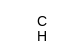
\includegraphics{smile-1705ef711880c333f350adac6534233da891a6d5}\\
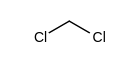
\includegraphics{smile-f9d0a229f3259a7f8f713a40058d6fc8510976a7}\\
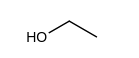
\includegraphics{smile-2977b4e51505100d21a20b04d7c9ad1091ed9cb3}\\
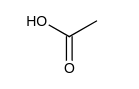
\includegraphics{smile-6394524a10b89e42a47e93f211cf05f3108d9dd3}\\
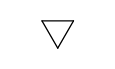
\includegraphics{smile-ad1e25332066f5859dedef005bb44a27eef79d45}\\
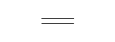
\includegraphics{smile-b7c819dea4ead953d2cd0f48eaf1542814857271}\\
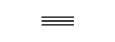
\includegraphics{smile-7f8e23ebccf6a7ce64347a8c830055147c99caf6}\\
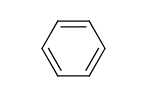
\includegraphics{smile-758f72acc6b1daf3f43294845632ae50fbc3c53c}

Nhận định nào sau đây không đúng?\\
A. Số hydrocarbon bằng 5.\\
B. Số dẫn xuất hydrocarbon bằng 3.\\
C. Số hydrocarbon no bằng 2.\\
D. Số hydrocarbon không no bằng 3.\\
10.13. Nhận định nào sau đây không đúng?\\
A. $\mathrm{CH}_{4}, \mathrm{CH}_{2}=\mathrm{CH}_{2}$ và $\mathrm{CH} \equiv \mathrm{CH}$ là những hydrocarbon.\\
B. $\mathrm{CH}_{3} \mathrm{OH}$ và $\mathrm{HOCH}_{2}-\mathrm{CH}_{2} \mathrm{OH}$ là những alcohol.\\
C. $\mathrm{CH}_{3} \mathrm{COOH}$ và $\mathrm{CH}_{2}(\mathrm{COOH})_{2}$ là những carboxylic acid.\\
D. $\mathrm{CH}_{3} \mathrm{CH}=\mathrm{O}$ và $\mathrm{CH}_{3} \mathrm{COCH}_{3}$ là những aldehyde.\\
10.14. Xét các chất sau:\\
$\mathrm{CH}_{3}-\mathrm{CH}_{2} \mathrm{OH}$\\
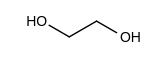
\includegraphics{smile-b319609c369ffca781d62511cb1af7a8bc77665b}\\
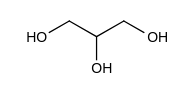
\includegraphics{smile-29762c2e04eaad242d4630a877781dad4a9e3bf2}\\
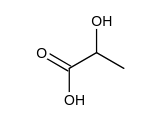
\includegraphics{smile-2d8898704cc6cc0bd550331db26da624713c28a5}\\
$\mathrm{H}_{2} \mathrm{~N}\left[\mathrm{CH}_{2}\right]_{6} \mathrm{NH}_{2}$\\
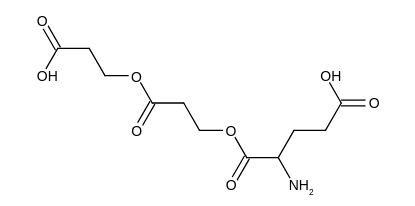
\includegraphics{smile-73e8d11180c54980c0c6a4fd46db08211bea6e00}

Nhận định nào sau đây không đúng?\\
A. Số hợp chất hữu cơ đa chức (có 2 nhóm chức giống nhau trở lên) bằng 4 .\\
B. Số hợp chất hữu cơ tạp chức (có 2 nhóm chức khác nhau trở lên) bằng 2.\\
C. Số hợp chất hữu cơ thuộc loại alcohol bằng 3 .\\
D. Số hợp chất hữu cơ thuộc loại carboxylic acid bằng 3 .

\section*{VAN DUNG}
10.15. Tại sao chỉ hai nguyên tố carbon và hydrogen nhưng tạo được nhiều hợp chất hydrocarbon?\\
10.16. Hãy giai thích:\\
a) Tại sao liên kết chủ yếu trong các hợp chất hữu cơ là liên kết cộng hoá trị?\\
b) Tại sao các phân tử hợp chất hữu cơ thường dễ nóng chảy, dễ bay hơi và it tan trong nước?\\
c) Tại sao phản ứng hữu cơ thường xảy ra theo nhiều hướng và tạo nhiều sản phẩm?\\
10.17. Sữ dụng Bảng 10.2, sách giảo khoa Hoá hoc 11, xác định và giải thích trong mỗi phổ hồng ngoại dưới đây, phổ nào tương ứng với cấu trúc của một ketone, một alcohol, một carboxylic acid, một amine bậc nhất ( $-\mathrm{NH}_{2}$ ), hay một amine bậc hai ( $-\mathrm{NH}-$ ).

\begin{figure}[h]
\begin{center}
  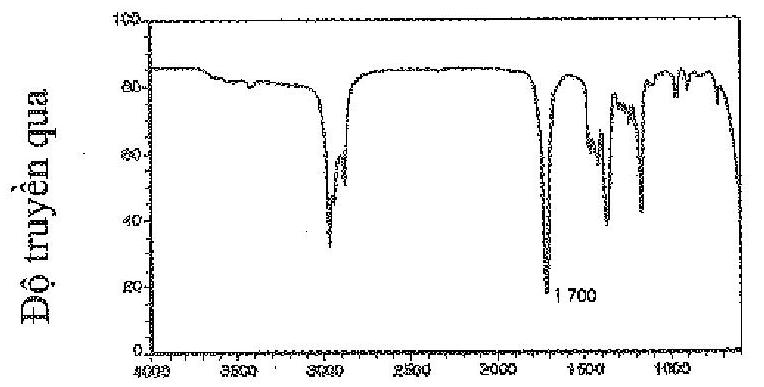
\includegraphics[width=\textwidth]{2025_10_23_fa9073eecee116ad8cf2g-38}
\captionsetup{labelformat=empty}
\caption{(a)}
\end{center}
\end{figure}

\begin{center}
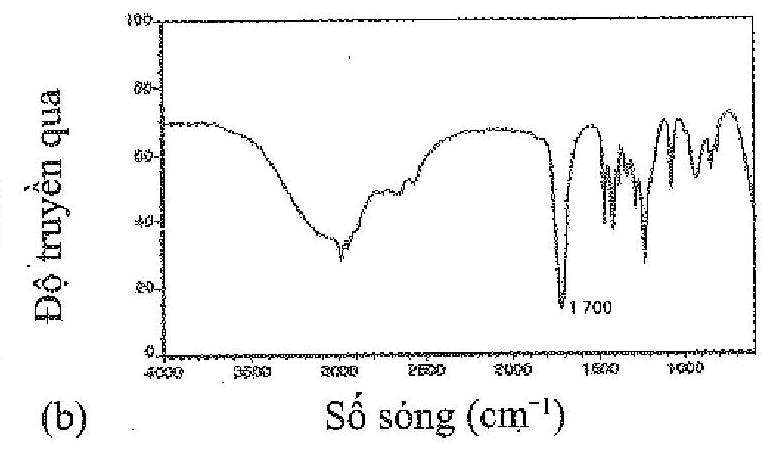
\includegraphics[max width=\textwidth]{2025_10_23_fa9073eecee116ad8cf2g-38(5)}
\end{center}

\begin{figure}[h]
\begin{center}
  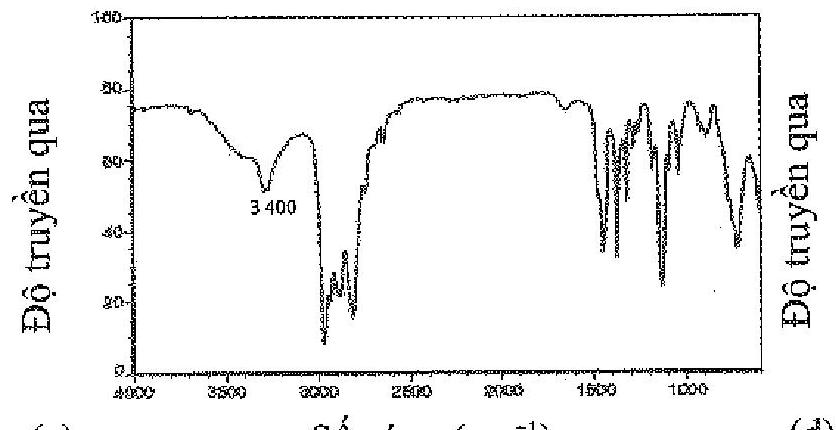
\includegraphics[width=\textwidth]{2025_10_23_fa9073eecee116ad8cf2g-38(2)}
\captionsetup{labelformat=empty}
\caption{Số sóng ( \$\textbackslash mathrm\{cm}\^{}\{-1\}\$ )\}\end{center}
\end{figure}

(c)

\begin{figure}[h]
\begin{center}
  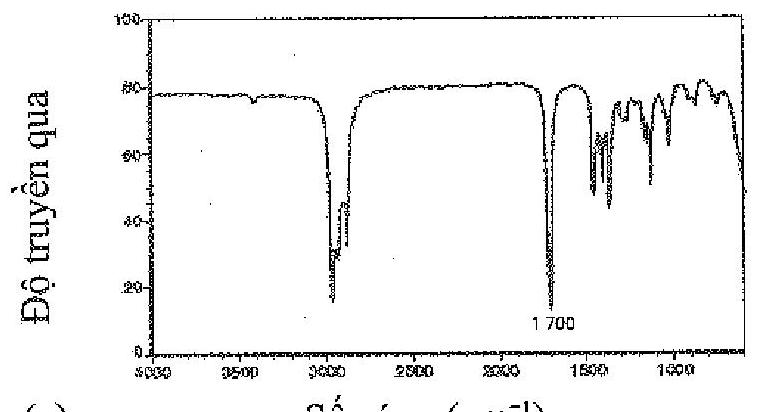
\includegraphics[width=\textwidth]{2025_10_23_fa9073eecee116ad8cf2g-38(4)}
\captionsetup{labelformat=empty}
\caption{(e)}
\end{center}
\end{figure}

\begin{figure}[h]
\begin{center}
\captionsetup{labelformat=empty}
\caption{(d)}
  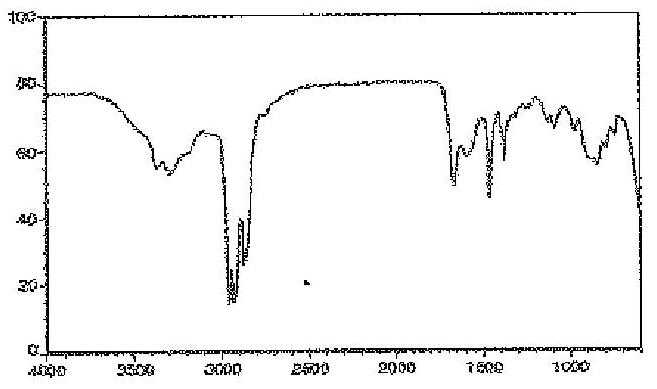
\includegraphics[width=\textwidth]{2025_10_23_fa9073eecee116ad8cf2g-38(1)}
\end{center}
\end{figure}

Số sóng ( $\mathrm{cm}^{-1}$ )

\begin{figure}[h]
\begin{center}
\captionsetup{labelformat=empty}
\caption{(d)}
  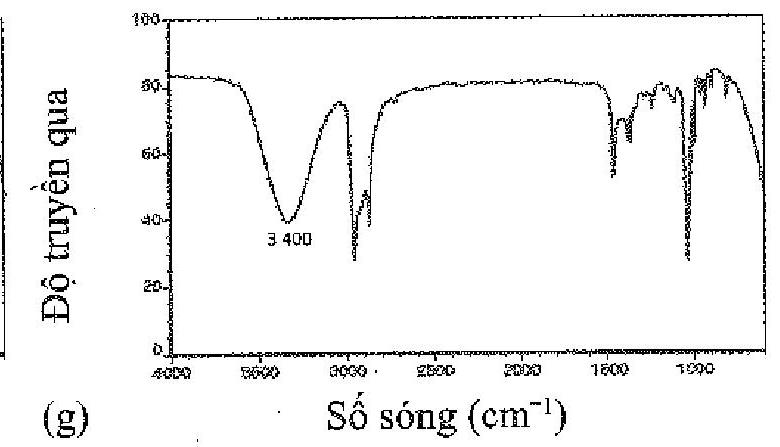
\includegraphics[width=\textwidth]{2025_10_23_fa9073eecee116ad8cf2g-38(3)}
\end{center}
\end{figure}

10.18. Chrysanthemic acid được tách từ hoa cúc, có công thức cấu tạo như sau:\\
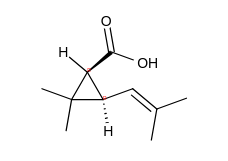
\includegraphics{smile-37b15d4293720f120e01dca31993c162972ee9a6}

chrysanthemic acid

Phồ hồng ngoai của chrysanthemic acid có năm tín hiệu sau: khoảng $1650 \mathrm{~cm}^{-1}$; khoảng $1715 \mathrm{~cm}^{-1}$, < $3000 \mathrm{~cm}^{-1}$, khoảng $3100 \mathrm{~cm}^{-1}$; khoảng $2200-3600 \mathrm{~cm}^{-1}$. Xác định các nhóm cấu trúc hình thành năm tín hiệu này.

\section*{BÀl 11}
\section*{PHUONG PHÁP TÁCH BIỆT VÀ TINH CHẾ HƠP CHÁT HƯU CO}
\section*{NHAN BIET}
11.1. Chưng cất là phương pháp tách chất dựa vào sụ khác nhau về tính chất vật lí (ở một áp suất nhất định) nào sau đây của các chất trong hỗn hợp?\\
A. Nhiệt độ sôi.\\
B. Nhiệt độ nóng chảy.\\
C. Độ tan:\\
D. Màu sắc.\\
11.2. Chiết là phương pháp dùng một dung môi thích hợp hoà tan chất cần tách chuyển sang pha lỏng (gọi là dịch chiết) và chất này được tách ra khỏi hỗn họp các chất còn lại. Tách lấy dịch chiết, giải phóng dung môi sẽ thu được\\
A. chất cần tách.\\
B. các chất còn lại.\\
C. hỗn hợp ban đầu.\\
D. họp chất khí.\\
11.3. Dung môi thích hợp được lưa chọn trong phương pháp kết tinh thường là dung môi trong đó độ tan của chất cần tinh chế\\
A. không thay đổi khi thay đồi nhiệt độ của dung địch.\\
B. tăng nhanh khi tăng nhiệt độ, tan kém ở nhiệt độ thường.\\
C. giảm nhanh khi tăng nhiệt độ, tan tốt ở nhiệt độ thường.\\
D. lớn ở nhiệt độ thường và nhỏ ở nhiệt độ cao.\\
11.4. Trong phương pháp sắc kí, hỗn hợp lỏng hoặc khí của các chất cần tách là pha động. Pha động tiếp xúc liên tục với pha tĩnh là một chất rắn có diện tích bề mặt rất lớn, có khả năng hấp phụ ... (1) ... với các chất trong hỗn hợ cần tách, khiến cho các chất trong hỗn hợp di chuyển với tốc độ ... (2)... và tách ra khỏi nhau. Cưm từ thích hợp điền vào chỗ trống (1) và (2) lần lượt là\\
A. (1) giống nhau và (2) giống nhau.\\
B. (1) khác nhau và (2) khác nhau.\\
C. (1) khác nhau và (2) giống nhau.\\
D. (1) giống nhau và (2) khác nhau.

\section*{THONC HILU}
11.5. Trong quá trình chưng cất dầu thô, người ta thu được nhiều phân đoạn dầu mỏ trong đó có xăng (thành phần chính là hỗn hợp các hydrocarbon có số nguyên tử C từ 4 đến 12 , nhiệt độ sôi khoảng từ $40^{\circ} \mathrm{C}$ đến $200^{\circ} \mathrm{C}$ ) và dầu hoả (thành phần chính là hỗn họp các hydrocarbon có số nguyên tử C từ 12 đến 16 , nhiệt độ sôi khoảng từ $200^{\circ} \mathrm{C}$ đến $250^{\circ} \mathrm{C}$ ). Sản phẩm thu được ở $150^{\circ} \mathrm{C}$ đến $200^{\circ} \mathrm{C}$ là\\
A. xăng.\\
B. dầu hoả.\\
C. xăng và dầu hoả.\\
D. dầu hoả và xăng.\\
11.6. Thêm benzene vào ống nghiệm đựng dung dịch nước bromine. Sau một thời gian quan sát thấy màu đỏ nâu của bromine\\
A. chủ yếu trong lớp nước.\\
B. chủ yếu trong lớp benzene.\\
C. phân bố đồng đều ở hai lớp.\\
D. bị mất màu hoàn toàn.\\
11.7. Xét ba yêu cầu: (a) không hoà tan tạp chất; (b) không có tương tác hoá học với chất kết tinh; (c) dễ bay hơi, dễ kiếm, rẻ tiền. Trong ba yêu cầu này, có bao nhiêu yêu cầu là cần thiết đối với dung môi được lựa chọn trong phương pháp kết tinh?\\
A. 0 .\\
B. 1.\\
C. 2.\\
D. 3 .

\section*{VAN DUNG}
11.8. Một học sinh muốn tách một hỗn hợp gồm benzoic acid, naphthalene và n-butylamine hoà tan trong ether. Đầu tiên, bạn học sinh thêm vào hỗn họp dung dịch HCl và chiết phần dung dịch nước thì thu được dung dịch A . Sau đó, bạn thêm dung dịch NaOH vào phần còn lại và chiết phần dung dịch nước thì thu được dung dịch B . Phần còn lại là dung dịch C . Xác định các chất được chuyển vào các dung dịch $\mathrm{A}, \mathrm{B}$ và C .\\
11.9. Dể tách đường saccharose (succrose, $\mathrm{C}_{12} \mathrm{H}_{22} \mathrm{O}_{11}$ ) từ nước mía (đã làm sạch tạp chất rắn và tạp chất màu), người ta dùng phương pháp kết tinh lại. Nhược điểm của việc đun nóng nước đường để bay hơi nước và kêt tinh đường là ở nhiệt độ cao, dung dịch nước đường đặc có thể bị caramel hoá (chuyển qua màu vàng nâu và có mùi đặc trưng) hoặc than hoá (chuyển thành carbon màu đen). Đề xuất biện pháp kết tinh đường tránh hiện tượng caramel hoá và than hoá này.\\
11.10. Phương pháp sắc kí giấy được áp dụng để xét nghiệm độ tinh khiết của các hoá chất trong dược khoa, phát hiện thuốc trừ sâu, thuốc diệt côn trùng trong thức ăn,... Sự tách các chất bằng phương pháp sắc kí giấy dựa chủ yếu trên sự khác nhau về sự phân bố của của các chất trên giấy (cellulose) tầm nước.\\
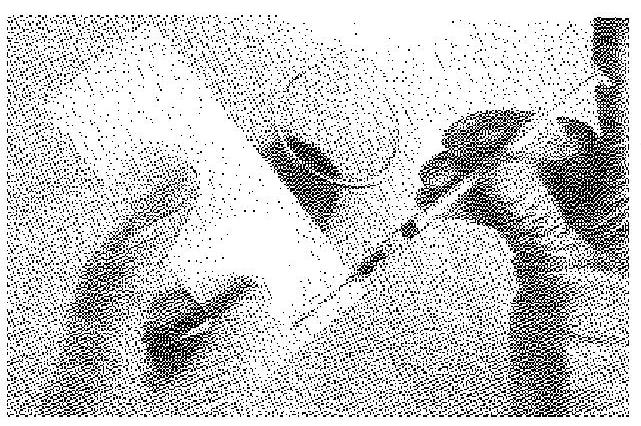
\includegraphics[max width=\textwidth, center]{2025_10_23_fa9073eecee116ad8cf2g-41}\\
Loại chất nào sẽ di chuyển nhanh và loại chất nào sẽ di chuyển chậm trên pha tĩnh là cellulose này?

\section*{BÀI 12}
\section*{CÔNG THỨC PHÂN TƯ HỘP CHẤT HƯU CO}
\section*{NHAN BILT}
12.1. Công thức phân tử cho biết thông tin nào sau đây về phân tử hợp chất hữu cơ?\\
A. Thành phần nguyên tố và số lượng nguyên tử của mỗi nguyên tố.\\
B. Thành phần nguyên tố và tỉ lệ số lượng nguyên tử của mỗi nguyên tố.\\
C. Số lượng nguyên tử mỗi nguyên tố và trật tự liên kết giữa các nguyên tử.\\
D. Tỉ lệ số lượng nguyên tử của mỗi nguyên tố và trật tự liên kết giữa các nguyên tữ.\\
12.2. Công thức nào sau đây là công thức phân tử của acetic acid?\\
A. $\mathrm{CH}_{3}-\mathrm{COOH}$.\\
B. $\mathrm{C}_{2} \mathrm{H}_{4} \mathrm{O}_{2}$.\\
C. $\mathrm{CH}_{2} \mathrm{O}$.\\
D. $\mathrm{C}_{\mathrm{x}} \mathrm{H}_{\mathrm{y}} \mathrm{O}_{z}$.\\
12.3. Công thức phân tử của methyl formate và glucose lần lượt là $\mathrm{C}_{2} \mathrm{H}_{4} \mathrm{O}_{2}$ và $\mathrm{C}_{6} \mathrm{H}_{12} \mathrm{O}_{6}$. Công thúc đon giản nhất của hai chất này là\\
A. $\mathrm{CH}_{2} \mathrm{O}$.\\
B. $\mathrm{C}_{2} \mathrm{H}_{4} \mathrm{O}_{2}$.\\
C. $\mathrm{C}_{4} \mathrm{H}_{8} \mathrm{O}_{4}$.\\
D. $\mathrm{C}_{6} \mathrm{H}_{12} \mathrm{O}_{6}$.\\
12.4. Trong phương pháp phổ khối lương, đối với các họp chát đơn giản, thường mảnh có giá trị $\mathrm{m} / \mathrm{z}$ lớn nhất ứng với mảnh ion phân tư $\left[\mathrm{M}^{+}\right]$và giá trị này bằng giá trị $\_\_\_\_$ của chất nghiên cứu. Cụm từ thích họp điền vào chỗ trống là.\\
A. phân tử khối.\\
B. nguyên tữ khối.\\
C. điện tích ion.\\
D. khối lượng.

\section*{THONG MILU}
12.5. Hình sau đây là phổ khối lượng của phân tử acetic acid.\\
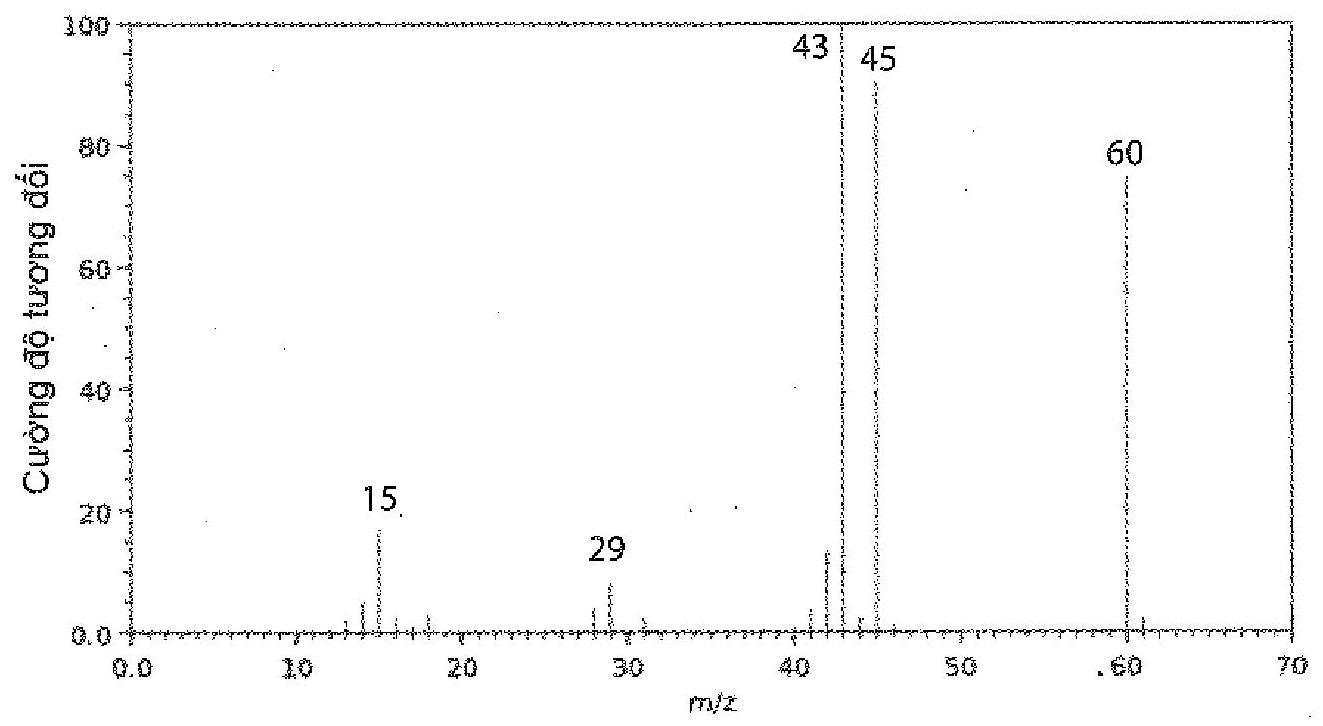
\includegraphics[max width=\textwidth, center]{2025_10_23_fa9073eecee116ad8cf2g-42(1)}

Phân tử khối của acetic acid bằng\\
A. 43 .\\
B. 45 .\\
C. 60 .\\
D. 29 .\\
12.6. Hình sau đây là phổ khối lượng của phân tử benzene.\\
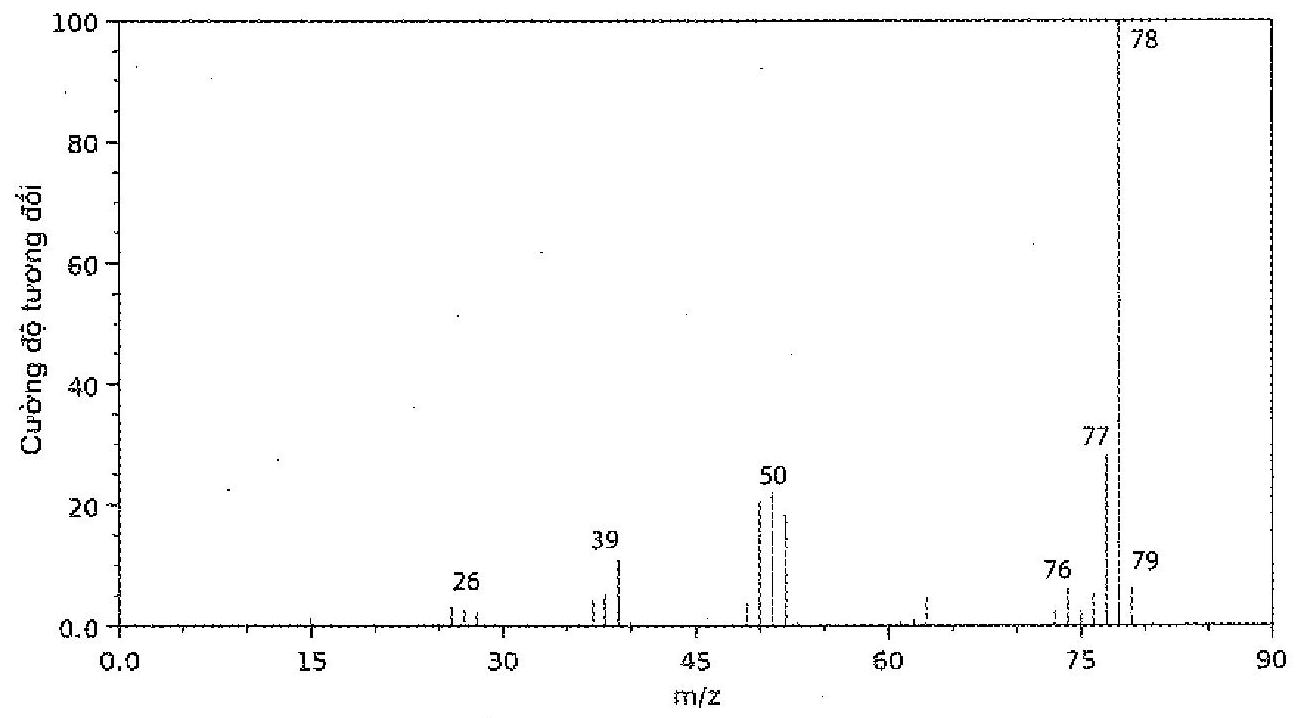
\includegraphics[max width=\textwidth, center]{2025_10_23_fa9073eecee116ad8cf2g-42}

Phân tử khối của benzene bằng\\
A. 76 .\\
B. 77.\\
C. 78.\\
D. 79 .\\
12.7. Một họp chất hữu cơ A chưa $32 \% \mathrm{C}, 4 \% \mathrm{H}$ và $64 \% . \mathrm{O}$ về khối lượng. Biết một phân tữ A có 6 nguyên tữ oxygen, công thức phân tữ của A là\\
A. $\mathrm{C}_{2} \mathrm{H}_{3} \mathrm{O}_{3}$.\\
B. $\mathrm{C}_{4} \mathrm{H}_{6} \mathrm{O}_{6}$.\\
C. $\mathrm{C}_{6} \mathrm{H}_{12} \mathrm{O}_{6}$.\\
D. $\mathrm{C}_{6} \mathrm{H}_{4} \mathrm{O}_{6}$.

\section*{VAN DUNG}
12.8. Một hợp chất hữu co X chứa $37,5 \% \mathrm{C}, 3,2 \% \mathrm{H}$ và $59,3 \% \mathrm{~F}$ về khối lượng. Cho bay hơi $1,00 \mathrm{~g}$ chất này tại $90^{\circ} \mathrm{C}$ với áp suât 0,50 bar thì thể tích thu được là $0,93 \mathrm{~L}$. Xác định công thức phân tử của X .\\
12.9. Vitamin C (ascorbic acid) chứa $40,92 \% \mathrm{C}, 4,58 \% \mathrm{H}$ và $54,50 \% \mathrm{O}$ về khối lượng. Hình sau đây là phổ khối lượng của ascorbic acid:\\
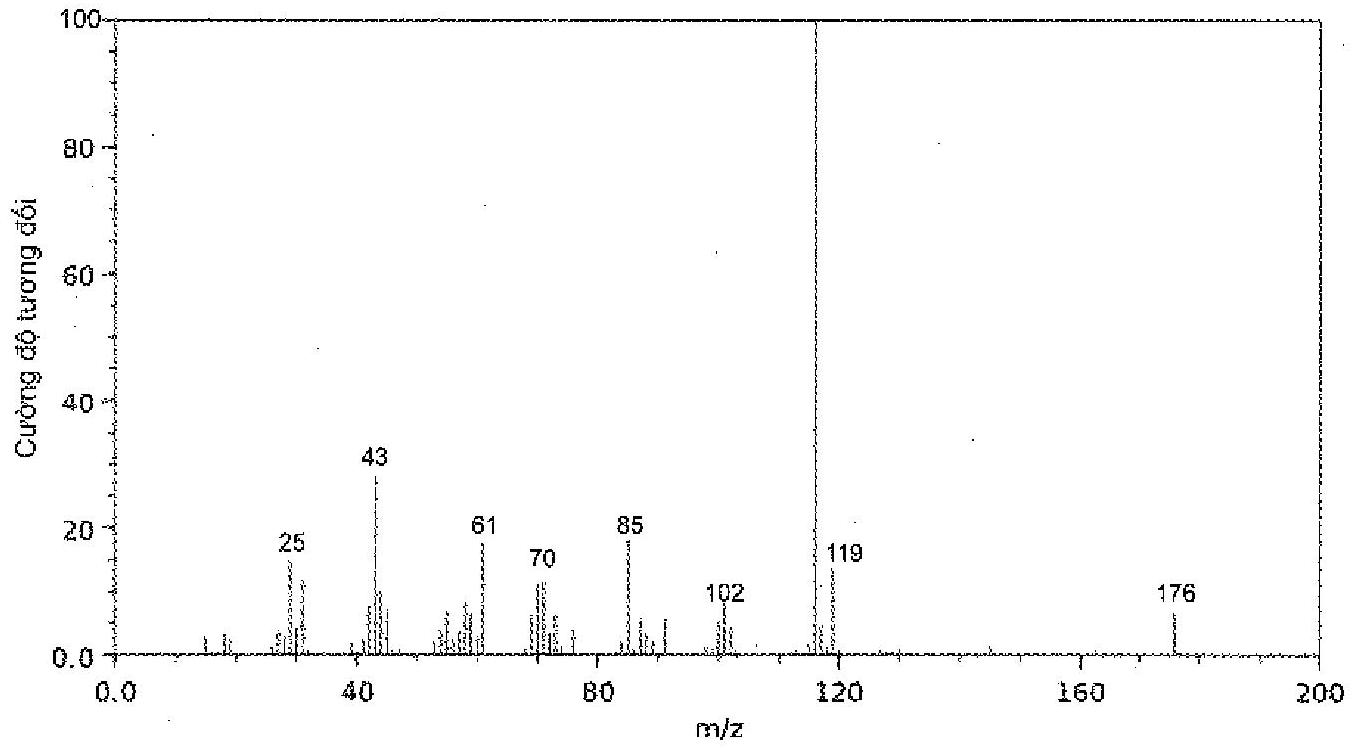
\includegraphics[max width=\textwidth, center]{2025_10_23_fa9073eecee116ad8cf2g-43}

Xác định công thức thực nghiệm và công thức phân tử của ascorbic acid.\\
12.10. Đốt cháy $20,63 \mathrm{mg}$ hợp chất Y , chỉ chứa $\mathrm{C}, \mathrm{H}$, và O , bằng lượng dư khí oxygen tão $57,94 \mathrm{mg} \mathrm{CO}_{2}$ và $11,85 \mathrm{mg} \mathrm{H}_{2} \mathrm{O}$.\\
a) Tính khối lượng (theo mg ) của $\mathrm{C}, \mathrm{H}$ và O trong hợp chất Y .\\
b) Xác định công thức thực nghiệm của Y.\\
c) Dựa trên phổ knối lượng của Y như hình cho dưới đây, xác định công thức phân tữ của Y.\\
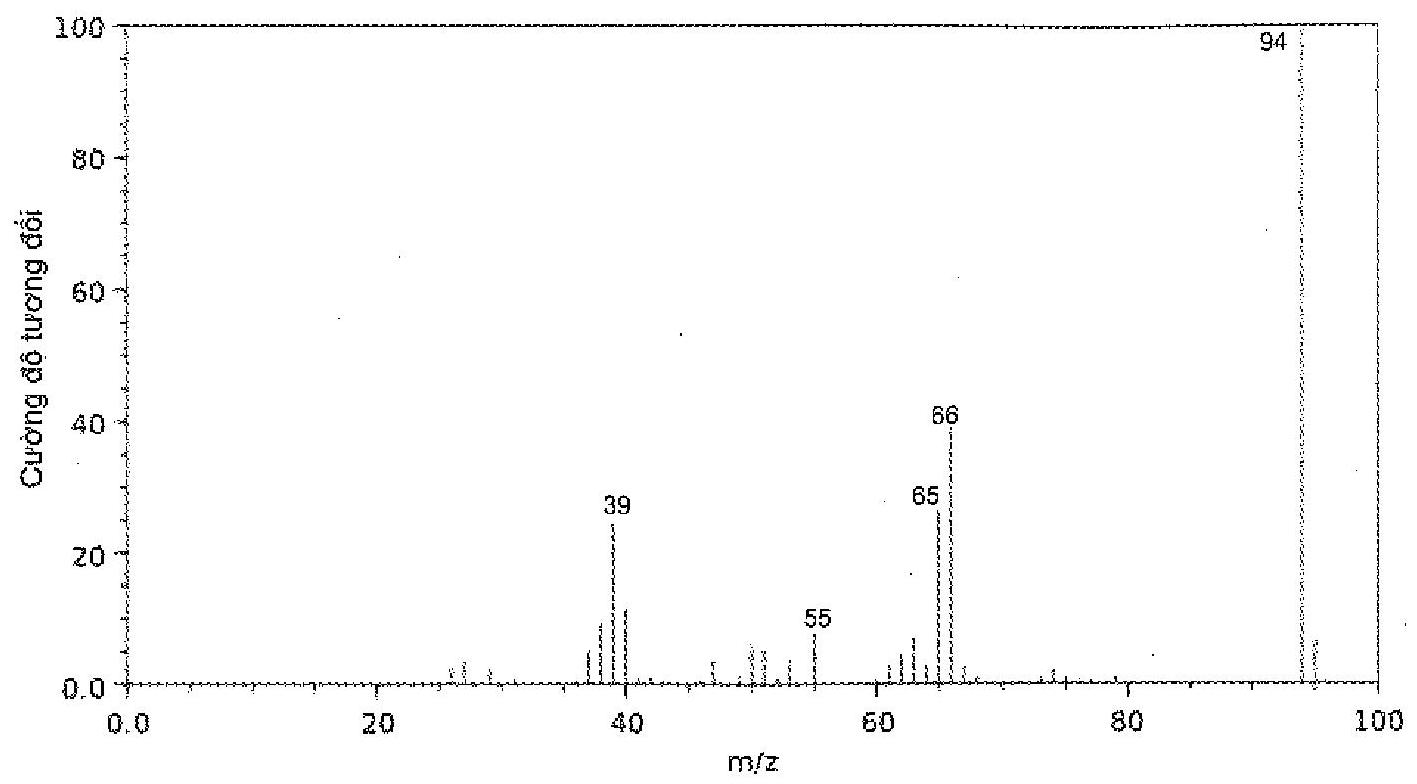
\includegraphics[max width=\textwidth, center]{2025_10_23_fa9073eecee116ad8cf2g-44}

\section*{BÀl 13}
\section*{CẤU TẠO HOÁ HỌC HỢ CHÁT HỮU CƠ}
\section*{NHAN BIET}
13.1. Cấu tạo hoá học là ..... giữa các nguyên tử trong phân tử. Cụm từ thích hợp điền vào chỗ trống là\\
A. thứ tự liên kết.\\
B. phản úng.\\
C. liên kết.\\
D. tỉ lệ số lượng.\\
13.2. Có 4 loại cấu tạo mạch phân tử: (a) mạch hở không phân nhánh; (b) mạch hở phân nhánh; (c) mạch vòng không phân nhánh và (d) mạch vòng phân nhánh. Trong phân tử hợp chất hữu co, các nguyên tử carbon có thể liên kết với chính nó hình thành bao nhiêu loại mạch?\\
A. 1 .\\
B. 2 .\\
C. 3 .\\
D. 4 .\\
13.3. Trong các yếu tố: (a) thành phần nguyên tố; (b) số lượg nguyên tử mỗi nguyên tố và (c) thứ tự liên kết của các nguyên tử trong phân tử, thì tính chất của phân tử họp chất hữu cơ phụ thuộc vào các yếu tố\\
A. (a) và (b).\\
B. (b) và (c).\\
C. (a) và (c).\\
D. (a), (b) và (c).\\
13.4. Những hợp chất hữu cơ khác nhau nhưng có cùng công thức phân tữ được goi là các chất\\
A. đồng phân của nhau.\\
B. đồng đẳng của nhau.\\
C. đồng vị của nhau.\\
D. đồng khối của nhau.\\
13.5. Các chất hữu cơ có tính chất hoá học tương tự nhau và thành phần phân tử hơn kém nhau một hay nhiều nhóm $\mathrm{CH}_{2}$ được gọi là các chất\\
A. đồng phân của nhau.\\
B. đồng đẳng của nhau.\\
C. đồng vị của nhau.\\
D. đồng khối của nhau.

\section*{THONG HILU}
13.6. Công thức nào dưới đây là công thức cấu tạo?\\
A. $\mathrm{HOCH}_{2} \mathrm{CH}_{2} \mathrm{OH}$.\\
B. $\mathrm{C}_{2} \mathrm{H}_{6} \mathrm{O}_{2}$.\\
C. $\mathrm{CH}_{3} \mathrm{O}$.\\
D. $\mathrm{C}_{n} \mathrm{H}_{3 n} \mathrm{O}_{n}$.\\
13.7. Cặp chất nào dưới đây là đồng đẳng của nhau?\\
A. $\mathrm{CH}_{3} \mathrm{CH}=\mathrm{CH}_{2}$ và $\mathrm{CH}_{3}-\mathrm{CH}_{2}-\mathrm{CH}_{2}-\mathrm{CH}_{3}$.\\
B. $\mathrm{CH}_{2}=\mathrm{CH}-\mathrm{CH}=\mathrm{CH}_{2}$ và $\mathrm{CH}_{3} \mathrm{C} \equiv \mathrm{CH}$.\\
C. $\mathrm{CH}_{3} \mathrm{CH}_{2} \mathrm{CH}_{2} \mathrm{CH}_{3}$ và $\left(\mathrm{CH}_{3}\right)_{2} \mathrm{CHCH}_{3}$.\\
D. $\mathrm{CH}_{2}=\mathrm{CH}-\mathrm{CH}=\mathrm{CH}_{2}$ và $\mathrm{CH}_{2}=\mathrm{C}\left(\mathrm{CH}_{3}\right)-\mathrm{CH}=\mathrm{CH}_{2}$.\\
13.8. Cạp chất nào dưới đây là đồng đẳng của nhau?\\
A. $\mathrm{CH}_{3} \mathrm{OH}$ và $\mathrm{CH}_{3} \mathrm{CH}_{2} \mathrm{CH}_{2} \mathrm{CH}_{2} \mathrm{OH}$.\\
B. $\mathrm{CH}_{3} \mathrm{CH}_{2} \mathrm{OH}$ và $\mathrm{HOCH}_{2} \mathrm{CH}_{2} \mathrm{OH}$.\\
C. $\mathrm{CH}_{3} \mathrm{CH}_{2} \mathrm{CHO}$ và $\mathrm{CH}_{3} \mathrm{COCH}_{2} \mathrm{CH}_{3}$.\\
D. $\mathrm{CH}_{3} \mathrm{COOH}$ và $\mathrm{CH}_{3} \mathrm{COOCH}_{3}$.\\
13.9. Cặp chất nào dưới đây là đồng phân loại nhóm chức?\\
A. $\mathrm{CH}_{3} \mathrm{OCH}_{3}$ và $\mathrm{CH}_{3} \mathrm{CH}_{2} \mathrm{CH}_{2} \mathrm{OH}$.\\
B. $\mathrm{CH}_{3} \mathrm{COOH}$ và $\mathrm{HCOOCH}_{3}$.\\
C. $\mathrm{CH}_{2}=\mathrm{CH}-\mathrm{CH}_{3}$ và $\mathrm{CH}_{2}=\mathrm{C}\left(\mathrm{CH}_{3}\right) \mathrm{CH}_{3}$.\\
D. $\mathrm{CH}_{3} \mathrm{CH}_{2} \mathrm{CH}_{2} \mathrm{OH}$ và $\mathrm{CH}_{3} \mathrm{CH}(\mathrm{OH}) \mathrm{CH}_{3}$.\\
13.10. Cặp chất nào dưới đây là đồng phân vị trí nhóm chức?\\
A. $\mathrm{CH}_{3} \mathrm{OCH}_{2} \mathrm{CH}_{3}$ và $\mathrm{CH}_{3} \mathrm{CH}_{2} \mathrm{CH}_{2} \mathrm{OH}$.\\
B. $\mathrm{CH}_{3} \mathrm{COCH}_{3}$ và $\mathrm{CH}_{3} \mathrm{CH}_{2} \mathrm{CH}=\mathrm{O}$.\\
C. $\mathrm{CH} \equiv \mathrm{CCH}_{2} \mathrm{CH}_{3}$ và $\mathrm{CH}_{3} \mathrm{CH}_{2}=\mathrm{CH}-\mathrm{CH}=\mathrm{CH}_{2} \mathrm{CH}_{3}$.\\
D. $\mathrm{CH}_{3} \mathrm{CH}_{2} \mathrm{CH}_{2} \mathrm{OH}$ và $\mathrm{CH}_{3} \mathrm{CH}(\mathrm{OH}) \mathrm{CH}_{3}$.

\section*{VAN DUNG}
13.11. Xác định loại đồng phân cấu tạo có thể có và viết các đồng phân cấu tạo có thể có của các hợp chất có công thức phân tử $\mathrm{C}_{5} \mathrm{H}_{12}$ và $\mathrm{C}_{4} \mathrm{H}_{8}$.\\
13.12. Xác định loại đồng phân cấu tạo có thể có và viết các đồng phân cấu tạo có thể có của các hợp chất có công thức phân tử $\mathrm{C}_{4} \mathrm{H}_{10} \mathrm{O}$.

\section*{BÀ 14}
\section*{ÔN TÂP CHƯONG 3}
\section*{NHAN BICT}
14.1. Cho các phát biểu sau:\\
(1) Phân tử hợp chất hữu cơ nhất thiết phải chứa carbon;\\
(2) Liên kết chủ yếu trong phân tự hợp chất hữu cơ là liên kết ion;\\
(3) Hợp chất hữu cơ thường khó nóng chảy và khó bay hơi;\\
(4) Họp chất hữu cơ thường không tan hoặc ít tan trong nước;\\
(5) Phản ứng của các hợp chất hữu cơ thường chậm, không hoàn toàn, không theo một hướng nhất định;\\
(6) Các hợp chất hữu cơ thường khó cháy và khó bị phân huỷ dưới tác dụng của nhiệt. Số phát biểu đúng là\\
A. 3 .\\
B. 4\\
C. 5.\\
D. 6 .\\
14.2. Cho hợ chất hữu cơ $X$ có công thức cấu tạo sau:\\
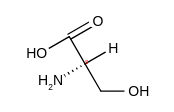
\includegraphics{smile-b0e6b84729e003375d09c255ac60ff7eaf53bd73}

$L$-serine

X không chúa loại nhóm chức nào sau đây?\\
A. Alcohol.\\
B. Aldehyde.\\
C. Amine.\\
D. Carboxyl.\\
14.3. Cho các hợp chất hữu cơ sau:\\
(1) $\mathrm{CH}_{4}$;\\
(2) $\mathrm{CH}_{3} \mathrm{OH}_{3}$\\
(3) $\mathrm{CH}_{2}=\mathrm{CH}_{2}$;\\
(4) $\mathrm{CH}_{2} \mathrm{OH}-\mathrm{CHOH}-\mathrm{CH}_{2} \mathrm{OH}$;\\
(5) $\mathrm{CH} \equiv \mathrm{CH}$;\\
(6) $\mathrm{CH}_{3} \mathrm{CH}=\mathrm{O}$;\\
(7) $\mathrm{CH}_{3} \mathrm{COOH}$;\\
(8) $\mathrm{HOOC}\left[\mathrm{CH}_{2}\right]_{4} \mathrm{COOH}$;\\
(9) $\mathrm{C}_{6} \mathrm{H}_{6}$ (benzen); (\\
(10) $\mathrm{H}_{2} \mathrm{NCH}_{2} \mathrm{COOH}$; (11) $\mathrm{CH}_{2} \mathrm{OH}[\mathrm{CHOH}]_{4} \mathrm{CH}=\mathrm{O}$.

Nhận định nào sau đây không đúng?\\
A. Có hai hợp chât hữu cơ đa chức và hai hợp chất hữu co tạp chức.\\
B. Có hai họp chât thuộc loại alcohol và ba hợp chất thuộc loại carboxylic acid.\\
C. Có bốn họp chất thuộc loại hydrocarbon, trong đó có hai hydrocarbon không no.\\
D. Có bảy họp chất thuộc loại dẫn xuất của hydrocarbon, trong đó ba hợp chất don chúc.\\
14.4. Cho các phát biểu sau:\\
(1) Cấu tạo hoá học là trật tự liên kết giữa các nguyên tử trong phân tử;\\
(2) Cấu tạo hoá học khác nhau tạo ra các chất khác nhau;\\
(3) Trong phân tử họp chất hữu co, nguyên tử carbon luôn có hoá trị bốn;\\
(4) Trong phân tử hợp chất hữu co, các nguyên tử carbon chỉ liên kết với nguyên tử của nguyên tố khác.\\
(5) Tính chất vật lí và tính chất hoá học của hợp chất hữu cơ phụ thuộc vào thành phần phân tử và cấu tạo hoá học.\\
Số phát biểu đúng là\\
A. 2 .\\
B. 3 .\\
C. 4 .\\
D. 5 .\\
14.5. Cho các phát biểu sau:\\
(1) Công thức cấu tạo biểu diễn kiểu liên kết và trật tự liên kết giữa các nguyên tữ trong phân tứ;\\
(2) Chất đồng phân có cùng công thức phân tữ nhưng có thể khác nhau vè loại nhóm chửc, mạch carbon, vị trí liên kết pi ( $\pi$ ) hoặc vị trí nhóm chức;\\
(3) Chất đồng đẳng có cấu tạo và tính chất tương tự, nhưng thành phần phân tử khác nhau một hay nhiều nhóm $\mathrm{CH}_{2}$.\\
Số phát biểu đúng là\\
A. 0 .\\
B. 1 .\\
C. 2 .\\
D. 3 .

\section*{THONG HILO}
14.6. Nhận định nào sau đây không đúng?\\
A. Người ta có thể chiết tách các chất hữu cơ hữu ich từ thuốc Bắc bằng cách ngâm thuốc Bắc trong dung dịch ethanol.\\
B. Sau khi ép cây mía và làm sạch các chất bẩn rắn cũng như chất bẩn màu, người ta thu được dung dịch nước đường. Cô cạn nước đường ở áp suất thấp sẽ tách được đường.\\
C. Sau khi chưng cất cây sả bằng hơi nước, người ta thu được lớp tinh dầu (chứa terpene) nổi trên mặt nước. Dùng phương pháp chiết sẽ tách riêng được lớp tinh dầu.\\
D. Để tách ethanol (ethylic alcohol) từ hỗn hợp với nước và bã rượu. Dùng kĩ thuật lọc tách sẽ tách riêng được ethanol ra khỏi hỗn hợp này.\\
14.7. Cho các cặp chất sau: (a) $\mathrm{CH}=\mathrm{CH}$ và $\mathrm{CH}_{2}=\mathrm{C}=\mathrm{CH}_{2}$; (b) $\mathrm{CH} \equiv \mathrm{CH}^{2}$ và $\mathrm{CH}_{3} \mathrm{CH}_{2} \mathrm{C} \equiv \mathrm{CH}$; (c) $\mathrm{CH}_{3} \mathrm{CH}_{2} \mathrm{OH}$ và $\left(\mathrm{CH}_{3}\right)_{2} \mathrm{CHCH}_{2} \mathrm{OH}$; (d) $\mathrm{C}_{6} \mathrm{H}_{5} \mathrm{OH}$ và $\mathrm{C}_{6} \mathrm{H}_{4}(\mathrm{OH})_{2}$; (e) $\mathrm{HCH}=\mathrm{O}$ và $\mathrm{CH}_{3} \mathrm{COCH}_{3}$.\\
Số cặp chất là đồng đẳng của nhau là\\
A. 1 .\\
B. 2 .\\
C. 3 .\\
D. 4 .\\
14.8. Cho các cặp chất sau: (a) $\mathrm{CH} \equiv \mathrm{CH}$ và $\mathrm{CH}_{3}-\mathrm{C} \equiv \mathrm{CH}$; (b) $\left(\mathrm{CH}_{3}\right)_{2} \mathrm{C}=\mathrm{CH}_{2}$ và $\mathrm{CH}_{3} \mathrm{CH}_{2} \mathrm{CH}=\mathrm{CH}_{2}$; (c) $\mathrm{CH}_{3} \mathrm{CH}_{2} \mathrm{CH}=\mathrm{O}$ và $\mathrm{CH}_{3} \mathrm{COCH}_{3}$; (d) $\mathrm{CH}_{3} \mathrm{CH}_{2} \mathrm{CH}_{2} \mathrm{OH}$ và $\mathrm{CH}_{3} \mathrm{CH}(\mathrm{OH}) \mathrm{CH}_{3}$; (e) $\mathrm{CH}_{2}=\mathrm{CH}-\mathrm{CH}_{2}-\mathrm{CH}_{3}$ và $\mathrm{CH}_{2}=\mathrm{CH}-\mathrm{CH}=\mathrm{CH}_{2}$.\\
Số cặp chất là đồng phân của nhau là\\
A. 1 .\\
B. 2 .\\
C. 3 .\\
D. 4 .\\
14.9. Các hợp chất sau đây thuộc loại hydrocarbon nào?\\
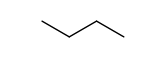
\includegraphics{smile-c8d5b196e3330e32fc4032c3f1e3494df534800e}

butane\\
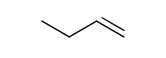
\includegraphics{smile-484155c357519701b1ad5e4d7f9341e194acd2a4}

but-1-ene

\begin{figure}[h]
\begin{center}
  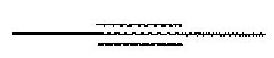
\includegraphics[width=\textwidth]{2025_10_23_fa9073eecee116ad8cf2g-49}
\captionsetup{labelformat=empty}
\caption{but-2-yne}
\end{center}
\end{figure}

14.10. Phân tích định lượng Atabrine, một loại thuốc chống sốt rét, người ta xác định được chất này chưa 69,1\% carbon, 7,5\% hydrogen, 10,5\% nitrogen, 8,9\% chlorine và $4,0 \%$ oxygen về khối lượng. Hãy xác định công thức thực nghiệm của Atabrine.

\section*{YAN DUNG}
14.11. Một mẫu aspirin được xác định là có chứa $60,00 \%$ carbon, $4,44 \%$ hydrogen và $35,56 \%$ oxygen về khối lượng. Phổ khối lượng của aspirin như hình sau đây. Xác định công thức phân tử của Aspirin.\\
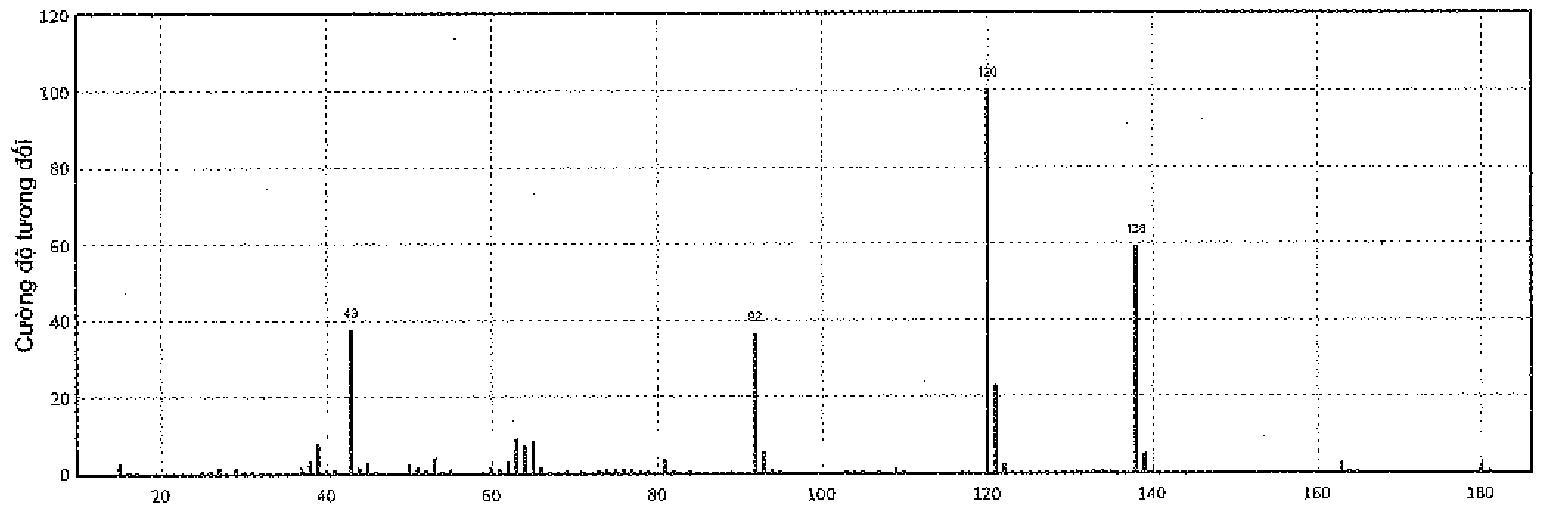
\includegraphics[max width=\textwidth, center]{2025_10_23_fa9073eecee116ad8cf2g-49(1)}\\
14.12. Xác định loại đồng phân cấu tạo có thể có và viết các đồng phân cấu tạo có thể có của các hợp chất có công thức phân tử $\mathrm{C}_{4} \mathrm{H}_{9} \mathrm{Cl}$ và $\mathrm{C}_{8} \mathrm{H}_{10}$ (hydrocarbon thom).

\section*{Churong 4 HYDROCARBON}
\section*{BÀI 15}
\section*{ALKANE}
\section*{MHAN BIET}
15.1. Công thức phân tử nào sau đây không phải là công thức của một alkane?\\
A. $\mathrm{C}_{2} \mathrm{H}_{6}$.\\
B. $\mathrm{C}_{3} \mathrm{H}_{6}$.\\
C. $\mathrm{C}_{4} \mathrm{H}_{10}$,\\
D. $\mathrm{C}_{5} \mathrm{H}_{12}$.\\
15.2. Pentane là tên theo danh pháp thay thế của\\
A. $\mathrm{CH}_{3}\left[\mathrm{CH}_{2}\right]_{2} \mathrm{CH}_{3}$.\\
B. $\mathrm{CH}_{3}\left[\mathrm{CH}_{2}\right]_{3} \mathrm{CH}_{3}$,\\
C. $\mathrm{CH}_{3}\left[\mathrm{CH}_{2}\right]_{4} \mathrm{CH}_{3}$.\\
D. $\mathrm{CH}_{3}\left[\mathrm{CH}_{2}\right]_{5} \mathrm{CH}_{3}$.\\
15.3. $\left(\mathrm{CH}_{3}\right)_{2} \mathrm{CH}-\mathrm{CH}_{3}$ có tên theo danh pháp thay thế là\\
A. 2-methylpropane.\\
B. isobutan.\\
B. butane.\\
D. 2-methylbutane.\\
15.4. Phát biểu nào sau đây không đúng?\\
A. Trong phân tử alkane chỉ chứa các liên kết $\sigma$ bền vững.\\
B. Các phân tữ alkane hầu như không phân cực.\\
C. Ở điều kiện thường các alkane tương đối trơ về mặt hoá học.\\
D. Trong phân tử methane, bốn liên kết $\mathrm{C}-\mathrm{H}$ hướng về bốn đỉnh của một hình vuông.\\
15.5. Phát biểu nào sau đây không đúng (ở điều kiện thường)?\\
A. Các alkane từ Cl đến C 4 và neopentane ở trạng thái khí.\\
B. Các alkane từ C5 đến C17 (trừ neopentane) ở trạng thái lỏng.\\
C. Các alkane không tan hoặc tan rât it trong nước và nhẹ hơn nước.\\
D. Các alkane không tan hoặc tan rât ít trong các dung môi hữu co.\\
15.6. Nhận xét nào sau đây là đúng về tính chất hoá học của ankan?\\
A. Khá trơ về mặt hoá học, phản ứng đặc trưng là thế và tách,\\
B. Hoạt động hoá học mạnh, phản ưng đặc trưng là thế và tách.\\
C. Khá trơ về mặt hoá học, phản úng đặc trưng là cộng và trùng hợp.\\
D. Hoạt động hoá học mạnh, phản ứng đặc trưng là cộng và trùng hợp.\\
15.7. Cho các chất sau: chloromethane, dichloromethane, trichloromethane và tetrachloromethane.\\
Số chất là sản phẩm của phản ứng xảy ra khi trộn methane với chlorine và chiếu ánh sáng tữ ngoại là\\
A. 1 .\\
B. 2 .\\
C. 3 .\\
D. 4 .\\
15.8. Cho các chất sau: $(\mathrm{X})$ 1-chloropropane và $(\mathrm{Y})$ 2-chloropropane. Sản phẩm của phản ứng monochlorine hoá propane là\\
A. $(\mathrm{X})$.\\
B. (Y).\\
C. cả hai chất.\\
D. chất khác $\mathrm{X}, \mathrm{Y}$.\\
15.9. Cracking alkane là quá trình phân cắt liên kết $\mathrm{C}-\mathrm{C}$ (bẻ gãy mạch carbon) của các alkane mạch dài để tạo thành hỗn hợp các hydrocarbon có mạch carbon\\
A. ngẳn hơn.\\
B. dài hon.\\
C. không đổi.\\
D. thay đôi.\\
15.10. Phát biểu nào sau đây không đúng về phản ứng reforming alkane?\\
A. Chuyển alkane mạch không phân nhánh thành các alkane mạch phân nhánh.\\
B. Chuyển alkane mạch không phân nhánh thành các hydrocarbon mạch vòng.\\
C. Số nguyên tử carbon của chất tham gia và của sản phẩm bằng nhau.\\
D. Nhiệt độ sôi của sản phẩm lớn hơn nhiều so với alkane tham gia phản ứng.\\
15.11. Phát biểu nào sau đây về ứng dụng của alkane không đúng?\\
A. Propane $\mathrm{C}_{3} \mathrm{H}_{8}$ và butane $\mathrm{C}_{4} \mathrm{H}_{10}$ đượe sử dụng làm khí đốt.\\
B. Các alkane $\mathrm{C} 6, \mathrm{C} 7, \mathrm{C} 8$ là nguyên liệu để sản xuất một số hydrocarbon thơm.\\
C. Các alkane lỏng được sử đụng làm nhiên liệu như xăng hay dầu diesel.\\
D. Các alkane từ C11 đến C20 được dùng làm nến và sáp.

\section*{THONG HIEU}
15.12. Alkane X có công thức phân tữ $\mathrm{C}_{6} \mathrm{H}_{14}$. Số công thức cấu tạo của X là\\
A. 2 .\\
B. 3 .\\
C. 4 .\\
D. 5 .\\
15.13. Alkane $\left(\mathrm{CH}_{3}\right)_{3} \mathrm{C}-\mathrm{CH}_{2}-\mathrm{CH}\left(\mathrm{CH}_{3}\right)_{2}$ có tên gọi là\\
A. 2,2,4-trimethylpentane.\\
B. $2,4,4$-trimethylpentane.\\
C. pentamethylpropane.\\
D. trimetylpentane.\\
15.14. Tên goi của alkane nào sau đây đúng?\\
A. 2-ethylbutane.\\
B. 2,2-dimethylbutane.\\
C. 3-methylbutane.\\
D. 2,3,3-trimethylbutane.\\
15.15. Cho các alkane kèm theo nhiệt độ nóng chảy và nhiệt độ sôi $\left({ }^{\circ} \mathrm{C}\right)$ sau: propane ( $-187,7$ và $-42,1$ ), butane ( $-138,3$ và $-0,5$ ), pentane ( $-129,7$ và 36,1 ), hexane ( $-95,3$ và 68,7 ).\\
Số alkane tồn tại ở thể khí ở điều kiện thường là\\
A. 1 .\\
B. 2 .\\
C. 3 .\\
D. 4 .\\
15. 16. Trộn neopentane với chlorine và chiếu ánh sáng tử ngoại thì thu đượ tối đa bao nhiêu sản phẩm monochlorine?\\
A. 1 .\\
B. 2 .\\
C. 3 .\\
D. 4 .\\
15.17. Cho các chất sau: (1) 2-methylbutane; (2) 2-methylpentane; (3) 3-methylpentane; (4) 2,2-dimethylbutane và (5) benzene.

Trong số các chất này, có bao nhiêu chất có thể là sản phẩm reforming hexane ?\\
A. 5 .\\
B. 2 .\\
C. 3 .\\
D. 4 .\\
15.18. Oxi hoá butane bằng oxygen ở $180^{\circ} \mathrm{C}$ và 70 bar tạo thành sản phẩm hữu co X duy nhất. X là\\
A. HCOOH .\\
B. $\mathrm{CH}_{3} \mathrm{COOH}$.\\
C. $\mathrm{C}_{2} \mathrm{H}_{5} \mathrm{COOH}$.\\
D. $\mathrm{CO}_{2}$.

\section*{VARI DUNG}
15.19. (a) Viết công thức cấu tạo của các alkane có tên gọi sau:

Pentane; 2-methylbutane (isopentane) và 2,2-dimethylpropane (neopentane).\\
(b) Gọi tên các alkane sau:

(i)\\
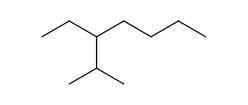
\includegraphics{smile-07f6b3b30c07a4b191c70636720818c1c00be6ec}

(ii)\\
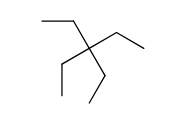
\includegraphics{smile-5c3ef0b26c358d213a353df4c838df9ace79b711}\\
15.20. Cho các alkane sau: (a) butane; (b) isobutane (2-methylpropane) và (c) neopentan (2,2-dimethylpropane).\\
Số dẫn xuất một lần thế được tạo thành khi chlorine hoá các hydrocarbon trên là bao nhiêu? Viết công thức cấu tạo và gọi tên các sản phẩm.\\
15.21. Monochlorine hoá propane (có chiếu sáng, ở $25^{\circ} \mathrm{C}$ ), thu được $45 \%$ 1-chloropropane và 55\% 2-chloropropane; còn monobromine hoá propane (có chiếu sáng và đun nóng đến $127^{\circ} \mathrm{C}$ ), thu được $4 \%$ 1-bromopropane và $96 \%$ 2-bromopropane. Dựa trên các kết quả thực nghiệm này, hãy nhận xét về:\\
(a) quan hệ giữa khả năng tham gia phản ứng thế của alkane và bậc của carbon;\\
(b) khả năng phản ứng của các halogen và tính chọn lọc vị trí thế của các halogen.\\
15.22. Tính nhiệt hình thành chuẩn của methane và propane. Biết nhiệt cháy chuẩn của methane và propane lần lượt bằng $-890 \mathrm{~kJ} / \mathrm{mol}$ và $-2216 \mathrm{~kJ} / \mathrm{mol}$; nhiệt hình thành chuẩn của $\mathrm{CO}_{2}(\mathrm{~g})$ và $\mathrm{H}_{2} \mathrm{O}(l)$ lần lượt là $-393,5 \mathrm{~kJ} / \mathrm{mol}$ và $-285,8 \mathrm{~kJ} / \mathrm{mol}$.

\section*{BÀl 16}
\section*{HYDROCARBON KHÔNG NO}
\section*{NHAN BIET}
16.1. Hydrocarbon không no là những hydrocarbon trong phân tử có chứa\\
A. liên kết đơn.\\
B. liên kết $\sigma$.\\
C. liên kết bội.\\
D. vòng benzene.\\
16.2. Họp chất nào sau đây là một alkene?\\
A. $\mathrm{CH}_{3}-\mathrm{CH}_{2}-\mathrm{CH}_{3}$.\\
B. $\mathrm{CH}_{3}-\mathrm{CH}=\mathrm{CH}_{2}$.\\
C. $\mathrm{CH}_{3}-\mathrm{C} \equiv \mathrm{CH}$.\\
D. $\mathrm{CH}_{2}=\mathrm{C}=\mathrm{CH}_{2}$.\\
16.3. Họp chất nào sau đây là một alkyne?\\
A. $\mathrm{CH}_{3}-\mathrm{CH}_{2}-\mathrm{CH}_{2}-\mathrm{CH}_{3}$.\\
B. $\mathrm{CH}_{3}-\mathrm{CH}=\mathrm{CH}_{2}$.\\
C. $\mathrm{CH}_{3}-\mathrm{CH}_{2}-\mathrm{C}=\mathrm{CH}$.\\
D. $\mathrm{CH}_{2}=\mathrm{CH}-\mathrm{CH}=\mathrm{CH}_{2}$.\\
16.4. Chất nào sau đây là đồng phân của $\mathrm{CH}_{2}=\mathrm{CH}-\mathrm{CH}_{2}-\mathrm{CH}_{2}-\mathrm{CH}_{3}$ ?\\
A. $\left(\mathrm{CH}_{3}\right)_{2} \mathrm{C}=\mathrm{CH}-\mathrm{CH}_{3}$.\\
B. $\mathrm{CH}_{2}=\mathrm{CH}-\mathrm{CH}_{2}-\mathrm{CH}_{3}$.\\
C. $\mathrm{CH}=\mathrm{C}-\mathrm{CH}_{2}-\mathrm{CH}_{2}-\mathrm{CH}_{3}$,\\
D. $\mathrm{CH}_{2}=\mathrm{CH}-\mathrm{CH}_{2}-\mathrm{CH}=\mathrm{CH}_{2}$.\\
16.5. Chất nào sau đây không có đồng phân hình học?\\
A. $\mathrm{CH}_{3}-\mathrm{CH}=\mathrm{CH}-\mathrm{CH}_{3}$.\\
B. $\left(\mathrm{CH}_{3}\right)_{2} \mathrm{C}=\mathrm{CH}-\mathrm{CH}_{3}$.\\
C. $\mathrm{CH}_{3}-\mathrm{CH}=\mathrm{CH}-\mathrm{CH}\left(\mathrm{CH}_{3}\right)_{2}$.\\
D. $\left(\mathrm{CH}_{3}\right)_{2} \mathrm{CHCH}=\mathrm{CHCH}\left(\mathrm{CH}_{3}\right)_{2}$.\\
16.6. Chất nào sau đây là đồng phân của $\mathrm{CH}=\mathrm{C}-\mathrm{CH}_{2}-\mathrm{CH}_{3}$ ?\\
A. $\mathrm{CH} \equiv \mathrm{C}-\mathrm{CH}_{3}$.\\
B. $\mathrm{CH}_{3}-\mathrm{C}=\mathrm{C}-\mathrm{CH}_{3}$.\\
C. $\mathrm{CH}_{2}=\mathrm{CH}-\mathrm{CH}_{2}-\mathrm{CH}_{3}$.\\
D. $\mathrm{CH}_{2}=\mathrm{CH}-\mathrm{C}=\mathrm{CH}$.\\
16.7. Cho các chất kèm theo nhiệt độ nóng chảy và nhiệt độ sôi $\left({ }^{\circ} \mathrm{C}\right)$ sau:\\
$(\mathrm{X})$ but̂-1-ene ( -185 và $-6,3$ ); (Y) trans-but-2-ene (-106 và 0,9 );\\
(Z) cis-but-2-ene ( -139 và 3,7 ); (T) pent-1-ene ( -165 và 30 ).

Chất nào là chất lóng ở điều kiện thường?\\
A. (X).\\
B. (Y).\\
C. (Z).\\
D. (T).\\
16.8. Phản ứng nào sau đây không phải là phản ửng đặc trưng của hydrocarbon không no?\\
A. Phản ứng cộng.\\
B. Phản ứng trùng hợp.\\
C. Phản ứng oxi hoá - khữ.\\
D. Phản ứng thế.

\section*{THONG HIEU}
16.9. Số alkene có cùng công thức $\mathrm{C}_{4} \mathrm{H}_{8}$ và số alkyne có cùng công thức $\mathrm{C}_{4} \mathrm{H}_{6}$ lần lượt là\\
A. 4 và 2 .\\
B. 4 và 3 .\\
C. 3 và 3 .\\
D. 3 và 2 .\\
16.10. Chất nào sau đây cộng $\mathrm{H}_{2}$ dư ( $\mathrm{Ni}, \mathrm{t}^{\circ}$ ) tạo thành butane?\\
A. $\mathrm{CH}_{3}-\mathrm{CH}=\mathrm{CH}_{2}$.\\
B. $\mathrm{CH}_{3}-\mathrm{C} \equiv \mathrm{C}-\mathrm{CH}_{2}-\mathrm{CH}_{3}$.\\
C. $\mathrm{CH}_{3}-\mathrm{CH}_{2}-\mathrm{CH}=\mathrm{CH}_{2}$.\\
D. $\left(\mathrm{CH}_{3}\right)_{2} \mathrm{C}=\mathrm{CH}_{2}$.\\
16.11. Sản phẩm tạo thành khi 2 -methylpent-2-en tác dụng với $\mathrm{Br}_{2}$ có tên gọi là\\
A. 2,3-dibromo-2-methylpent-2-ene.\\
B. 3,4-dibromo-4-methylpentane.\\
C. 2,3-dibromo-2-methylpentane.\\
D. 4-bromo-2-methylpent-2-ene.\\
16.12. Phản ứng nào sau đây đã tạo thành sản phẩm Không tuân theo đúng quy tắc Markovnikov?\\
A. $\mathrm{CH}_{3} \mathrm{CH}=\mathrm{CH}_{2}+\mathrm{HCl} \longrightarrow \mathrm{CH}_{3} \mathrm{CHClCH}_{3}$,\\
B. $\left(\mathrm{CH}_{3}\right)_{2} \mathrm{C}=\mathrm{CH}_{2}+\mathrm{HBr} \longrightarrow\left(\mathrm{CH}_{3}\right)_{2} \mathrm{CHCH}_{2} \mathrm{Br}$.\\
C. $\mathrm{CH}_{3} \mathrm{CH}_{2} \mathrm{CH}=\mathrm{CH}_{2}+\mathrm{H}_{2} \mathrm{O} \xrightarrow{\mathrm{H}^{+}} \mathrm{CH}_{3} \mathrm{CH}_{2} \mathrm{CH}(\mathrm{OH}) \mathrm{CH}_{3}$.\\
D. $\left(\mathrm{CH}_{3}\right)_{2} \mathrm{C}=\mathrm{CH}-\mathrm{CH}_{3}+\mathrm{HI} \longrightarrow\left(\mathrm{CH}_{3}\right)_{2} \mathrm{ClCH}_{2} \mathrm{CH}_{3}$.\\
16.13. Xét phản ứng hoá học sau:\\
$\mathrm{CH}_{3} \mathrm{CH}=\mathrm{CH}_{2}+\mathrm{KMnO}_{4}+\mathrm{H}_{2} \mathrm{O} \longrightarrow \mathrm{CH}_{3} \mathrm{CH}(\mathrm{OH}) \mathrm{CH}_{2} \mathrm{OH}+\mathrm{MnO}_{2}+\mathrm{KOH}$ Tổng hệ số tỉ lượng tối giản của các chất trong phản ứng này bằng\\
A. 13 .\\
B. 14 .\\
C. 15 .\\
D. 16 .\\
16.14. Cho các chất sau: acetylene; methyl acetylene; ethyl acetylene và dimethyl acetylene.\\
Số chất tạo được kết tủa khi tác dụng với dung dịch $\mathrm{AgNO}_{3}$ trong $\mathrm{NH}_{3}$ là\\
A. 1 .\\
B. 2 .\\
C. 3 .\\
D. 4 .

\section*{VAN DUNG}
16.15. Dự đoán sản phẩm chính cho mỗi phản ứng sau đây và gọi tên các sản phẩm đó.\\
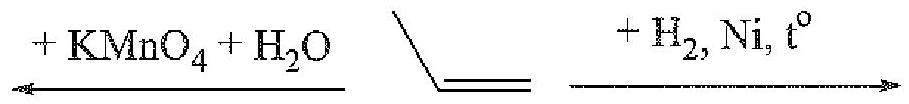
\includegraphics[max width=\textwidth, center]{2025_10_23_fa9073eecee116ad8cf2g-55}\\
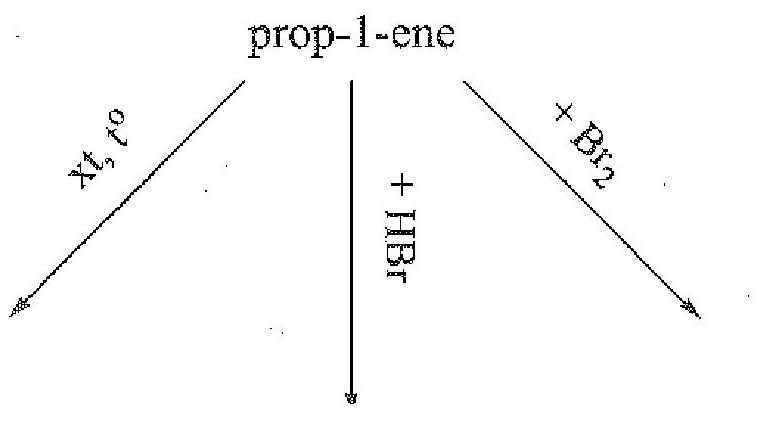
\includegraphics[max width=\textwidth, center]{2025_10_23_fa9073eecee116ad8cf2g-55(1)}\\
16. 16. Dự đoán sản phẩm chính cho mỗi phản úmg sau đây và gọi tên các sản phẩm đó.\\
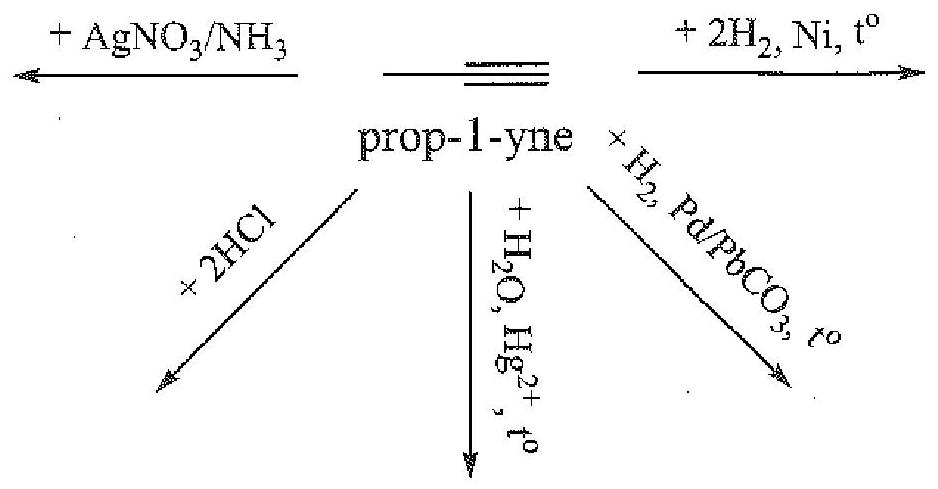
\includegraphics[max width=\textwidth, center]{2025_10_23_fa9073eecee116ad8cf2g-56}\\
16.17. Dự đoán các chất $\mathrm{A}, \mathrm{B}, \mathrm{C}$ và D trong sơ đồ chuyển hoá điều chế poly(vinyl chloride) sau đây và viết các phương trình hoá học.\\
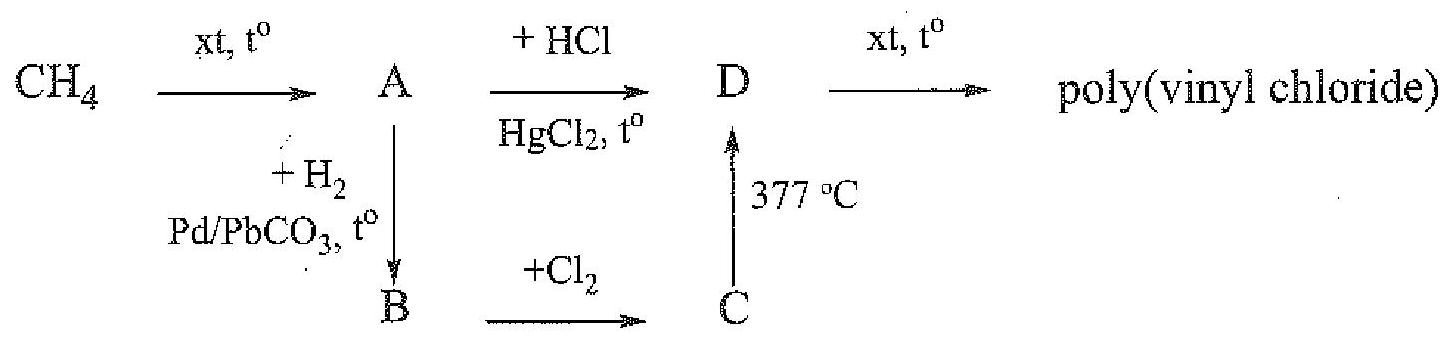
\includegraphics[max width=\textwidth, center]{2025_10_23_fa9073eecee116ad8cf2g-56(1)}

\section*{BÀI 17}
\section*{AREN (HYDROCARBON THOM)}
\section*{NHAM BIST}
17.1. Arene hay còn gọi là hydrocarbon thơm là những hydrocarbon trong phân tử có chứa một hay nhiều\\
A. vòng benzene.\\
B. liên kết đơn.\\
C. liên kết đôi.\\
D. liên kết ba.\\
17.2. Công thức phân tử nào sau đây có thể là công thức của hợp chất thuộc dãy đồng đằng của benzene?\\
A. $\mathrm{C}_{8} \mathrm{H}_{16}$.\\
B. $\mathrm{C}_{8} \mathrm{H}_{14^{\text {a }}}$\\
C. $\mathrm{C}_{8} \mathrm{H}_{12}$.\\
D. $\mathrm{C}_{8} \mathrm{H}_{10}$.\\
17.3. Nhận định nào sau đây về cấu tạo của phân tử benzene không đúng?\\
A. Phân tử benzene có 6 nguyên từ carbon tạo thành hình lục giác đều.\\
B. Tất cả nguyên tử carbon và hydrogen đều nằm trên một mặt phẳng.\\
C. Các góc liên kết đều bằng $109,5^{\circ}$.\\
D. Các độ dài liên kết carbon - carbon đều bằng nhau.\\
17.4. Chất nào sau đây là chất rắn, màu trắng?\\
A. Benzene.\\
B. Toluene.\\
C. Styrene.\\
D. Naphthalene.\\
17.5. Cho các chất sau: (X) o-bromotoluene; (Y) $m$-bromotoluene;\\
(Z) $p$-bromotoluene.

Sản phẩm chỉnh của phản ứng giữa toluen với bromine ở nhiệt độ cao có mặt iron(III) bromide là\\
A. $(\mathrm{X})$ và $(\mathrm{Y})$.\\
B. (Y) và (Z).\\
C. $(\mathrm{X})$ và (Z).\\
D. $(Y)$.\\
17.6. Nitro hoá benzene bằng hỗn hợp $\mathrm{HNO}_{3}$ đặc và $\mathrm{H}_{2} \mathrm{SO}_{4}$ đặc ở nhiệt độ $\leq 50^{\circ} \mathrm{C}$, tạo thành chất hữu $\operatorname{co} \mathrm{X}$.\\
Phát biểu nào sau đây về X không đúng?\\
A. Tên của X là nitrobenzene,\\
B. X là chất lỏng, sánh như dầu.\\
$\mathrm{C} . \mathrm{X}$ có màu vàng.\\
D. $X$ tan tốt trong nước.\\
17.7. Nhận xét nào sau đây không đúng đối với phản ứng cộng chlorine vào benzene?\\
A. Khó hơn phản ứng cộng chlorine vào ethylene.\\
B. Xảy ra với điều kiện ánh sáng tử ngoại và đun nóng.\\
C. Sản phẩm thu được là $1,2,3,4,5,6$-hexachlorocyclohexane.\\
D. Tỉ lệ mol của các chất tham gia phản úng là $1: 1$.\\
17.8. Nhận xét nào sau đây về tính chất hoá học của benzene là không đúng?\\
A. Benzene khó tham gia phản ứng cộng hon ethylene.\\
B. Benzene dễ tham gia phản ứng thế hơn so với phản ứng cộng.\\
C. Benzene không bị oxi hoá bởi tác nhân oxi hoá thông thường.\\
D. Benzene làm mất màu dung dịch nước bromine ở điều kiện thường.

\section*{THONT HILU}
17.9. Phân tứ chất nào sau đây có thể cộng thêm 5 phân tử $\mathrm{H}_{2}$ (xúc tác Ni , đun nóng)?\\
A. Benzene.\\
B. Toluene.\\
C. Styrene.\\
D. Naphthalene.\\
17.10. Chất nào sau đây có thể làm nhạt màu dung dịch $\mathrm{Br}_{2}$ trong $\mathrm{CCl}_{4}$ ở điều kiện thường?\\
A. Benzene.\\
B. Toluene.\\
C. Styrene.\\
D. Naphthalene.\\
17.11. Chất nào sau đây khi tác dụng với hỗn họp $\mathrm{HNO}_{3}$ và $\mathrm{H}_{2} \mathrm{SO}_{4}$ đặc nóng tạo một sản phẩm mononitro hoá duy nhất?\\
A. Benzene.\\
B. Toluene.\\
C. o-xylene.\\
D. Naphthalene.\\
17.12. Phản úng giữa toluene và chlorine khi được chiếu sáng tạo sản phẩm là\\
A. $p$-chlorotoluene.\\
B. $m$-chlorotoluene.\\
C. benzyl chloride.\\
D. 2,4-dichlorotoluene.\\
17.13. Dun nóng toluene với dung dịch $\mathrm{KMnO}_{4}$ nóng, thì ti lệ mol $\mathrm{C}_{6} \mathrm{H}_{5} \mathrm{COOK}$ sinh ra so với $\mathrm{KMnO}_{4}$ phản úng bằng\\
A. $1: 2$.\\
B. $2: 1$.\\
C. 2 : 3 .\\
D. $3: 2$.\\
17.14. Dun nóng hydrocarbon thom X có công thức phân tử $\mathrm{C}_{8} \mathrm{H}_{10}$ với dung dịch $\mathrm{KMnO}_{4}$ nóng thu được dung dịch có chứa $\mathrm{C}_{6} \mathrm{H}_{5} \mathrm{COOK}$ và $\mathrm{K}_{2} \mathrm{CO}_{3}$. Chất X là\\
A. o-xylene.\\
B. $p$-xylene.\\
C. ethyl benzene.\\
D. styrene.\\
17.15. Viết đồng phân và goi tên các arene có cùng công thức phân tử $\mathrm{C}_{8} \mathrm{H}_{10}$.

\section*{VAN DUNG}
17.16. Cho 40 mL dung dịch $\mathrm{H}_{2} \mathrm{SO}_{4}$ đặc, lạnh vào bình cầu đang được giữ lạnh, thêm 35 mL dung dịch $\mathrm{HNO}_{3}$ đăc. Sau đó, thêm từ từ 30 mL benzene và khuấy đều (giữ nhiệt độ trong khoảng $55-60^{\circ} \mathrm{C}$ ). Sau khoảng một giờ thu được lớp chất lòng X màu vàng, không tan trong nước và nhẹ hơn nước.\\
Xác định chất X và viết phương trình hoá học.\\
17.17. Biết nhóm thế - Br trên vòng benzene định hướng thế ưu tiên các vị trí ortho và para, còn nhóm thế - $\mathrm{NO}_{2}$ trên vòng benzene định hướng thế vào vị trí meta. Hãy xác định cấu tạo và tên gọi của các chất còn thiếu trong mỗi sơ đồ chuyển hoá sau đây (mỗi phản ứng chỉ xảy ra một lần thế và các chất còn thiếu là sản phẩm chính của phản ưng).\\
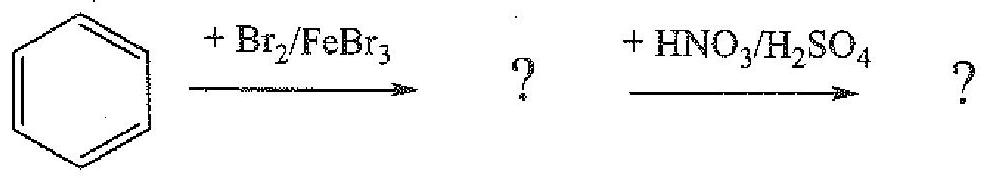
\includegraphics[max width=\textwidth, center]{2025_10_23_fa9073eecee116ad8cf2g-59(2)}\\
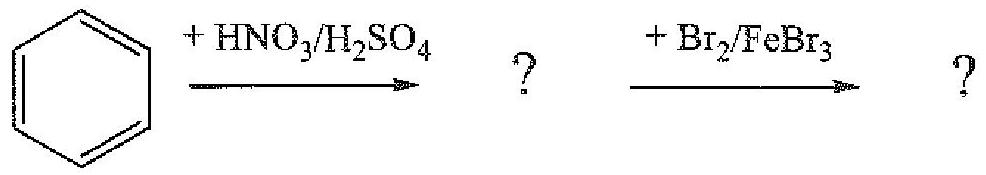
\includegraphics[max width=\textwidth, center]{2025_10_23_fa9073eecee116ad8cf2g-59}\\
17.18. Dự đoán sản phẩm chính của mỗi phản ứng trong sơ đồ sau và gọi tên các sản phẩm đó.\\
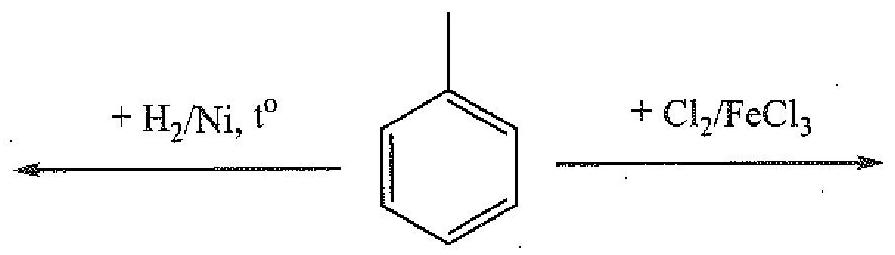
\includegraphics[max width=\textwidth, center]{2025_10_23_fa9073eecee116ad8cf2g-59(4)}\\
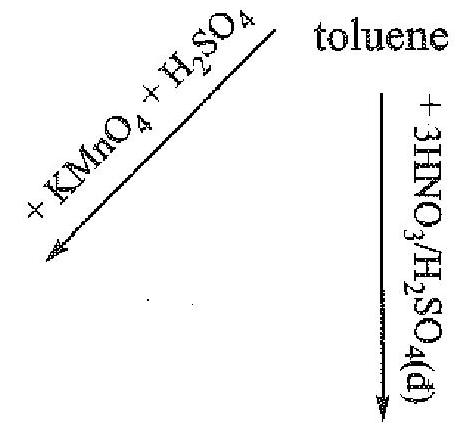
\includegraphics[max width=\textwidth, center]{2025_10_23_fa9073eecee116ad8cf2g-59(1)}\\
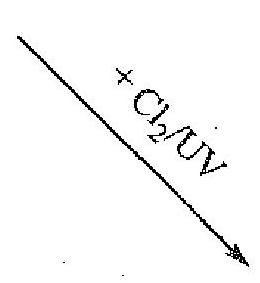
\includegraphics[max width=\textwidth, center]{2025_10_23_fa9073eecee116ad8cf2g-59(3)}\\
17.19. Viết các phương trình phản ứng minh hoạ các quá trình điều chế:\\
a) Polystyrene từ hexane.\\
b) 2,4,6-trinitrotoluene từ heptane.

\section*{BÀl 18}
\section*{ÔN TẬP CHUONG 4}
\section*{NHAN BIST}
18.1. Chất nào sau đây không phải là hydrocarbon?\\
A. $\mathrm{CH}_{3}-\mathrm{CH}_{3}$.\\
B. $\mathrm{CH}_{2}=\mathrm{CH}_{2}$.\\
C. $\mathrm{CH}=\mathrm{CH}$.\\
D. $\mathrm{CH}_{3}-\mathrm{CH}_{2}-\mathrm{OH}$.\\
18.2. Cho các hydrocarbon sau:\\
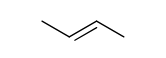
\includegraphics{smile-125fc74a40ef3561e9e0b939a344656fc770676e}\\
\includegraphics{smile-13b100b8888d222ef7dd5acee0aebb7e05e452df}\\
\includegraphics{smile-57328846cad84dd225af1bff9432f8ba9af23479}\\
\includegraphics{smile-c69a8eae60cd42899bc6b56ffc474be9f3600368}\\
\includegraphics{smile-04c8fbf978c86cc6929fa571e361d8b3a4133d11}\\
\includegraphics{smile-0e8d654a3e708708ef21429308cb866e00564526}\\
\includegraphics{smile-bca0308d7ac35b51496ad782213b5a2609a44648}\\
\includegraphics{smile-97b9ce6d965dabd632e639456cb629f0748f3017}\\
\includegraphics{smile-fbd09d2e2e2df96f7d77f19e65d31cfe800c64ba}\\
\includegraphics{smile-9efbb27159cf7c9bc191dd8248bcf704989a6fae}\\
\includegraphics{smile-a62a4bab4c17ae5d2e92863179a60f58c7dd4350}

Một số nhận định về các hydrocarbon trên là:\\
(1) Số phân tử hydrocarbon không no bằng 5;\\
(2) Số phân tữ alkene bằng 3;\\
(3) Số phân tử alkyne bằng 2;\\
(4) số phân tử thuộc dãy đồng đẳng của benzene bằng 3 .

Trong các nhận định này, số nhận định đúng bằng\\
A. 1 .\\
B. 2 .\\
C. 3 .\\
D. 4 .\\
18.3. Tên gọi của chất nào sau đây không đúng?\\
、 $\cdots$\\
A. but-2-ene\\
B. 3-methylbut-1-yne -\\
\includegraphics{smile-73930640eef7b9eb765d174771c78cfb8baa20df}\\
C. 2,2,4-trimethylpentane\\
D. 1-ethyl-2-methylbenzene\\
\includegraphics{smile-fe186c8d4e7046f8eb7f8f139268fbe054ead823}\\
18.4. Cho các chất sau: methane, ethylene, acetylene, benzene, toluene và naphthalene.\\
Số chất ở thể lỏng trong điều kiện thường là\\
A. 1 .\\
B. 2 .\\
C. 3.\\
D. 4 .\\
18.5. Nhận xét nào sau đây không đúng?\\
A. Alkane không tham gia phản ứng cộng.\\
B. Phản ứng đặc trưng của alkene và alkyne là phản ứng công.\\
C. Benzene và đồng đẳng dễ tham gia phản ưng thế hơn phản ứng cộng.\\
D. Styrene dễ tham gia phản ứng thế hơn phản ứng cộng.

\section*{THONO HILU}
18.6. Hợp chất X có công thức phân tử $\mathrm{C}_{5} \mathrm{H}_{12}$, khi tác dụng với chlorine (có chiếu sáng) tạo được bốn đẫn xuất thế monochlorine. X là\\
A. pentane.\\
B. isopentane.\\
C. neopentane.\\
D. isobutane.\\
18.7. Chất lỏng X có khả năng làm nhạt màu dung dịch $\mathrm{KMnO}_{4}$ ở điều kiện thường. X là chất nào trong các chất sau đây?\\
A. Benzene.\\
B. Toluene.\\
C. Styrene.\\
D. Naphtalene.\\
18.8. Cho các chất sau: propane, propene, propyne, butane, but-1-yne, but-2-yne, but-1-ene và cis-but-2-ene.\\
Số chất tác dụng với dung dịch $\mathrm{AgNO}_{3}$ trong $\mathrm{NH}_{3}$ tạo kết tủa là\\
A. 1 .\\
B. 2 .\\
C. 3 .\\
D. 4 .\\
18.9. Cho các phát biểu sau:\\
(1) Propane và butane được sử dụng làm khí đốt;\\
(2) Ethene và propene đượ sử dụng để tồng họp polymer;\\
(3) Acetylene được sứ dụng làm nhiên liệu cho đèn xì oxygen-acetylene;\\
(4) Styrene được sử dụng tổng hợp polymer;\\
(5) Toluene được sử dụng tổng hợp thuốc nổ.

Số phát biểu đúng là\\
A. 5 .\\
B. 2 .\\
C. 3 .\\
D. 4 .\\
18.10. a) Cho các hydrocarbon sau: ethane, ethylene, acetylene, butane, benzene, styrene và naphthalene.\\
Cho biết trạng thái của các hydrocarbon trên ở điều kiện thường.\\
b) Tại sao các hydrocarbon không tan hoặc it tan trong nước nhưng tan nhiều trong các dung môi hữu cơ?

\section*{VAN DUING}
18.11. Viết đồng phân và gọi tên các alkane, alkene, alkyne có 5 nguyên tử carbon trong phân tữ và đồng đẳng của benzene có 8 nguyên tữ carbon trong phân tử.\\
18.12. Hoàn thành sơ đồ chuyển hoá sau đây và viết các phương trình hoá học.\\
A\\
(1) $\mid+\mathrm{Cl}_{2}$, as (ti lệ $1: 1$ )\\
C\\
(4) $\stackrel{t}{\dagger}+\mathrm{HCl}, \mathrm{Hg}^{2+}, \mathrm{t}^{\circ}$\\
F\\
(7) $\mid+\mathrm{H}_{2} \mathrm{O}, \mathrm{H}^{+}, \mathrm{t}^{\circ}$\\
$\mathrm{CH}_{4}$\\
$\xrightarrow[\text { (3) }]{ }$\\
$\mathrm{HC} \equiv \mathrm{CH}$\\
$\longrightarrow$\\
(6)\\
E\\
$\longrightarrow$ Polyethylene\\
(2) $\mid+\mathrm{O}_{2}, \mathrm{t}^{\circ}$\\
B\\
(5) $\mid+\mathrm{H}_{2} \mathrm{O}, \mathrm{Hg}^{2+}, \mathrm{t}^{\circ}$\\
D\\
(8) $\mid+\mathrm{KMnO}_{4}+\mathrm{H}_{2} \mathrm{O}$\\
G\\
18.13. Hoàn thành sơ đồ chuyển hoá sau đây và viết các phương trình hoá học. (Biết $\mathrm{A}, \mathrm{B}, \mathrm{C}, \mathrm{D}, \mathrm{D}, \mathrm{F}$ là các sản phẩm chính)\\
\includegraphics[max width=\textwidth, center]{2025_10_23_fa9073eecee116ad8cf2g-62(1)}

C

\begin{figure}[h]
\begin{center}
  \includegraphics[width=\textwidth]{2025_10_23_fa9073eecee116ad8cf2g-62}
\captionsetup{labelformat=empty}
\caption{(4)}
\end{center}
\end{figure}

(5)

$$
\text { (7) }+\begin{gathered}
+\mathrm{HNO}_{3} / \mathrm{H}_{2} \mathrm{SO}_{4} \\
(\mathrm{ti} \mathrm{ệ} 1: 2)
\end{gathered}
$$

D

\section*{Chưong 5 \\
 DAN XUAT IALOGEN ALCOHOL - PLIENOL }
\section*{BÀ 19}
\section*{DẪN XUẤT HALOGEN}
\section*{NHAN DIET}
19.1. Công thức tổng quát của dẫn xuất monochlorine no, mạch hở là:\\
A. $\mathrm{C}_{\mathrm{n}} \mathrm{H}_{2 \mathrm{n}-5} \mathrm{Cl}$.\\
B. $\mathrm{C}_{n} \mathrm{H}_{2 n-3} \mathrm{Cl}$.\\
C. $\mathrm{C}_{\mathrm{n}} \mathrm{H}_{2 \mathrm{n}-1} \mathrm{Cl}$.\\
D. $\mathrm{C}_{n} \mathrm{H}_{2 n+1} \mathrm{Cl}$.\\
19.2. Tên goi theo danh pháp thay thế của dẫn xuất halogen có công thức cấu tạo $\mathrm{CH}_{3} \mathrm{CHClCH}_{3}$ là\\
A. 1-chloropropane.\\
B. 2-chloropropane.\\
C. 3 -chloropropane.\\
D. propyl chloride.\\
19.3. Dẫn xuất halogen nào sau đây có đồng phân hình học?\\
A. $\mathrm{CH}_{2}=\mathrm{CHCl}$.\\
B. $\mathrm{CH}_{2}=\mathrm{CH}-\mathrm{CH}_{2} \mathrm{Br}$.\\
C. $\mathrm{CH}_{3} \mathrm{CH}=\mathrm{CFCH}_{3}$.\\
D. $\left(\mathrm{CH}_{3}\right)_{2} \mathrm{C}=\mathrm{CHI}$.\\
19.4. Cho các dẫn xuất halogen sau:\\
(1) $\mathrm{C}_{2} \mathrm{H}_{5} \mathrm{~F}$;\\
(2) $\mathrm{C}_{2} \mathrm{H}_{5} \mathrm{Cl}$;\\
(3) $\mathrm{C}_{2} \mathrm{H}_{5} \mathrm{Br}$;\\
(4) $\mathrm{C}_{2} \mathrm{H}_{5} \mathrm{I}$.

Thứ tự giảm dần nhiệt độ sôi là\\
A. $(1)>(2)>(3)>(4)$.\\
B. $(1)>(4)>(2)>(3)$.\\
C. $(4)>(3)>(2)>(1)$.\\
D. $(4)>(2)>(1)>(3)$.\\
19.5. Cho phản úng hoá học sau:\\
$\mathrm{C}_{2} \mathrm{H}_{5}-\mathrm{Br}+\mathrm{NaOH} \xrightarrow{t^{\circ}} \mathrm{C}_{2} \mathrm{H}_{5}-\mathrm{OH}+\mathrm{NaBr}$\\
Phản ứng trên thuộc loại phản ứng nào sau đây?\\
A. Phản ứng thế.\\
B. Phản ứng cộng.\\
C. Phản ứng tách.\\
D. Phản ứng oxi hoá - khử.\\
19.6. Cho so đồ phản ứng hoá học sau:\\
$\mathrm{CH}_{3} \mathrm{CHClCH}_{2} \mathrm{CH}_{3} \xrightarrow{\mathrm{NaOH}_{3} \mathrm{C}_{2} \mathrm{H}_{5} \mathrm{OH}_{4} \mathrm{t}^{\circ}}$ ?\\
Sản phẩm chính theo quy tắc Zaitsev của phản úng trên là\\
A. but-1-ene.\\
B. but-2-ene.\\
C. but-1-yne.\\
D. but-2-yne.\\
19.7. Chất nào sau đây không phải là dẫn xuất halogen của hydrocarbon?\\
A. $\mathrm{CH}_{3} \mathrm{CH}_{2} \mathrm{Cl}$.\\
B. $\mathrm{CH}_{2}=\mathrm{CHBr}$.\\
C. $\mathrm{ClCH}_{2} \mathrm{COOH}$.\\
D. $\mathrm{CF}_{3} \mathrm{CH}_{2} \mathrm{Cl}$.

\section*{THONG HILU}
19.8. Cho dẫn xuất halogen có công thức cấu tạo sau:\\
\includegraphics{smile-1f2915d88567dae8b01377510c65280023e96568}

Danh pháp thay thế của dẫn xuất halogen trên là\\
A. 3,4-dimethyl-2-chlorohexane.\\
B. 2-chloro-3,4-dimethylhexane.\\
C. 3,4-dimethyl-5-chlorohexane.\\
D. 5-chloro-3,4-dimethylhexane.\\
19.9. Nhận xét nào sau đây không đúng?\\
A. Dận xuất halogen có nhiệt độ sôi và nhiệt độ nóng chảy cao hơn hydrocarbon có phân tử khối tương đương.\\
B. Thử phân ethyl bromide trong môi trường kiềm thu được ethyl alcohol.\\
C. Phản ứng tách HCl của 2 -chloropropane chỉ thu được một alkene duy nhất.\\
D. CFC là hợp chất chứa các nguyên tố carbon, fluorine, chlorine và hydrogen.\\
19.10. Sån phẩm chính theo quy tắc Zaitsev của phản ứng tách HCl ra khỏi phân tử 2-chloro-3-methyl butane là\\
A. 2-methylbut-2-ene.\\
B. 3-methylbut-2-ene.\\
C. 3-methylbut-3-ene.\\
D. 2-methylbut-3-ene.\\
19.11. Đun nóng $\mathrm{CH}_{2}=\mathrm{CHCH}_{2} \mathrm{Br}$ với dung dịch kiềm, trung hoà hỗn hợp thu được bằng dung dịch $\mathrm{HNO}_{3}$. Nhỏ vài giọt dung dịch $\mathrm{AgNO}_{3}$ vào ống nghiệm và lấc nhẹ thấy có kết tủa màu vàng nhạt xuât hiện. Hãy giải thích hiện tượng xảy ra.\\
19.12. R-45B là một chất làm lạnh thế hệ mới sẽ thay thế các chất làm lạnh không thân thiện với môi trường, ảnh hưởng đến tầng ozone. R-45B chứa hỗn họp gồm difluoromethane và $2,3,3,3$-tetrafluoropropene. Hãy viết công thức cấu tạo các dẫn xuất halogen có trong R-45B.

\section*{VANT DUNG}
19.13. a) Viết các đồng phân cấu tạo có thể có của các dẫn xuất halogen có công thức phân tự $\mathrm{C}_{4} \mathrm{H}_{9} \mathrm{Br}$.\\
b) Thực hiện phản ứng tách HBr một trong các chất trên thu được hai alkene. Xác định công thức của dẫn xuất halogen đó.\\
19.14. Cho sơ đồ phản ứng sau:\\
\includegraphics[max width=\textwidth, center]{2025_10_23_fa9073eecee116ad8cf2g-65}\\
a) Viết các phương trình hoá học để hoàn thành sơ đồ phản ứng trên.\\
b) Nếu thay ethylene bằng but-1-ene thì sản phẩm chính thu được ở các phản ứng trên sẽ như thế nào?\\
19.15. Đun nóng hợp chất A có công thức phân tử $\mathrm{C}_{5} \mathrm{H}_{11} \mathrm{Br}$ trong môi trường kiềm và ethanol, thu được sản phẩm chính là 2 -methylbut-2-ene. Hãy xác định các công thức cấu tạo có thể có của A .

\section*{BÀI 20}
\section*{ALCOHOL}
\section*{NHAN DILT}
20.1. Công thức tổng quát của alcohol no, đơn chực, mạch hở là\\
A. $\mathrm{C}_{n} \mathrm{H}_{2 n-5} \mathrm{OH}$.\\
B. $\mathrm{C}_{\mathrm{n}} \mathrm{H}_{2 \mathrm{n}}(\mathrm{OH})_{2}$.\\
C. $\mathrm{C}_{\mathrm{n}} \mathrm{H}_{2 \mathrm{n}-1} \mathrm{OH}$.\\
D. $\mathrm{C}_{\mathrm{n}} \mathrm{H}_{2 \mathrm{n}+1} \mathrm{OH}$.\\
20.2. Số đồng phân cấu tạo alcohol có công thức $\mathrm{C}_{4} \mathrm{H}_{9} \mathrm{OH}$ là\\
A. 2 .\\
B. 3 .\\
C. 4 .\\
D. 5 .\\
20.3. Chất nào sau đây là alcohol bậc II?\\
A. propan-1-ol.\\
B. propan-2-ol.\\
C. 2-methylpropan-1-ol.\\
D. 2-methylpropan-2-ol.\\
20.4. Cho alcohol có công thức cấu tạo sau:\\
\includegraphics{smile-c525e1c8da27cbaa0cdb7e4b9de47a1770dd88f7}

Tên theo danh pháp thay thế của alcohol đó là\\
A. 4-methylpentan-1-ol.\\
B. 2-methylbutan-3-ol.\\
C. 3-methylbutan-2-ol.\\
D. 1,1-dimethylpropan-3-ol.\\
20.5. Nhiều vụ ngộ độc rượu do sử dụng rượu được pha chế từ cồn công nghiệp có lẫn methanol. Cong thức phân tứ của methanol là\\
A. $\mathrm{CH}_{3} \mathrm{OH}$.\\
B. $\mathrm{C}_{2} \mathrm{H}_{5} \mathrm{OH}$.\\
C. $\mathrm{C}_{3} \mathrm{H}_{7} \mathrm{OH}$.\\
D. $\mathrm{C}_{2} \mathrm{H}_{4}(\mathrm{OH})_{2}$.\\
20.6. Cho các hợp chất hữu cơ sau:\\
(1) $\mathrm{C}_{3} \mathrm{H}_{8}$;\\
(2) $\mathrm{CH}_{3} \mathrm{Cl}$;\\
(3) $\mathrm{C}_{2} \mathrm{H}_{5} \mathrm{OH}$;\\
(4) $\mathrm{CH}_{3} \mathrm{OH}$.

Thứ tự giảm dần nhiệt độ sôi của các chất trên là\\
A. $(1)>(2)>(3)>(4)$.\\
B. $(1)>(4)>(2)>(3)$.\\
C. $(3)>(4)>(2)>(1)$.\\
D. $(4)>(2)>(1)>(3)$.\\
20.7. Để pha chế một loại cồn sát trùng sử dụng trong y tế, người ta cho 700 mL ethanol nguyên chất vào bình định mức rồi thêm nước cất vào, thu được 1000 mL cồn. Hỗn hợp trên có độ cồn là\\
A. $17^{\circ}$.\\
B. $7^{\circ}$.\\
C. $70^{\circ}$.\\
D. $170^{\circ}$.\\
20.8. Số họp chất hữu cơ có công thức phân tử. $\mathrm{C}_{3} \mathrm{H}_{8} \mathrm{O}$ phản ứng được với Na là\\
A. 1 .\\
B. 2 .\\
C. 3 .\\
D. 4 .\\
20.9. Cho phản ứng hoá học sau: $\mathrm{CH}_{3} \mathrm{CHOHCH}_{2} \mathrm{CH}_{3} \xrightarrow{\mathrm{H}_{2} \mathrm{SO}_{4}, \mathrm{t}^{\circ}}$ ?

Sản phẩm chính theo quy tắc Zaitsev trong phản úng trên là\\
A. but-1-ene.\\
B. but-2-ene.\\
C, but-1-yne.\\
D. but-2-yne.\\
20.10. Oxí hoá propan-2-ol bằng CuO nung nóng, thu được sàn phẩm nào sau đây?\\
A. $\mathrm{CH}_{3} \mathrm{CHO}$.\\
B. $\mathrm{CH}_{3} \mathrm{CH}_{2} \mathrm{CHO}$.\\
C. $\mathrm{CH}_{3} \mathrm{COCH}_{3}$.\\
D. $\mathrm{CH}_{3} \mathrm{COOH}$.\\
20.11. Thuốc thử $\mathrm{Cu}(\mathrm{OH})_{2}$ dùng để nhận biết alcohol nào sau đây?\\
A. Alcohol bậc I.\\
B. Alcohol bậc II.\\
C. Alcohol bậc III.\\
D. Alcohol đa chức.\\
20.12. Khi đốt cháy hoàn toàn ethanol, thu được tỉ lẹ mol $\mathrm{n}_{\mathrm{CO}_{2}}: \mathrm{n}_{\mathrm{H}_{2} \mathrm{O}}$ là\\
A. $1: 1$.\\
B. $1: 2$.\\
C. 2 : 3 .\\
D. $3: 2$.\\
20.13. Chất nào sau đây dùng để điều chế ethanol theo phương pháp sinh hoá?\\
A. Ethylene.\\
B. Acetylene.\\
C. Methane.\\
D. Tinh bột.\\
20.14. Để phân biệt cồn $90^{\circ}$ và cồn tuyệt đối (ethanol nguyên chất), có thể dùng hoá chất nào sau đây?\\
A. Na.\\
B. $\mathrm{CuSO}_{4}$ khan.\\
C. $\mathrm{CuO}, t^{\circ}$.\\
D. $\mathrm{Cu}(\mathrm{OH})_{2}$.

\section*{THONG HELU}
20.15. Hai ancol nào sau đây cùng bậc?\\
A. Methanol và ethanol.\\
B. Propan-1-ol và propan-2-ol.\\
C. Ethanol và propan-2-ol.\\
D. Propan-2-ol và 2-methylpropan-2-ol,\\
20.16. Alcohol $\mathrm{CH}_{3} \mathrm{CH}=\mathrm{CHCH}_{2} \mathrm{OH}$ có danh pháp thay thế là\\
A. but-2-en-4-ol.\\
B. but-2-en-1-ol.\\
C. 4-bydroxybut-2-ene.\\
D. 1-hydroxybut-2-ene.\\
20.17. Một học sinh sau khi tiến hành thí nghiệm thì vẫn còn dư mẩu Na. Để tiêu huỷ mẩu Na dư này một cách an toàn, học sinh đó nên cho mẩu Na vào\\
A. nước.\\
B. cồn $96^{\circ}$.\\
C. thùng rác.\\
D. dầu hoả.\\
20.18. Một chai rượu gạo có thể tích 750 mL và có độ rượu là $40^{\circ}$. Số mL ethanol nguyên chất (khan) có trong chai rượu đó là\\
A. $18,75 \mathrm{~mL}$.\\
B. 300 mL .\\
C. 400 mL .\\
D. 750 mL .\\
20.19. Xăng E 5 chứa $5 \%$ thể tích ethanol hiện đang được sử dựng phổ biến ở nước ta để thay thế một phần xăng thông thường. Một người đi xe máy mua 2 L xăng E5 để đổ vào bình chứa nhiên liệu. Thể tích ethanol có trong lương xăng trên là\\
A. 50 mL .\\
B. 92 mL .\\
C. 46 mL .\\
D. 100 mL .\\
20.20. Cho các alcohol sau:\\
\includegraphics{smile-05b745ac0f9a73f4cb25e4e2db75e13930d66c15}

Số alcohol khồng hoà tan được $\mathrm{Cu}(\mathrm{OH})_{2}$ là\\
A. 1 .\\
B. 2.\\
C. 3 .\\
D. 4 .\\
20.21. Nhận xét nào sau đây không đúng?\\
A. Oxi hoá không hoàn toàn alcohol bậc I, thu được aldehyde.\\
B. Oxi hoá hoàn toàn alcohol bậc I, thu được aldehyde.\\
C. Oxi hoá alcohol bạc II, thu được ketone.\\
D. Alcohol bậc III không bị oxì hoá bởi tác nhân thông thường.\\
20.22. Sản phẩm chính thu được khi tách nước từ 3-methylbutan-2-ol là\\
A. 3-metylbut-1-ene.\\
B. 2-methylbut-2-ene.\\
C. 3-methylbut-2-ene.\\
D. 2-methylbut-3-ene.\\
20.23. Oxi hoá alcohol nào sau đây thu được sản phẩm là ketone?\\
A. $\mathrm{C}_{2} \mathrm{H}_{5} \mathrm{OH}$.\\
B. $\mathrm{CH}_{3} \mathrm{CH}_{2} \mathrm{CH}_{2} \mathrm{OH}$.\\
C. $\mathrm{CH}_{3} \mathrm{CH}(\mathrm{OH}) \mathrm{CH}_{3}$.\\
D. $\left(\mathrm{CH}_{3}\right)_{2} \mathrm{C}(\mathrm{OH}) \mathrm{CH}_{3}$.\\
20.24. Phương pháp nào sau đây dùng để sản xuất ethanol sinh học?\\
A. Cho hỗn hợp khí ethylene và hơi nước đi qua tháp chứa $\mathrm{H}_{3} \mathrm{PO}_{4}$.\\
B. Cộng nước vào ethylene với xúc tác là $\mathrm{H}_{2} \mathrm{SO}_{4}$.\\
C. Lên men tinh bột.\\
D. Thuỷ phân dẫn xuất $\mathrm{C}_{2} \mathrm{H}_{5} \mathrm{Br}$ trong môi trường kiềm.\\
20.25. Cho dãy chuyển hoá sau:\\
\includegraphics[max width=\textwidth, center]{2025_10_23_fa9073eecee116ad8cf2g-68}

Biết $X$ và $Y$ đều là sản phẩm chính, công thức cấu tạo của $X, Y$ lần lượt là\\
A. $\mathrm{CH}_{3} \mathrm{CH}=\mathrm{CHCH}_{3}$ và $\mathrm{CH}_{3} \mathrm{CH}_{2} \mathrm{CHBrCH}_{3}$.\\
B. $\mathrm{C}_{4} \mathrm{H}_{9}-\mathrm{O}-\mathrm{C}_{4} \mathrm{H}_{9}$ và $\mathrm{CH}_{3} \mathrm{CH}_{2} \mathrm{CHBrCH}_{3}$.\\
C. $\mathrm{CH}_{2}=\mathrm{CHCH}_{2} \mathrm{CH}_{3}$ và $\mathrm{CH}_{3} \mathrm{CH}_{2} \mathrm{CHBrCH}_{3}$.\\
D. $\mathrm{CH}_{2}=\mathrm{CHCH}_{2} \mathrm{CH}_{3}$ và $\mathrm{CH}_{3} \mathrm{CH}_{2} \mathrm{CH}_{2} \mathrm{CH}_{2} \mathrm{Br}$.\\
20.26. a) Viết các đồng phân cấu tạo alcohol bậc I có công thức $\mathrm{C}_{5} \mathrm{H}_{11} \mathrm{OH}$.\\
b) Đun nóng một trong các alcohol trên với $\mathrm{H}_{2} \mathrm{SO}_{4}$ đặc, thu được alkene có tên gọi là 3-methylbut-1-ene, xác dịnh công thức của alcohol đó.\\
20.27. Một học sinh tiến hành thí nghiệm như sau: Lấy một mẩu nhỏ Na vào cốc chứa ethanol dư, thấy mầu Na tan dần và có sủi bọt khí. Sau khi kết thúc phản ứng thấy có kết tủa trắng xuất hiện, thêm một ît nưởc vào dung dịch sau phản ứng thấy kết tủa tan. Nhó vài giọt phenolphtalein vào dung dịch thu được, thấy dung dịch chuyển thành màu hồng. Giải thích các hiện tượg trên và viết phương trình hoá học của phản ứng xảy ra.

\section*{VANIOUMG}
20.28. Thí nghiệm theo sơ đồ sau đây được dùng để điều chế một lượng nhỏ ethylene trong phòng thí nghiệm.\\
\includegraphics[max width=\textwidth, center]{2025_10_23_fa9073eecee116ad8cf2g-69}\\
a) Viết phương trình hoá học của phản úng xảy ra.\\
b) Tại sao lại dùng phương pháp đẩy nước đề thu khí ethylene.\\
c) Nêu tác dưng của bông tẩm dung dịch NaOH .\\
d) Đề xuất thí nghiệm để nhận biết khí tạo thành.\\
20.29. Tính lượng glucose cần lên men để sản xuất 100 L cồn y tế $70^{\circ}$, biết hiệu suất của quá trình lên men là $80 \%$, khối lượng riêng của ethanol là $0,789 \mathrm{~g} / \mathrm{mL}$.\\
20.30. Một đèn cồn thí nghiệm chứa 100 mL cồn $90^{\circ}$. Tính nhiệt lượng đèn cồn toả ra khi đốt cháy hết lượng cồn trên, biết khối lượng riêng của ethanol là $0,789 \mathrm{~g} / \mathrm{mL}$ và nhiệt sinh ra khi đốt cháy 1 mol ethanol là $1371 \mathrm{~kJ} \cdot \mathrm{~mol}^{-1}$.\\
20.31. Hợp chất X có tác dụng kháng khuẩn, chống vi sinh vật kí sinh trên da (chấy, rận,...). X có công thức phân tử $\mathrm{C}_{7} \mathrm{H}_{8} \mathrm{O}$ và có chứa vòng benzene, phổ $\mathbb{R}$ của X có peak hấp thự rộng ở vừng $3300 \mathrm{~cm}^{-1}$. Oxi hoá X bằng CuO nung nóng, thu được hợp chất Y có peak hấp thụ đặc trưng ở khoảng $1700 \mathrm{~cm}^{-1}$. Xác định công thức cấu tạo của $X, Y$ và viết phương trình hoá học của phản ứng xảy ra.\\
20.32. Từ 1 tấn tinh bột ngô có thể sản xuất được bao nhiêu lít xăng E 5 (chứa $5 \%$ ethanol về thể tích), biết tinh bột ngô chưa $75 \%$ tinh bột, hiệu suất chung của cả quá trình điều chế ethanol là $70 \%$, khối lượng riêng của ethanol 1 à $0,789 \mathrm{~g} / \mathrm{mL}$.

\section*{BÀI 21}
\section*{PHENOL}
\section*{WHAT BTÉT}
21.1. Phenol là hợp chất hữu $c o$, trong phân tử có\\
A. nhóm -OH và vòng benzene.\\
B. nhóm -OH liên kết trực tiếp với nguyên tử carbon của vòng benzene.\\
C. nhóm -OH liên kết trực tiếp với nguyên tử carbon no.\\
D. nhóm -OH liên kết trực tiếp với nguyên tử carbon no và có chứa vòng benzene.\\
21.2. Cho các phát biểu sau về phenol:\\
(1) Phenol tan một phần trong nước ở điều kiện thường.\\
(2) Phenol tan vô hạn trong nước ở điều kiện thường.\\
(3) Phenol tan tốt trong nước khi đun nóng.\\
(4) Nhiệt độ nóng chảy của phenol cao hơn ethanol.\\
(5) Phenol có tính độc và có thể gây bỏng khi tiếp xúc với da nên cần phải cẩn thận khi sử dụng.\\
Số phát biểu đúng là\\
A. 2 .\\
B. 3 .\\
C. 4 .\\
D. 5 .\\
21.3. Hợp chất hữu cơ X có chứa vòng benzene, có công thức phân tử là $\mathrm{C}_{7} \mathrm{H}_{8} \mathrm{O}$. Số đồng phân cấu tạo của X là\\
A. 2 .\\
B. 3 .\\
C. 4.\\
D. 5 .\\
21.4. Phenol là hợp chất hữu cơ có tính\\
A. acid yếu.\\
B. base yếu.\\
C. acid mạnh.\\
D. base manh.\\
21.5. Phản ứng với chất/dung dịch nào sau đây của phenol chứng minh phenol có tinh acid?\\
A. Na.\\
B. Dung dich NaOH .\\
C. Dung dich bromine.\\
D. $\mathrm{HNO}_{3}$ đặc $/ \mathrm{H}_{2} \mathrm{SO}_{4}$ đăc.\\
21.6. Nguyên nhân phản ứng thế bromine vào vòng thơm của phenol xảy ra dễ dàng hon so với benzene là do\\
A. phenol tan một phần trong nước.\\
B. phenol có tính acid yếu.\\
C. ảnh hưởng của nhóm -OH đến vòng benzene trong phân tữ phenol.\\
D. ảnh hưởng của vòng benzene đến nhóm -OH trong phận tử phenol.\\
21.7. Khi nhỏ từ từ dung dịch bromine vào ống nghiệm chưa dung dịch phenol, hiện tượng quan sát được trong ống nghiệm là\\
A. nước brom bị mất màu và xuất hiện kết tủa trắng.\\
B. dung dịch trong suôt.\\
C. xuất hiện kết tủa trắng.\\
D. không xảy ra hiện tượng gì.\\
21.8. Trong công nghiềp, phenol được điều chế chủ yếu từ chất nào sau đây?\\
A. Benzene.\\
B. Cumene.\\
C. Chlorobenzene.\\
D. Than đá.

\section*{THONG HISU}
21.9. Cho hợp chất phenol có công thức cấu tạo sau:\\
\includegraphics{smile-bda674f18e893e4449b65cdf5ade68e2df646f10}

Tên gọi của phenol đó là\\
A. 2-methylphenol.\\
B. 3-methylphenol.\\
C. 4-methylphenol.\\
D. hydroxytoluene.\\
21.10. Phản ứng với chất/dung dịch nào sau đây chứng minh tính acid của phenol ( $\mathrm{C}_{6} \mathrm{H}_{5} \mathrm{OH}$ ) manh hon ethanol?\\
A. Na.\\
B. Dung dịch NaOH .\\
C. Dung dich bromine.\\
D. $\mathrm{HNO}_{3}$ đặc/ $\mathrm{H}_{2} \mathrm{SO}_{4}$ đặc.\\
21.11. Phản ứng với chất/dung dịch nào sau đây chứng minh phenol $\left(\mathrm{C}_{6} \mathrm{H}_{5} \mathrm{OH}\right)$ có tính acid mạnh hơn nấc 2 của carbonic acid?\\
A. Na.\\
B. Dung dich NaOH .\\
C. Dung dịch $\mathrm{Na}_{2} \mathrm{CO}_{3}$.\\
D. Dung dich $\mathrm{Br}_{2}$.\\
21.12. Cho các chất có cùng công thức phân tử $\mathrm{C}_{7} \mathrm{H}_{8} \mathrm{O}$ sau:\\
\includegraphics{smile-ae487b1401f156292ad07e6087b95069188bc895}\\
\includegraphics{smile-6b4ded2887baeb6fa657fcbea88e2be9bae3e764}\\
\includegraphics{smile-8dd3490ec8e20c460ab461a4f6ec6950b9ef5394}\\
\includegraphics{smile-03295b8eae25286a2b11cc9e8eb36935757c277d}

Số chất vừa phản ứng được với Na , vừa phản ứng được với dung dịch NaOH là\\
A. 1 .\\
B. 2 .\\
C. 3 .\\
D. 4 .\\
21.13. Cho các phát biểu sau về phenol $\left(\mathrm{C}_{6} \mathrm{H}_{5} \mathrm{OH}\right)$ :\\
a) Phenol là hợp chất hữu cơ trong phân tử có vòng benzenè và nhóm -OH .\\
b) Do có nhóm -OH nên phenol tan vô hạn trong nước ở điều kiện thường tương tự ethanol.\\
c) Dưng dịch phenol không làm đổi màu giấy quỳ tím, do đó phenol có tính acid yếu.\\
d) Phenol phản ứng được với dung dịch NaOH .\\
e) Phenol phản ứng được với $\mathrm{Na}_{2} \mathrm{CO}_{3}$ do có tính acid mạnh hơn nấc 2 của carbonic acid.\\
g) Phenol dễ tham gia phản úng thế bromine và thế nitro hơn benzene do ảnh hưởng của nhóm - OH .\\
Các phát biểu đúng là\\
A. a, b, c, d.\\
B. a, c, d, g.\\
C. b, c, d, e.\\
D. c, d, e, g.\\
21.14. Hãy xác định công thức cấu tạo của hợp chất hữu co $X$, biết $X$ có công thức phân tữ $\mathrm{C}_{7} \mathrm{H}_{8} \mathrm{O}$, có chứa vòng benzene và phản ứng được với dung dịch NaOH .\\
21.15. Picric acid (2,4,6-trinitrophenol) trước đây được sứ dụng làm thuốc nố. Để tồng hợp picric acid, nguòi ta cho 47 g phenol phản ứng với hỗn họp $\mathrm{HNO}_{3}$ đặc/ $\mathrm{H}_{2} \mathrm{SO}_{4}$ đặc, dư. Tính khối lượng picric acid thu được, biết hiệu suất phản úng là $65 \%$.

\section*{VANI DUNG}
21.16. Họp chất hữu co X thuộc loại phenol, có công thức phân tử là $\mathrm{C}_{8} \mathrm{H}_{10} \mathrm{O}$. Số đồng phân cấu tạo của X là bao nhiêu?\\
21.17. Trong phân tử phenol có sự ảnh hưởng qua lại giữa nhóm -OH và gốc $-\mathrm{C}_{6} \mathrm{H}_{5}$ : gốc $-\mathrm{C}_{6} \mathrm{H}_{5}$ làm tính acid của phenol mạnh hơn so với alcohol và nhóm -OH làm cho phản ứng thế nguyên tử hydrogen của vòng benzene dễ dàng hơn so với benzene. Hãy viết các phương trình phản úng minh hoạ nhận định trên.\\
21.18. Thực hiện các thí nghiệm sau:\\
\includegraphics[max width=\textwidth, center]{2025_10_23_fa9073eecee116ad8cf2g-73}

\begin{itemize}
  \item Cho phenol vào ống nghiệm, thêm nước và lắc đều ống nghiệm thấy dung dịch có màu trắng đục (Hình A).
  \item Cho dung dịch NaOH vào ống nghiệm thấy dung dịch chuyển sang trong suốt (Hinh B).
  \item Sục khí $\mathrm{CO}_{2}$ vào ống nghiệm thấy dung dịch chuyển màu trắng đục như ban đầu (Hình C).\\
Giải thích hiện tượng trong các thí nghiệm trên và viết các phương trình hoá học.\\
21.19. Cho hợp chất hữu cơ có công thức cấu tạo sau:\\
\includegraphics{smile-d56935e7dd2f5464901a09b5bce7dec35da861b0}
\end{itemize}

Viết phương trình hoá học của phản ứng giữa hợp chất này với các chất sau:\\
a) Na ;\\
b) Dung dich NaOH ;\\
c) Dung dich $\mathrm{Na}_{2} \mathrm{CO}_{3}$;\\
d) Dung dịch bromine.

\section*{BÀI 22}
\section*{ÔN TÂP CHƯƠNG 5}
\section*{NHAN BIST}
22.1. Đồ uống có cồn là loại đồ uống có chưa chất nào sau đây?\\
A. Methanol.\\
B. Ethanol.\\
C. Methanol và ethanol.\\
D. Glycerol.\\
22.2. Chất nào sau đây có nhiệt độ sôi cao nhất?\\
A. Chloroethane.\\
B. Methanol.\\
C. Ethanol.\\
D. Phenol.\\
22.3. Cồn $70^{\circ}$ được sử dụng phổ biến trong y tế, dùng để sát trùng, diệt khuẩn,... Cách pha chế cồn $70^{\circ}$ là\\
A. pha 70 mL nước với 30 mL ethanol.\\
B. pha 70 mL ethanol với 30 mL nước.\\
C. lấy 70 mL rồi thêm 100 mL nước.\\
D. lấy 70 mL ethanol rồi thêm nước để thu được 100 mL cồn.\\
22.4. Số đồng phân có công thức phân tứ $\mathrm{C}_{4} \mathrm{H}_{9} \mathrm{Br}$ khi đún nóng với dung dịch NaOH thu được alcohol bậc I là\\
A. 1.\\
B. 2 .\\
C. 3 .\\
D. 4 .\\
22.5. Cho hai phản úng sau:\\
(1) $\mathrm{C}_{6} \mathrm{H}_{5} \mathrm{OH}+\mathrm{Na}_{2} \mathrm{CO}_{3} \longrightarrow \mathrm{C}_{6} \mathrm{H}_{5} \mathrm{ONa}+\mathrm{NaHCO}_{3}$\\
(2) $\mathrm{C}_{6} \mathrm{H}_{5} \mathrm{ONa}+\mathrm{CO}_{2}+\mathrm{H}_{2} \mathrm{O} \longrightarrow \mathrm{C}_{6} \mathrm{H}_{5} \mathrm{OH}+\mathrm{NaHCO}_{3}$

Hai phản ứng trên chứng tỏ phenol\\
A. là một acid mạnh.\\
B. là một base mạnh.\\
C. có tính acid mạnh hơn nấc 1 của $\mathrm{H}_{2} \mathrm{CO}_{3}$.\\
D. có tính acid mạnh hơn nấc 2 của $\mathrm{H}_{2} \mathrm{CO}_{3}$.\\
22.6. Trong phương phảp nấu rượu gạo truyền thống, gạo được nấu chín, để nguội, rắc men rồi trộn đều, ủ kín $3-5$ ngày. Khi ngửi thấy mùi thơm, thêm nước và ư kín $1-2$ tuần, thu được hỗn hợ chủ yếu gồm: ethanol, nước và bã rượu. Để tách rượ (hỗn hợp ethanol và nước) ra khỏi hỗn hợp trên, người ta sử dụng phương pháp nào sau đây là phù hợp nhất?\\
A. Kết tinh.\\
B. Chiết.\\
C. Chưng cất.\\
D. Loc.\\
22.7. Có ba ống nghiệm (1), (2), (3) chứa riêng biệt ba hoá chất sau: ethanol, glycerol, phenol (không theo thứ tw).\\
Một học sinh tiến hành thí nghiệm để nhận biết các chất trên, thu được kết quả như ở bảng sau đây:

\begin{center}
\begin{tabular}{|l|l|l|l|}
\hline
 & (1) & (2) & (3) \\
\hline
$\mathrm{H}_{2} \mathrm{O}$ & Tan tốt & Ít tan & Tan tốt \\
\hline
Dung dịch nước bromine & Không có hiện tượng gì xảy ra & Kết tủa trắng & Không có hiện tượng gì xảy ra \\
\hline
$\mathrm{Cu}(\mathrm{OH})_{2}$ & Tạo phức xanh lam đậm & Không tạo phức & Không tạo phức \\
\hline
\end{tabular}
\end{center}

Thứ tự hoá chất trong các ống nghiệm (1), (2), (3) lần lượt là\\
A. ethanol, glycerol, phenol.\\
B. glycerol, ethanol, phenol.\\
C. glycerol, phenol, ethanol.\\
D. phenol, glycerol, ethanol.\\
22.8. Phenol và ethanol đều phản ứng được với\\
A. Na.\\
B. dung dich NaOH .\\
C. dung dịch bromine loãng.\\
D. dung dịch $\mathrm{Na}_{2} \mathrm{CO}_{3}$.\\
22.9. Phát biểu nào sau đây không đúng?\\
A. Alcohol và phenol đều tham gia phản ứng với Na.\\
B. Cho phenol phản ứng với dung dịch NaOH , sau đó nhỏ vài giọt HCl vào dung dịch thì lại thu được phenol.\\
C. Alcohol đa chúc có nhóm -OH liền kề phản ứng được với $\mathrm{Cu}(\mathrm{OH})_{2}$ còn alcohol đơn chức thì không phản ứng.\\
D. Đun nóng alcohol với $\mathrm{H}_{2} \mathrm{SO}_{4}$ đặc chỉ thu được alkene.

\section*{VAN DUNG}
22.10. Cùng có 6 nguyên tử carbon nhưng inositol tan tốt trong nước còn cyclohexanol lại ít tan trong nước ( $3,6 \mathrm{~g} / 100 \mathrm{~mL}$ ơ $20^{\circ} \mathrm{C}$ ). Hãy giải thich.\\
\includegraphics{smile-77a43e707b8417739122b0d00cafca4c13b5d572}

inositol\\
\includegraphics{smile-17550bb25aacf231c51ee2a191209257f2a78244}

cyclohexanol\\
22.11. Phản ứng oxi hoá ethanol trước đây được dùng để kiểm tra nồng độ cồn của người điều khiển phương tiện giao thông: hơi thở của tài xế được thổi vào ống thuỷ tinh chứa hỗn hợp $\mathrm{K}_{2} \mathrm{Cr}_{2} \mathrm{O}_{7}$ và $\mathrm{H}_{2} \mathrm{SO}_{4}$ được tẩm trên các hạt silica gel (có màu đỏ cam). Nếu tài xế có sữ dụng rượu bia, ống sẽ chuyển sang màu xanh lá cây của ion $\mathrm{Cr}^{3+}$, khoảng chuyển màu cho biết nồng độ cồn tương đối trong hơi thở. Hãy giải thích và viết phương trình phản ứng xảy ra, biết rằng ethanol bị oxi hoá thành acetic acid.\\
\includegraphics[max width=\textwidth, center]{2025_10_23_fa9073eecee116ad8cf2g-76}\\
22.12. Hợ chất hữu cơ X có công thức phân tứ là $\mathrm{C}_{8} \mathrm{H}_{10} \mathrm{O}$, chứa vòng benzene. X có phản ứng với Na nhưng không phản ứng với NaOH . Đun nóng X với $\mathrm{H}_{2} \mathrm{SO}_{4}$ đặc, thu được hợp chất Y làm mât màu nước bromine. Oxi hoá X , thu được ketone Z. Xác định cấu tạo của X, Y, Z và viết các phương trình hoá học.

\section*{Chuong 6 \\
 IOPCHAT \\
 CARBONYL - CARBOXYICACID }
\section*{BÀI 23}
\section*{HƠP CHÁT CARBONYL}
\section*{NHAN BIÉT}
23.1. Công thức tổng quát của hợp chất carbonyl no, đơn chức, mach hở là\\
A. $\mathrm{C}_{\mathrm{n}} \mathrm{H}_{2 \mathrm{n}} \mathrm{O}$.\\
B. $\mathrm{C}_{\mathrm{n}} \mathrm{H}_{2 \mathrm{n}+2} \mathrm{O}$.\\
C. $\mathrm{C}_{n} \mathrm{H}_{2 n-2} \mathrm{O}$.\\
D. $\mathrm{C}_{\mathrm{n}} \mathrm{H}_{2 \mathrm{n}-4} \mathrm{O}$.\\
23.2. Trong những cặp chất sau đây, cặp chất nào thuộc loại hợp chất carbonyl?\\
A. $\mathrm{CH}_{3} \mathrm{OH}, \mathrm{C}_{2} \mathrm{H}_{5} \mathrm{OH}$.\\
B. $\mathrm{C}_{6} \mathrm{H}_{5} \mathrm{OH}, \mathrm{C}_{6} \mathrm{H}_{5} \mathrm{CH}_{2} \mathrm{OH}$.\\
C. $\mathrm{CH}_{3} \mathrm{CHO}, \mathrm{CH}_{3} \mathrm{OCH}_{3}$.\\
D. $\mathrm{CH}_{3} \mathrm{CHO}, \mathrm{CH}_{3} \mathrm{COCH}_{3}$.\\
23.3. Số đồng phân cấu tạo hợp chất carbonyl có công thức phân tử $\mathrm{C}_{5} \mathrm{H}_{10} \mathrm{O}$ là\\
A. 2 .\\
B. 3 .\\
C. 4 .\\
D. 5 .\\
23.4. Hợp chất nào sau đây có tên gọi là butanal?\\
A. $\mathrm{CH}_{3} \mathrm{CH}_{2} \mathrm{COCH}_{3}$.\\
B. $\mathrm{CH}_{3} \mathrm{CH}_{2} \mathrm{CHO}$.\\
C. $\mathrm{CH}_{3} \mathrm{CH}_{2} \mathrm{CH}_{2} \mathrm{CHO}$.\\
D. $\left(\mathrm{CH}_{3}\right)_{2} \mathrm{CHCHO}$.\\
23.5. Cho hợp chất carbonyl có công thức cấu tạo sau:\\
\includegraphics{smile-47b9e74729c09be3446428ac1646b5fdc3a58e24}

Tên theo danh pháp thay thế của hợp chất carbonyl đó là\\
A. 2-methylbutan-3-one.\\
B. 3-methylbutan-2-one.\\
C. 3-methylbutan-2-ol.\\
D. 1,1-dimethylpropan-2-one.\\
23.6. Cho ba hợp chất hữu cơ có phân tử khối tương đưong:\\
(1) $\mathrm{C}_{3} \mathrm{H}_{8}$;\\
(2) $\mathrm{C}_{2} \mathrm{H}_{5} \mathrm{OH}$;\\
(3) $\mathrm{CH}_{3} \mathrm{CHO}$.

Thứ tự giảm dần nhiệt độ sôi là\\
A. $(2)>(3)>(1)$.\\
B. (1) $>(2)>(3)$.\\
C. $(3)>(2)>(1)$.\\
D. $(2)>(1)>(3)$.\\
23.7. Thực hiện phản ứng khử họp chất carbonyl sau:\\
$\mathrm{CH}_{3} \mathrm{COCH}_{2} \mathrm{CH}_{3}+2[\mathrm{H}] \xrightarrow{\mathrm{NaBH}_{4}}$ ?\\
Sản phẩm thu được là\\
A. propanol.\\
B. isopropyl alcohol.\\
C. butan-1-ol.\\
D. butan-2-ol.\\
23.8. Số đồng phân có cùng công thức phân tử $\mathrm{C}_{4} \mathrm{H}_{8} \mathrm{O}$, có khả năng tham gia phản ứng tráng bạc là\\
A. 2 .\\
B. 3 .\\
C. 4 .\\
D. 1.\\
23.9. Khử hợp chất hữu cơ X bằng $\mathrm{LiAlH}_{4}$ thu được $\left(\mathrm{CH}_{3}\right)_{2} \mathrm{CH}-\mathrm{CH}_{2}-\mathrm{CH}_{2} \mathrm{OH}$. Chất X có tên là\\
A. 3-methylbutanal.\\
B. 2-methylbutan-3-al.\\
C. 2-methylbutanal.\\
D. 3-methylbutan-3-al.\\
23.10. Phản úng $\mathrm{CH}_{3}-\mathrm{CH}=\mathrm{O}+\mathrm{HCN} \rightarrow \mathrm{CH}_{3} \mathrm{CH}(\mathrm{OH}) \mathrm{CN}$ thuộc loại phản ứng nào sau đây?\\
A. Phản ứng thế.\\
B. Phản ửng cộng.\\
C. Phản ứng tách.\\
D. Phản ứng oxi hoá - khử.\\
23.11. Trong các hợp chất sau, hợp chất nào tham gia phản ứng iodoform?\\
A. HCHO .\\
B. $\mathrm{CH}_{3} \mathrm{CHO}$.\\
C. $\mathrm{CH}_{3} \mathrm{COCH}_{3}$.\\
D. Cả B và C.\\
23.12. Để phân biệt ba họp chất $\mathrm{HCHO}, \mathrm{CH}_{3} \mathrm{CHO}, \mathrm{CH}_{3} \mathrm{COCH}_{3}$, một học sinh tiến hành thí nghiệm thu được kết quả như sau:

\begin{center}
\begin{tabular}{|l|c|c|c|}
\hline
Thuoce thiu Chát & 1 & 2 & 3 \\
\hline
Tollens & $\sqrt{ }$ & x & $\sqrt{ }$ \\
\hline
$\mathrm{I}_{2} / \mathrm{NaOH}$ & x & $\sqrt{ }$ & $\sqrt{ }$ \\
\hline
\end{tabular}
\end{center}

(Ghí chú: $\sqrt{ }$ : có phản ứng; $x$ : không phản ứng)\\
Ba chất (1), (2), (3) lần lượt là\\
A. $\mathrm{HCHO}, \mathrm{CH}_{3} \mathrm{CHO}, \mathrm{CH}_{3} \mathrm{COCH}_{3}$.\\
B. $\mathrm{CH}_{3} \mathrm{CHO}, \mathrm{HCHO}, \mathrm{CH}_{3} \mathrm{COCH}_{3}$,\\
C. $\mathrm{HCHO}, \mathrm{CH}_{3} \mathrm{COCH}_{3}, \mathrm{CH}_{3} \mathrm{CHO}$.\\
D. $\mathrm{CH}_{3} \mathrm{CHO}, \mathrm{CH}_{3} \mathrm{COCH}_{3}, \mathrm{HCHO}$.\\
23.13. Formalin có tác dụng diệt khuẩn nên được dùng để bảo quản mẫu sinh vật, tấy uế, khử trùng,... Formalin là\\
A. dung dịch rất loãng của aldehyde formic.\\
B. dung dịch aldehyde formic $37-40 \%$.\\
C. aldehyde formic nguyên chất.\\
D. tên goi khác của aldehyde formic.\\
23.14. Viết phương trình hoá học để hoàn thành so đồ chuyển hoá sau:\\
\includegraphics[max width=\textwidth, center]{2025_10_23_fa9073eecee116ad8cf2g-79}

\section*{THONG HILU}
23.15. Hợp chất $\mathrm{CH}_{3} \mathrm{CH}=\mathrm{CH}-\mathrm{CHO}$ có danh pháp thay thế là\\
A. but-2-enal.\\
B. but-2-en-4-al.\\
C. buten-1-al.\\
D. butenal.\\
23.16. Trong các hợp chất hữu cơ có công thức phân tử sau đây, chất nào không thể là aldehyde?\\
A. $\mathrm{C}_{3} \mathrm{H}_{6} \mathrm{O}$.\\
B. $\mathrm{C}_{4} \mathrm{H}_{6} \mathrm{O}$.\\
C. $\mathrm{C}_{4} \mathrm{H}_{8} \mathrm{O}$.\\
D. $\mathrm{C}_{4} \mathrm{H}_{10} \mathrm{O}$.\\
23.17. X là hợp chất no, mạch hở, chỉ chứa nhóm chức aldehyde và có công thức phân tử là $\mathrm{C}_{3} \mathrm{H}_{4} \mathrm{O}_{2}$. Cho 1 mol X phản ứng với thuốc thử Tollens thì thu được tối đa số mol Ag kim loại là\\
A. 1 .\\
B. 2 .\\
C. 3 .\\
D. 4 .\\
23.18. Số đồng phân có cùng công thức phân tử $\mathrm{C}_{5} \mathrm{H}_{10} \mathrm{O}$ có khả năng tham gia phản ứng iodoform là\\
A. 1 .\\
B. 2 .\\
C. 3 .\\
D. 4 .\\
23.19. Phản ứng giữa $\mathrm{CH}_{3} \mathrm{CHO}$ với $\mathrm{NaBH}_{4}$ và với $\mathrm{Cu}(\mathrm{OH})_{2}$ đun nóng chứng tỏ rằng $\mathrm{CH}_{3} \mathrm{CHO}$\\
A. có tính oxi hoá.\\
B. có tính khử.\\
C. vừa có tính oxi hoá, vừa có tính khử.\\
D. có tính acid.\\
23.20. Nhiều vụ ngộ độc rượu do sử dụng rượu có có lẫn methanol. Khi hấp thụ vào cơ thể, ban đầu methanol được chuyển hoá ở gan tạo thành chất nào sau đây?\\
A. $\mathrm{C}_{2} \mathrm{H}_{5} \mathrm{OH}$.\\
B. HCHO .\\
C. $\mathrm{CH}_{3} \mathrm{CHO}$.\\
D. $\mathrm{CH}_{3} \mathrm{COCH}_{3}$.\\
23.21. Cho phản úng sau:\\
$\left(\mathrm{CH}_{3}\right)_{2} \mathrm{CHCOCH}_{3}+2[\mathrm{H}] \xrightarrow{\mathrm{LiAlH}_{4}}$ ?\\
Sản phẩm của phàn úng là chất nào sau đây?\\
A. 2-methylbutan-3-ol.\\
B. 3-methylbutan-2-ol.\\
C. 1,1-dimethylpropan-2-ol.\\
D. 3,3-dimethylpropan-2-ol.\\
23.22. Oxi hoá alcohol nào sau đây bằng CuO tạo thành sản phẩm có phản ứng iodoform?\\
A. $\mathrm{CH}_{3} \mathrm{OH}$.\\
B. $\mathrm{CH}_{3} \mathrm{CH}_{2} \mathrm{OH}$.\\
C. $\mathrm{CH}_{3} \mathrm{CH}_{2} \mathrm{CH}_{2} \mathrm{OH}$.\\
D. $\left(\mathrm{CH}_{3}\right)_{2} \mathrm{CHCH}_{2} \mathrm{OH}$.\\
23.23. Chất nào sau đây vừa phản ứng được với thuốc thử Tollens vừa phản úng tạo iodoform?\\
A. Formaldehyde.\\
B. Acetaldehyde.\\
C. Benzaldehyde.\\
D. Acetone.\\
23.24. Trong công nghiệp, quy trình curmen dùng để điều chế phenol và chất nào sau đây?\\
A. Methanal.\\
B. Ethanal.\\
C. Propanal.\\
D. Propan-2-one.\\
23.25. Nhận xét nào sau đây không đúng?\\
A. Aldehyde bị khử tạo thành alcohol bậc I.\\
B. Ketone bị khử tạo thành alcohol bậc II.\\
C. Aldehyde phản ứng với thuốc thử Tollens tạo lớp bạc sáng.\\
D. Ketone phản ứng vói $\mathrm{Cu}(\mathrm{OH})_{2}$ đun nóng tạo kết tủa màu đỏ gạch.\\
23.26. Trước đây, người ta thường cho formol vào bánh phở, bún để làm trắng và tạo độ dai, tuy nhiên do formol có tác hại với sức khoẻ con người nên hiện nay đã bị cấm sử dụng trong thực phẩm. Formol là chất nào sau đây?\\
A. Methanol.\\
B. Phenol.\\
C. Formaldehyde.\\
D. Acetone.\\
23.27. Geraniol là một alcohol không no có trong tinh dầu hoa hồng, có công thức phân tử là $\mathrm{C}_{10} \mathrm{H}_{18} \mathrm{O}$. Geraniol có thể thu được từ phản úng khử geranial (một chất có trong tinh dầu sả) theo phản ứng sau đây:\\
\includegraphics[max width=\textwidth, center]{2025_10_23_fa9073eecee116ad8cf2g-81(4)}

Xác định công thức cấu tạo của geraniol và xác định liên kết đôi nào trong geranial và geraniol có đồng phân hình học?

\section*{VAIN DUNG}
23.28. Ba hợp chất hữu cơ $\mathrm{A}, \mathrm{B}, \mathrm{C}$ có công thức dạng $\mathrm{C}_{6} \mathrm{H}_{5} \mathrm{CH}_{\mathrm{x}} \mathrm{O}$. Phồ IR của A có peak đặc trưng $3300 \mathrm{~cm}^{-1}$, phố IR của B có peak đặc trưng $1710 \mathrm{~cm}^{-1}$, còn phổ IR của C không có hai peak đặc trưng trên. Xác định công thức cấu tạo của $\mathrm{A}, \mathrm{B}, \mathrm{C}$.\\
23.29. Ở các vùng nông thôn, miền núi, để chống mối mọt cho các đồ dùng đan bằng tre, nứa (rồ, rá, nong, nia,...), người ta thường để các đồ dùng này lên gác bếp (bếp đún bằng củi, rơm, rạ) một thời gian. Giải thích.\\
23.30. Tiến hành thí nghiệm phản ứng tráng bạc bằng cách lấy 50 mL dung dịch $\mathrm{CH}_{3} \mathrm{CHO} 1 \mathrm{M}$ phản ứng với thuốc thử Tollens dư. Sau khi kết thúc phản ứng, bình phản ứng có một lớp bạc sáng bóng bám vào thành bình. Loại bỏ hoá chất trong bình rồi tráng bằng nước cất, sấy khô, khối lượng bình tăng m gam so với ban đầu. Tính m , biết hiệu suất phản ứng tráng bạc là $75 \%$ và chỉ $60 \%$ lượng bạc tạo thành bám vào thành bình, phần còn lại ở dạng kết tủa bột màu đen.\\
23.31. Một học sinh tiến hành thí nghiệm như hình dưới đây:

\begin{figure}[h]
\begin{center}
  \includegraphics[width=\textwidth]{2025_10_23_fa9073eecee116ad8cf2g-81(2)}
\captionsetup{labelformat=empty}
\caption{A}
\end{center}
\end{figure}

\begin{figure}[h]
\begin{center}
  \includegraphics[width=\textwidth]{2025_10_23_fa9073eecee116ad8cf2g-81(1)}
\captionsetup{labelformat=empty}
\caption{B}
\end{center}
\end{figure}

\begin{figure}[h]
\begin{center}
  \includegraphics[width=\textwidth]{2025_10_23_fa9073eecee116ad8cf2g-81(3)}
\captionsetup{labelformat=empty}
\caption{C}
\end{center}
\end{figure}

\begin{figure}[h]
\begin{center}
  \includegraphics[width=\textwidth]{2025_10_23_fa9073eecee116ad8cf2g-81}
\captionsetup{labelformat=empty}
\caption{D}
\end{center}
\end{figure}

\begin{itemize}
  \item Dây đồng được cuốn thành hình lò xo rồi nung nóng trên ngọn lửa đèn cồn, phần dây đồng được nung nóng có màu đen (Hình A ).
  \item Nhúng dây đồng đang nóng vào ống nghiệm chưa ethanol, dây đồng chuyển màu vàng đó kim loại (Hình B). Lặp lại thí nghiệm vài lần.
  \item Chia chất lỏng trong ống nghiệm B thành 2 phần, phần 1 cho phản ứng với thuốc thử Tollens và đun nóng thấy có lớp bạc sáng bám ở óng nghiệm (Hinh C); phần 2 thực hiện phản ứng iodoform thấy có kết tủa màu vàng (Hinh D).\\
Giải thích các hiện tượng xảy ra và viết các phương trình hoá học.\\
23.32. Quế có vị cay, mùi thơm nồng, được sử dụng phổ biến làm gia vị, vị thuốc trong Đông y. Hợp chất hữu cơ X tạo mùi đặc trưng của quế, có công thức phân từ là $\mathrm{C}_{9} \mathrm{H}_{8} \mathrm{O}$. Trong phân tử X chứa vòng benzene có một nhóm thế. X tham gia phản ứng tráng bạc và có đồng phân hình học dạng trans. Xác định công thức cấu tạo của X .
\end{itemize}

\section*{BÀI 24}
\section*{CARBOXYLIC ACID}
\section*{NHAN BICT}
24.1. Công thức tổng quát của carboxylic acid no, đơn chức, mạch hở là\\
A. $\mathrm{C}_{\mathrm{n}} \mathrm{H}_{2 \mathrm{n}+2} \mathrm{O}_{2}$.\\
B. $\mathrm{C}_{\mathrm{n}} \mathrm{H}_{2 \mathrm{n}} \mathrm{O}_{2}$.\\
C. $\mathrm{C}_{\mathrm{n}} \mathrm{H}_{2 \mathrm{n}+2} \mathrm{O}$.\\
D. $\mathrm{C}_{\mathrm{n}} \mathrm{H}_{2 \mathrm{n}} \mathrm{O}$.\\
24.2. Số đồng phân carboxylic acid có công thức phân tử $\mathrm{C}_{4} \mathrm{H}_{8} \mathrm{O}_{2}$ là\\
A. 2 .\\
B. 3 .\\
C. 4 .\\
D. 5 .\\
24.3. Khi uống rượu có lẫn methanol, methanol có trong rượu được chuyển hoá ở gan tạo thành formic acid gây ngộ độc cho cơ thể, làm suy giảm thị lực và có thể gây mù. Formic acid có công thức cấu tạo là\\
A. $\mathrm{CH}_{3} \mathrm{OH}$.\\
B. HCHO .\\
C. HCOOH .\\
D. $\mathrm{CH}_{3} \mathrm{COOH}$.\\
24.4. Propanoic acid có công thức cấu tạo là\\
A. $\mathrm{CH}_{3} \mathrm{CH}_{2} \mathrm{OH}$.\\
B. $\mathrm{CH}_{3} \mathrm{COOH}$.\\
C. $\mathrm{CH}_{3} \mathrm{CH}_{2} \mathrm{COOH}$.\\
D. $\mathrm{CH}_{3} \mathrm{CH}_{2} \mathrm{CH}_{2} \mathrm{COOH}$.\\
24.5. $\left(\mathrm{CH}_{3}\right)_{2} \mathrm{CHCH}_{2} \mathrm{COOH}$ có tên goi theo danh pháp thay thế là\\
A. dimethylpropanoic acid.\\
B. 2-methylbutanoic acid.\\
C. 3-methylbutanoic acid.\\
D. pentanoic acid.\\
24.6. Trong các chất sau đây, chất nào có nhiệt độ sôi cao nhât?\\
A. $\mathrm{CH}_{3} \mathrm{CH}_{2} \mathrm{OH}$.\\
B. $\mathrm{CH}_{3} \mathrm{COOH}$.\\
C. $\mathrm{CH}_{3} \mathrm{CHO}$.\\
D. $\mathrm{CH}_{3} \mathrm{CH}_{2} \mathrm{CH}_{2} \mathrm{CH}_{3}$.\\
24.7. Dung dịch acetic acid không phản ứng được với chất nào sau đây?\\
A. Mg.\\
B. NaOH .\\
C. $\mathrm{Na}_{2} \mathrm{CO}_{3}$.\\
D. NaCl .\\
24.8. Khi hoà tan vào nước, acetic acid\\
A. phân li hoàn toàn.\\
B. phân li một phần.\\
C. không phân li.\\
D. không tan trong nước.\\
24.9. Nhận định nào sau đây khọng đúng khi nói về tính chất hoá học của acetic acid?\\
A. Acetic acid là acid yếu, làm đồi màu quỳ tím.\\
B. Acetic acid có đầy đủ các tính chất của một acid thông thường.\\
C. Acetic acid phản ứng được với ethanol tạo ester.\\
D. Acetic acid là acid yếu nên không phản ứng được với đá vôi.\\
24.10. Một thí nghiệm được mô tả như hình sau đây:\\
\includegraphics[max width=\textwidth, center]{2025_10_23_fa9073eecee116ad8cf2g-83}

Chất lỏng thu được ơ ống nghiệm B có mù táo, có tên gọi là\\
A. ethyl formate.\\
B. methyl propionate.\\
C. ethyl propionate.\\
D. propyl formate.\\
24.11. Acetic acid được điều chế bằng phương pháp lên men giấm từ dung dịch chất nào sau đây?\\
A. $\mathrm{C}_{2} \mathrm{H}_{5} \mathrm{OH}$.\\
B. $\mathrm{CH}_{3} \mathrm{OH}$.\\
C. $\mathrm{CH}_{3} \mathrm{CHO}$.\\
D. HCOOH .

\section*{THONG HIECU}
24.12. Ethyl butanoate là một ester tao mù đặc trung của quả dứa. Viết phưong trình hoá học của phản úng điều chế ethyl butanoate từ acid và alcohol tưong úng.\\
24.13. Carboxylic acid X có cấu tạo mạch hở, công thức tổng quát là $\mathrm{C}_{\mathrm{n}} \mathrm{H}_{2 \mathrm{n}-2} \mathrm{O}_{4}$. Carboxylic acid X thuộc loại\\
A. no, đon chức.\\
B. không no, đon chức.\\
C. no và có 2 chức acid.\\
D. không no và có 2 chức acid.\\
24.14. Só đồng phân cấu tạo carboxylic acid và ester có cùng công thức phân tử $\mathrm{C}_{4} \mathrm{H}_{8} \mathrm{O}_{2}$ là\\
A. 4.\\
B. 3 .\\
C. 6 .\\
D. 5 .\\
24.15. $\left(\mathrm{CH}_{3}\right)_{2} \mathrm{C}=\mathrm{CHCOOH}$ có tên gọ theo danh pháp thay thế là\\
A. 1,1-dimethylpropenoic acid.\\
B. 3,3-dimethylpropenoic acid.\\
C. 2-methylbut-2-enoic acid.\\
D. 3-methylbut-2-enoic acid.\\
24.16. Benzoic acid và muối sodium của nó có tác dụng ức chế sự phát triển của nấm mốc, nấm men và một số vi khuẩn khác nên thường được sử dụng làm chất bảo quản thực phẩm. Benzoic acid có công thức cấu tạo là\\
A. $\mathrm{CH}_{3} \mathrm{COOH}$.\\
B. HCOOH .\\
C. $\mathrm{C}_{6} \mathrm{H}_{5} \mathrm{COOH}$.\\
D. $(\mathrm{COOH})_{2}$.\\
24.17. Dãy nào sau đây gồm các chất có nhiệt độ sôi tăng dần từ trái qua phải?\\
A. $\mathrm{C}_{4} \mathrm{H}_{10}, \mathrm{C}_{2} \mathrm{H}_{5} \mathrm{OH}, \mathrm{CH}_{3} \mathrm{CHO}, \mathrm{HCOOH}, \mathrm{CH}_{3} \mathrm{COOH}$.\\
B. $\mathrm{C}_{2} \mathrm{H}_{5} \mathrm{OH}, \mathrm{C}_{4} \mathrm{H}_{10}, \mathrm{CH}_{3} \mathrm{CHO}, \mathrm{CH}_{3} \mathrm{COOH}, \mathrm{HCOOH}$.\\
C. $\mathrm{CH}_{3} \mathrm{CHO}, \mathrm{C}_{2} \mathrm{H}_{5} \mathrm{OH}, \mathrm{HCOOH}, \mathrm{CH}_{3} \mathrm{COOH}, \mathrm{C}_{4} \mathrm{H}_{10}$.\\
D. $\mathrm{C}_{4} \mathrm{H}_{10}, \mathrm{CH}_{3} \mathrm{CHO}, \mathrm{C}_{2} \mathrm{H}_{5} \mathrm{OH}, \mathrm{HCOOH}, \mathrm{CH}_{3} \mathrm{COOH}$.\\
24.18. Giấm ăn được dùng phổ biến trong chế biến thực phẩm, có chứa acetic acid với hàm lượng $4-8 \%$ về thể tích. Một chai giấm ăn thể tích 500 mL có hàm lượng acetic acid là 5\%, thể tích acetic acid có trong chai giấm ăn đó là\\
A. 5 mL .\\
B. 25 mL .\\
C. 50 mL .\\
D. 100 mL .\\
24.19. Cho các chất sau: $\mathrm{H}_{2} \mathrm{O}(1), \mathrm{C}_{2} \mathrm{H}_{5} \mathrm{OH}(2), \mathrm{C}_{6} \mathrm{H}_{5} \mathrm{OH}(3), \mathrm{CH}_{3} \mathrm{COOH}(4)$.

Độ linh động của nguyên tử hydrogen trong nhóm -OH tăng dần theo thứ tự là\\
A. $(1)<(2)<(3)<(4)$.\\
B. $(1)<(2)<(4)<(3)$.\\
C. $(2)<(1)<(3)<(4)$.\\
D. $(2)<(1)<(4)<(3)$.\\
24.20. Dung dịch acetic acid phản úng được vởi tất cả các chất trong dãy nào sau đây?\\
A. $\mathrm{Cu}, \mathrm{NaOH}, \mathrm{NaCl}$.\\
B. $\mathrm{Zn}, \mathrm{CuO}, \mathrm{NaCl}$.\\
C. $\mathrm{Zn}, \mathrm{CuO}, \mathrm{HCl}$.\\
D. $\mathrm{Zn}, \mathrm{NaOH}, \mathrm{CaCO}_{3}$,\\
24.21. Đề loại bỏ lớp cặn màu trắng trong ấm đun nước, người ta có thể dùng dung dịch nào sau đây?\\
A. Giấm ăn.\\
B. Nước.\\
C. Muối ăn.\\
D. Cồn $70^{\circ}$.\\
24.22. Hai chất $X$ và $Y$ có cùng công thức phân tử $\mathrm{C}_{3} \mathrm{H}_{4} \mathrm{O}_{2}$. Cho $X$ tác dụng với $\mathrm{CaCO}_{3}$ thấy có bọt khí thoát ra, còn Y có thể tham gia phản ứng tráng bạc. Công thức của X và Y lần lượt là\\
A. $\mathrm{CH}_{2}=\mathrm{CHCOOH}, \mathrm{OHC}-\mathrm{CH}_{2}-\mathrm{CHO}$.\\
B. $\mathrm{CH}_{2}=\mathrm{CH}-\mathrm{COOH}, \mathrm{CH}=\mathrm{C}-\mathrm{O}-\mathrm{CH}_{2} \mathrm{OH}$.\\
C. $\mathrm{HCOO}-\mathrm{CH}=\mathrm{CH}_{2}, \mathrm{OHC}-\mathrm{CH}_{2}-\mathrm{CHO}$.\\
D. $\mathrm{HCOO}-\mathrm{CH}=\mathrm{CH}_{2}, \mathrm{CH} \equiv \mathrm{C}-\mathrm{O}-\mathrm{CH}_{2} \mathrm{OH}$.\\
24.23. Khẳng định nào sau đây không đúng khi nói về đặc điểm của phản úng ester hoá?\\
A. Phản úng ester hoá là phản úng thuận nghịch.\\
B. Phản ứng ester hoá là phản ứng một chiều.\\
B. Phản ứng ester hoá luôn có hiệu suất < $100 \%$.\\
D. Phản ứng ester hoá giữa acid và alcohol thường dùng xúc tác là $\mathrm{H}_{2} \mathrm{SO}_{4}$ đăc.\\
24.24. Sữa chua được lên men từ sữa bột, sữa bò, sữa dê,... Sữa chua tốt cho hệ tiêu hoá. Vị chua trong sữa chua tạo bới acid nào sau đây?\\
A. Formic acid.\\
B. Acetic acid.\\
C. Lactic acid.\\
D. Benzoic acid.\\
24.25. Nhiều acid hữu co tạo nên vị chua của các loại trái cây. Ví dụ: trong quả táo có chứa malic acid; trong quả nho, quả me có tartric acid, trong quả chanh, cam có citric acid. Lây cùng 1 mol các acid trên cho phản ứng với dung dịch $\mathrm{Na}_{2} \mathrm{CO}_{3}$ dư, acid nào tạo được thể tích khí lớn nhất? Viết phương trình hoá học, biết công thức cấu tạo của các acid trên là:\\
\includegraphics{smile-2d1e54571db04b8a051b4753e075d9a266b61e57}

malic acid\\
\includegraphics{smile-e059a58a7b7fdef3b2ba3d90d68450c3e9d8f569}

tartric acid\\
\includegraphics{smile-ef9ea39b736b29b5cc922a7675095baef1b55db2}

citric acid\\
24.26. Hai thí nghiệm được mô tả như hình sau:\\
\includegraphics[max width=\textwidth, center]{2025_10_23_fa9073eecee116ad8cf2g-86(1)}\\
\includegraphics[max width=\textwidth, center]{2025_10_23_fa9073eecee116ad8cf2g-86}

Nước vôi trong trong ống nghiệm nào nhanh bị đục hơn? Giải thích và viết phương trình hoá học.\\
24.27. Nhựa PET là một loại polyester được úng dụng rộng rãi làm chai nhựa, hộp dưng, to sọi,... PET (polyethylene terephthalate) dược tổng họp tự phản úng ester hoá terephtalic acid và ethylenglycol theo phản ứng sau:\\
\includegraphics[max width=\textwidth, center]{2025_10_23_fa9073eecee116ad8cf2g-86(2)}

Xác định công thức cấu tạo của PET.

\section*{VAN DUNG}
24.28. Đồ thị hình bên mô tả sự phụ thuộc giá trị nhiệt độ sồi vào số nguyên tử carbon của bốn loại hợp chất là alkane, alcohol, aldehyde và carboxylic acid. Đồ thị $\mathrm{A}, \mathrm{B}, \mathrm{C}, \mathrm{D}$ lần lượt tương ứng với các loại hợp chất là:\\
A. alkane, alcohol, aldehyde, carboxylic acid.\\
B. alcohol, carboxylic acid, aldehyde, alkane.\\
C. carboxylic acid, aldehyde, alcohol, alkane.\\
D. carboxylic acid, alcohol, aldehyde, alkane.\\
\includegraphics[max width=\textwidth, center]{2025_10_23_fa9073eecee116ad8cf2g-86(3)}\\
24.29. Một loại giấm ăn có chứa hàm lượng $4,5 \%$ acetic acid về thể tích.\\
a) Tính khối lượng acetic acid trong một can giấm có dung tích 5 L .\\
b) Tính thể tích dung dịch NaOH 2 M cần để trung hoà hết lượng giấm trên, biết khối lượng riêng của acetic acid là $\mathrm{D}=1,05 \mathrm{~g} / \mathrm{mL}$.

24,30. Cho 4,32 g acid hữu cơ X đơn chức tác dụng hết với $\mathrm{Na}_{2} \mathrm{CO}_{3}$, thu được $5,64 \mathrm{~g}$ muối của acid hữu co. Xác định công thức cấu tạo của $X$.\\
24.31. Để xác đinh hàm lượng của acetic acid trong một loai giấm ăn, một học sinh pha loãng loại giấm ăn đó mười lần rồi tiến hành chuẩn độ 10 mL giâm ăn sau pha loãng bằng dung dịch $\mathrm{NaOH} 0,1 \mathrm{M}$, thu được kết quá như bảng sau:\\
\includegraphics[max width=\textwidth, center]{2025_10_23_fa9073eecee116ad8cf2g-87}

\begin{center}
\begin{tabular}{|c|c|}
\hline
 & $\mathrm{V}_{\mathrm{NaOH}}(\mathrm{mL})$ \\
\hline
Lần 1 & 9,8 \\
\hline
Lần 2 & 9,7 \\
\hline
Lần 3 & 9,8 \\
\hline
\end{tabular}
\end{center}

Tính hàm lượng \% về thể tích acetic acid có trong loại giâm đó, biết khối lượng riêng của acetic acid là $\mathrm{D}=1,05 \mathrm{~g} / \mathrm{mL}$, giả thiết trong thành phần giấm ăn chỉ có acetic acid phản úng với NaOH .\\
24.32. Citric acid có nhiều trong quả chanh, có công thức phân tử là $\mathrm{C}_{6} \mathrm{H}_{8} \mathrm{O}_{7}$. Cho 1 mol citric acid phản úmg với $\mathrm{Na}_{2} \mathrm{CO}_{3}$ thì thấy tỉ lệ mol cần thiết là $2: 3$. Xác định công thức cấu tạo của citric acid biết rằng citric acid mạch chính chứa 5 C , có chứa các nhóm chức - COOH , -OH và có cấu tạo đối xứng.\\
24.33. Trộn 20 mL ethanol với 20 mL acetic acid, thêm $10 \mathrm{~mL} \mathrm{H}_{2} \mathrm{SO}_{4}$ đặc rồi tiến hành phản ứng ester hoá. Sau một thời gian, thu được $17,6 \mathrm{~g}$ ester. Tính hiệu suất phản ứng ester, biết khối lượng riêng của ethanol và acetic acid lần lượt là $0,789 \mathrm{~g} / \mathrm{mL}$ và $1,05 \mathrm{~g} / \mathrm{mL}$.

\section*{BÀI 25}
\section*{ÔN TÂP CHUONG 6}
\section*{MMANT DILE}
25.1. Cặp chất nào sau đây không là đồng phân của nhau?\\
A. $\mathrm{HCHO}, \mathrm{CH}_{3} \mathrm{CHO}$.\\
B. $\mathrm{CH}_{2}=\mathrm{CHCH}_{2} \mathrm{OH}, \mathrm{CH}_{3} \mathrm{CH}_{2} \mathrm{CHO}$.\\
C. $\mathrm{CH}_{3} \mathrm{COCH}_{3}, \mathrm{CH}_{3} \mathrm{CH}_{2} \mathrm{CHO}$.\\
D. $\mathrm{CH}_{3} \mathrm{COOH}, \mathrm{HCOOCH}_{3}$.\\
25.2. Ba chất $\mathrm{A}, \mathrm{B}, \mathrm{C}$ có nhiệt độ sôi được biểu thị như hình sau:\\
\includegraphics[max width=\textwidth, center]{2025_10_23_fa9073eecee116ad8cf2g-88}

Các chất $\mathrm{A}, \mathrm{B}, \mathrm{C}$ lần lượt là\\
A. ethanol, acetaldehyde, acetic acid.\\
B. acetaldehyde, ethanol, acetic acid.\\
C. acetaldehyde, acetic acid, ethanol.\\
D. acetic acid, acetaldehyde, ethanol.\\
25.3. Dể phân biệt aldehyde và ketone, có thể dùng thuốc thử nào sau đây?\\
A. Dung dich acid.\\
B. Dung dich base.\\
C. $I_{2}$ trong môi trường kiềm.\\
D. Dung dich $\mathrm{AgNO}_{3}$ trong $\mathrm{NH}_{3}$.\\
25.4. Nhận xét nào sau đây không đúng?\\
A. Aldehyde vừa có tính oxi hoá, vừa có tính khử.\\
B. Chí có ketone tham gia phản ứng tạo iodoform.\\
C. Acid và ester no, đơn chức, mạch hở có công thức chung là $\mathrm{C}_{\mathrm{n}} \mathrm{H}_{2 \mathrm{n}} \mathrm{O}_{2}$.\\
D. Carboxylic acid làm đổi màu giấy quy.\\
25.5. Cho các chất sau: $\mathrm{Na}, \mathrm{NaOH}, \mathrm{Cu}, \mathrm{CuO}, \mathrm{CaCO}_{3}, \mathrm{CaSO}_{4}$.

Số chất phản ứng được với acetic acid là\\
A. 3 .\\
B. 4 .\\
C. 5.\\
D. 6 .

\section*{THONS HIEU}
25.6. Số đồng phân cấu tạo mạch hở của acid và ester có công thức phân tử $\mathrm{C}_{4} \mathrm{H}_{6} \mathrm{O}_{2}$ (không tính đồng phân hình học) là\\
A. 5 .\\
B. 6 .\\
C. 7 .\\
D. 8 .\\
25.7. Lactic acid là một acid có trong sữa chua, dưa muối. Lactic acid có công thức cấu tạo là $\mathrm{CH}_{3} \mathrm{CH}(\mathrm{OH}) \mathrm{COOH}$. Tên theo danh pháp thay thế của lactic acid là\\
A. 2-methylhydroxyethanoic acid.\\
B. 2-methylhydroxyacetic acid.\\
C. 2-hydroxypropanoic acid.\\
D. 2-hydroxypropanoic acid.\\
25.8. Có bốn chất lỏng có thể tích bằng nhau là ethanol, acetone, acetaldehyde, acetic acid. Tiến hành chưng cât hỗn hợp này, sau một thời gian, hàm lượng chất nào trong bình chưng cât còn lại lớn nhất?\\
A. Ethanol.\\
B. Acetone.\\
C. Acetaldehyde.\\
D. Acetic acid.\\
25.9. Cho ba chất lỏng riêng biệt sau: $\mathrm{C}_{2} \mathrm{H}_{5} \mathrm{OH}, \mathrm{CH}_{3} \mathrm{CHO}, \mathrm{CH}_{3} \mathrm{COOH}$.

Cách nào sau đây phù hợp để phân biệt ba chất lỏng trên?\\
A. Dùng quỳ tím, sau đó dùng dung dịch NaOH.\\
B. Dùng quỳ tím, sau đó dùng dung dịch $\mathrm{AgNO}_{3}$ trong $\mathrm{NH}_{3}$.\\
C. Dùng Na sau đó dùng dung dịch $\mathrm{AgNO}_{3}$ trong $\mathrm{NH}_{3}$.\\
D. Dùng Na sau đó dùng quỳ tím.\\
25.10. Hoàn thành sơ đồ chuyển hoá sau và viết các phương trình hoá học, ghi rõ điều kiện phản ứng (nếu có).\\
\includegraphics[max width=\textwidth, center]{2025_10_23_fa9073eecee116ad8cf2g-89}\\
25.11. Hỗn hợp $X$ gồm hai acid no, đơn chức, kế tiếp nhau trong dãy đồng đẳng. Cho X tác dưng với $\mathrm{Na}_{2} \mathrm{CO}_{3}$, thu được 2,231 L khí (đkc) và $16,2 \mathrm{~g}$ muối acid hữu cơ. Xác định công thức cấu tạo của hai acid trong hỗn hợp X .

\section*{VANIONG}
25.12. Ba hợp chất thơm $\mathrm{A}, \mathrm{B}, \mathrm{C}$ đều có ứng dụng trong thực tiễn: A có tác dựng chống sinh vật kí sinh (chấy, rận); B làm chất tạo mùi hạnh nhân; C là chất bảo quản thực phẩm do có tác dưng kháng nấm, diệt khuẩn. A có công thức phân tử là $\mathrm{C}_{7} \mathrm{H}_{8} \mathrm{O}$, phổ IR của A có peak hấp thụ tù ở vùng $3300 \mathrm{~cm}^{-1}$. Xác định công thức cấu tạo của $\mathrm{A}, \mathrm{B}, \mathrm{C}$ và viết các phương trình hoá học hoàn thành sơ đồ chuyển hoá sau:

$$
\mathbf{A} \xrightarrow{\mathrm{CuO}, \mathrm{t}^{\circ}} \mathbb{B} \frac{\text { 1) thuốc thử Tollens }}{2) \mathrm{H}^{+}} \mathbb{C}
$$

25.13. Diethyl phthalate (còn gọi là DEP) được sử dụng làm thuốc trị ghẻ ngứa, côn trừng đốt. DEP có chứa vòng benzene và hai nhóm thế ở vị trí ortho. DEP được tổng hợ từ hydrocarbon thom $X$ có công thức phân tử $\mathrm{C}_{8} \mathrm{H}_{10}$ theo so đồ sau đây. Xác định công thức cấu tạo của $\mathrm{X}, \mathrm{Y}, \mathrm{DEP}$.

$$
\mathrm{X} \xrightarrow{\mathrm{KMnO}_{4}, \mathrm{H}_{2} \mathrm{SO}_{4}, \mathrm{t}^{\mathrm{o}}} \mathrm{Y} \xrightarrow{\mathrm{C}_{2} \mathrm{H}_{5} \mathrm{OH} \text { du, } \mathrm{H}_{2} \mathrm{SO}_{4} \text { đặc, to }} \mathrm{DEP}
$$


\end{document}